% Michal Karczmarek


%\documentclass[times,11pt,twoside,oneandahalfspace]{mitthesis}
%\documentclass[times,11pt,twoside,draft,oneandahalfspace]{mitthesis}
%\documentclass[10pt,oneandahalfspace,twoside,openany]{mitthesis} %\pagestyle{drafthead}
%\documentclass[10pt,oneandahalfspace,twoside,openany,draft]{mitthesis} \pagestyle{drafthead}
%\documentclass[10pt,singlespace,twoside,openany,largemargin]{mitthesis} \pagestyle{drafthead}
%\pagestyle{drafthead}

\documentclass[runningheads,roman]{article}

%\usepackage{lgrind}
\usepackage{verbatim}
\usepackage{epsfig, graphicx}
\usepackage{enumerate}
\usepackage{fullpage}
%\usepackage{doublespace}
%\setstretch{1.05}
%\usepackage{algorithm}
%\usepackage{algorithmic}

%\pagestyle{plain}
\newtheorem{theorem}{Theorem}
\newtheorem{proof}{Proof}
\newtheorem{lemma}{Lemma}
\newtheorem{corollary}{Corollary}
\newtheorem{definition}{Definition}


\pagestyle{headings}

%\mainmatter

\title{Phased Scheduling of Stream Programs}
\author{Michal Karczmarek, William Thies and Saman
Amarasinghe \\
Laboratory for Computer Science \\
        Massachusetts Institute of Technology \\
        Cambridge, MA  02139 \\
\texttt{\{karczma, thies, saman\}@lcs.mit.edu} \vspace{-24pt}}
\date{}

\begin{document}
\maketitle

\newcommand{\Signed}{\emph{signed}}
\newcommand{\Unsigned}{\emph{unsigned}}
\newcommand{\Byte}{\emph{byte}}
\newcommand{\Char}{\emph{char}}
\newcommand{\Short}{\emph{short}}
\newcommand{\Int}{\emph{int}}
\newcommand{\Long}{\emph{long}}
\newcommand{\Float}{\emph{float}}
\newcommand{\Double}{\emph{double}}
\newcommand{\LongDouble}{\emph{long double}}
\newcommand{\Void}{\emph{void}}
\newcommand{\Struct}{\emph{struct}}
\newcommand{\Union}{\emph{union}}
\newcommand{\Reference}{\emph{reference}}
\newcommand{\New}{\emph{new}}
\newcommand{\Class}{\emph{class}}
\newcommand{\Malloc}{\emph{malloc}}
\newcommand{\Vastart}{\emph{va\_start}}
\newcommand{\Vaarg}{\emph{va\_arg}}
\newcommand{\Vaend}{\emph{va\_end}}
\newcommand{\Goto}{\emph{goto}}
\newcommand{\For}{\emph{for}}
\newcommand{\Printf}{\emph{printf}}
\newcommand{\NULL}{\textbf{NULL}}
\newcommand{\ANSIC}{\textbf{ANSI C}}
\newcommand{\SUIF}{\textbf{SUIF}}
\newcommand{\IEEE}{\textbf{IEEE}}
\newcommand{\Lod}{\textbf{lod}}
\newcommand{\Str}{\textbf{str}}
\newcommand{\Cal}{\textbf{cal}}

\newcommand{\Null}{\emph{null}}
\newcommand{\Tableswitch}{\emph{tableswitch}}
\newcommand{\Lookupswitch}{\emph{lookupswitch}}

\newcommand{\StreamIt}{\tt{StreamIt}}
\newcommand{\filter}{\tt{Filter}}
\newcommand{\filters}{{\filter}s}
\newcommand{\pipeline}{\tt{Pipeline}}
\newcommand{\pipelines}{{\pipeline}s}
\newcommand{\splitjoin}{\tt{SplitJoin}}
\newcommand{\splitjoins}{{\splitjoin}s}
\newcommand{\feedbackloop}{\tt{FeedbackLoop}}
\newcommand{\feedbackloops}{{\feedbackloop}s}
\newcommand{\splitter}{\tt{splitter}}
\newcommand{\splitters}{{\splitter}s}
\newcommand{\joiner}{\tt{joiner}}
\newcommand{\joiners}{{\joiner}s}
\newcommand{\duplicate}{\tt{Duplicate}}
\newcommand{\roundrobin}{\tt{RoundRobin}}
\newcommand{\work}{\tt{work}}
\newcommand{\infwavefront}{\tt{infromation wavefront}}
\newcommand{\Input}{\tt{input}}
\newcommand{\Output}{\tt{output}}
\newcommand{\Channel}{\tt{channel}}
\newcommand{\Channels}{\tt{channel}s}
\newcommand{\stream}{\tt{stream}}
\newcommand{\streams}{\tt{stream}s}
\newcommand{\operator}{\tt{operator}}
\newcommand{\SDF}{\tt{SDF}}
\newcommand{\C}{\tt{C}}

\newcommand{\subsubsubsection}[1]{\vspace{10pt}\noindent{\bf{#1}:}}

\newcommand{\myitem}{\vspace{-6pt} \item}


\vspace{0.1in}

\begin{abstract}
Applications that are structured around some notion of a "stream"
are becoming increasingly important and widespread. \cite{Rix98}
provides evidence that streaming media applications are already
consuming most of the cycles on consumer machines, and their use
is continuing to grow. The streaming computation model is
pervasive and ranges from small, embedded systems (ex. cell
phones) to large, computationally powerful machines (ex. cell base
stations).
%
In this paper, we describe a novel technique for scheduling
execution of streaming applications exhibiting hierarchical
properties, such as programs written in {\StreamIt}. {\StreamIt}
programs consist of a number of Streams, which are single-input,
single-output constructs. Streams are constructed from smaller
Streams using hierarchical components, called {\pipeline},
{\splitjoin} and {\feedbackloop}, all of which are Streams themselves.
The smallest computational element of a {\StreamIt} program is a
{\filter}. {\StreamIt} uses a static rate computational model, meaning
that every {\filters} rate of consumption and production of data is
known at compile time.
%
The technique presented here focuses on producing schedules that
are optimized for the amount of space required for buffering and
storing the schedule. A wide variety of real-life applications and
a few synthetic applications are surveyed. Applications benefit
from an average 14.5\% decrease in buffer requirements, with a
peak of 93\% savings in buffer size. No application requires more
space than the most popular technique used today (Single
Appearance Scheduling).
\end{abstract}

%% -*-latex-*-
% $Log: not supported by cvs2svn $
% Revision 1.1  2008/08/25 17:36:14  thies
% *** empty log message ***
%
% Revision 1.7  2001/02/08 18:53:16  boojum
% changed some \newpages to \cleardoublepages
%
% Revision 1.6  1999/10/21 14:49:31  boojum
% changed comment referring to documentstyle
%
% Revision 1.5  1999/10/21 14:39:04  boojum
% *** empty log message ***
%
% Revision 1.4  1997/04/18  17:54:10  othomas
% added page numbers on abstract and cover, and made 1 abstract
% page the default rather than 2.  (anne hunter tells me this
% is the new institute standard.)
%
% Revision 1.4  1997/04/18  17:54:10  othomas
% added page numbers on abstract and cover, and made 1 abstract
% page the default rather than 2.  (anne hunter tells me this
% is the new institute standard.)
%
% Revision 1.3  93/05/17  17:06:29  starflt
% Added acknowledgements section (suggested by tompalka)
%
% Revision 1.2  92/04/22  13:13:13  epeisach
% Fixes for 1991 course 6 requirements
% Phrase "and to grant others the right to do so" has been added to
% permission clause
% Second copy of abstract is not counted as separate pages so numbering works
% out
%
% Revision 1.1  92/04/22  13:08:20  epeisach
\title{Language and Compiler Support for Stream Programs}

\author{William Thies}
\department{Department of Electrical Engineering and Computer Science}
% If the thesis is for two degrees simultaneously, list them both
% separated by \and like this:
% \degree{Doctor of Philosophy \and Master of Science}
%\degree{Doctor of Philosophy of Science in Computer Science and Engineering}
\degree{Doctor of Philosophy}
\degreemonth{December} \degreeyear{2008} \thesisdate{\today}

\prevdegrees{~ \\ 
Bachelor of Science, Computer Science and Engineering\\
Massachusetts Institute of Technology, 2001 \\
~ \\
Bachelor of Science, Mathematics\\
Massachusetts Institute of Technology, 2002 \\
~ \\
Master of Engineering, Computer Science and Engineering \\
Massachusetts Institute of Technology, 2002 \\
~ \\
}

%% By default, the thesis will be copyrighted to MIT.  If you need to copyright
%% the thesis to yourself, just specify the `vi' documentclass option.  If for
%% some reason you want to exactly specify the copyright notice text, you can
%% use the \copyrightnoticetext command.
%\copyrightnoticetext{\copyright IBM, 1990.  Do not open till Xmas.}

% If there is more than one supervisor, use the \supervisor command
% once for each.
\supervisor{Saman Amarasinghe}{Associate Professor}

% These are optional, and enabled with reader.sty
%\reader{Arvind}{Professor}
%\reader{Srini Devadas}{Professor}

% This is the department committee chairman, not the thesis committee
% chairman.  You should replace this with your Department's Committee
% Chairman.
\chairman{Terry P. Orlando}{Chair, Department Committee on Graduate Students}

% Make the titlepage based on the above information.  If you need
% something special and can't use the standard form, you can specify
% the exact text of the titlepage yourself.  Put it in a titlepage
% environment and leave blank lines where you want vertical space.
% The spaces will be adjusted to fill the entire page.  The dotted
% lines for the signatures are made with the \signature command.
\maketitle

% The abstractpage environment sets up everything on the page except
% the text itself.  The title and other header material are put at the
% top of the page, and the supervisors are listed at the bottom.  A
% new page is begun both before and after.  Of course, an abstract may
% be more than one page itself.  If you need more control over the
% format of the page, you can use the abstract environment, which puts
% the word "Abstract" at the beginning and single spaces its text.

%% You can either \input (*not* \include) your abstract file, or you can put
%% the text of the abstract directly between the \begin{abstractpage} and
%% \end{abstractpage} commands.

% First copy: start a new page, and save the page number.
\cleardoublepage
% Uncomment the next line if you do NOT want a page number on your
% abstract and acknowledgments pages.
% \pagestyle{empty}
\setcounter{savepage}{\thepage}
\begin{abstractpage}
Due to the high data rates involved in audio, video, and signal
processing applications, it is imperative to compress the data to
decrease the amount of storage used.  Unfortunately, this implies that
any program operating on the data needs to be wrapped by a
decompression and re-compression stage.  Re-compression can incur
significant computational overhead, while decompression swamps the
application with the original volume of data.

In this paper, we present a program transformation that greatly
accelerates the processing of compressible data.  Given a program that
operates on uncompressed data, we output an equivalent program that
operates directly on the compressed format.  Our transformation
applies to stream programs, a restricted but useful class of
applications with regular communication and computation patterns.  Our
formulation is based on LZ77, a lossless compression algorithm
utilized by ZIP, and immediately applies to simpler formats such as
Apple Animation, Microsoft RLE, and Targa.

We implemented a simple subset of our techniques in the StreamIt
compiler, which emits executable plugins for two popular video editing
tools: MEncoder and Blender.  For common operations such as color
adjustment and video compositing, computing directly on compressed
data offers a speedup roughly proportional to the overall compression
ratio.  For our benchmark suite of 12 videos in Apple Animation
format, speedups range from 1.1x to 471x, with a median of 15x.

\end{abstractpage}

% Additional copy: start a new page, and reset the page number.  This way,
% the second copy of the abstract is not counted as separate pages.
% Uncomment the next 6 lines if you need two copies of the abstract
% page.
% \setcounter{page}{\thesavepage}
% \begin{abstractpage}
% Due to the high data rates involved in audio, video, and signal
processing applications, it is imperative to compress the data to
decrease the amount of storage used.  Unfortunately, this implies that
any program operating on the data needs to be wrapped by a
decompression and re-compression stage.  Re-compression can incur
significant computational overhead, while decompression swamps the
application with the original volume of data.

In this paper, we present a program transformation that greatly
accelerates the processing of compressible data.  Given a program that
operates on uncompressed data, we output an equivalent program that
operates directly on the compressed format.  Our transformation
applies to stream programs, a restricted but useful class of
applications with regular communication and computation patterns.  Our
formulation is based on LZ77, a lossless compression algorithm
utilized by ZIP, and immediately applies to simpler formats such as
Apple Animation, Microsoft RLE, and Targa.

We implemented a simple subset of our techniques in the StreamIt
compiler, which emits executable plugins for two popular video editing
tools: MEncoder and Blender.  For common operations such as color
adjustment and video compositing, computing directly on compressed
data offers a speedup roughly proportional to the overall compression
ratio.  For our benchmark suite of 12 videos in Apple Animation
format, speedups range from 1.1x to 471x, with a median of 15x.

% \end{abstractpage}

\cleardoublepage

\newpage
~ \vspace{-3.7\baselineskip}\\
\enlargethispage{0.3\baselineskip}
\section*{Acknowledgments}

I would like to start by expressing my deepest gratitude to my
advisor, colleague and friend, Saman Amarasinghe.
%Saman's committment to me has been downright scary.
%Simply put, Saman has changed my life.
%Simply put, Saman has been the mentor of a lifetime.
From 4am phone calls in Boston to weeks of one-on-one time in Sri
Lanka and India, Saman invested {\it unfathomable} time and energy
into my development as a researcher and as a person.  His extreme
creativity, energy, and optimism (not to mention mad PowerPoint
skills!) have been a constant source of inspiration, and whenever I am
at my best, it is usually because I am asking myself: {\it What would
Saman do}?  Saman offered unprecedented freedom for me to pursue
diverse interests in graduate school -- including weeks at a time
working with other groups -- and served as a fierce champion on my
behalf in every possible way.  I will forever treasure our deep sense
of shared purpose and can only aspire to impact others as much as he
has impacted me.

%Like a Papa Bear, any arguments between the two of us would be 
%completely dwarfed by the fierce battles he would wage on my behalf.

\vspace{-8pt}\paragraph*{Contributors to this dissertation} Many
people made direct contributions to the content of this dissertation.
The StreamIt project was a fundamentally collaborative undertaking,
involving the extended efforts of over 27 people.  I feel very lucky
to have been part of such an insightful, dedicated, and fun team.
Section~\ref{sec:streamit-project} provides a technical overview of
the entire project, including the division of labor.  In what follows
I am listing only a subset of each person's actual contributions.
Michael Gordon, my kindred Ph.D. student throughout the entire
StreamIt project, led the development of the parallelization
algorithms (summarized in Chapter~4), the Raw backend and countless
other aspects of the compiler.  Rodric Rabbah championed the project
in many capacities, including contributions to cache optimizations
(summarized in Chapter~4), teleport messaging (Chapter~3), the MPEG2
benchmarks, an Eclipse interface, and the Cell backend.  Michal
Karczmarek was instrumental in the original language design (Chapter
2) and teleport messaging, and also implemented the StreamIt scheduler
and runtime library.  David Maze, Jasper Lin, and Allyn Dimock made
sweeping contributions to the compiler infrastructure; I will forever
admire their skills and tenacity in making everything work.

Central to the StreamIt project is an exceptional array of
M.Eng. students, who I feel very privileged to have interacted with
over the years.  Andrew Lamb, Sitij Agrawal, and Janis Sermulins led
the respective development of linear optimizations, linear statespace
optimizations, and cache optimizations (all summarized in Chapter~4).
Janis also implemented the cluster backend, with support for teleport
messaging (providing results for Chapter~3).  Matthew Drake
implemented the MPEG2 codec in StreamIt, while Jiawen Chen implemented
a flexible graphics pipeline and Basier Aziz implemented mosaic
imaging.  Daviz Zhang developed a lightweight streaming layer for the
Cell processor; Kimberly Kuo developed an Eclipse user interface for
StreamIt; Juan Reyes developed a graphical editor for stream graphs;
and Jeremy Wong modeled the scalability of stream programs.  Kunal
Agrawal investigated bit-level optimizations in StreamIt.  Ceryen Tan
is improving StreamIt's multicore backend.

The StreamIt project also benefited from an outstanding set of
undergraduate researchers, who taught me many things.  Ali Meli, Chris
Leger, Satish Ramaswamy, Matt Brown, and Shirley Fung made important
contributions to the StreamIt benchmark suite (detailed in Chapter~2).
Steve Hall integrated compressed-domain transformations into the
StreamIt compiler (providing results for Chapter~5).  Qiuyuan Li
worked on a StreamIt backends for Cell, while Phil Sung targeted a
GPU.

%Qiuyuan Li worked on a StreamIt backend for the Cell processor, while
%Phil Sung worked on a backend for graphics processors.

Individuals from other research groups also impacted the StreamIt
project.  Members of the Raw group offered incredible support for our
experiments, including Anant Agarwal, Michael Taylor, Walter Lee,
Jason Miller, Ian Bratt, Jonathan Eastep, David Wentzlaff, Ben
Greenwald, Hank Hoffmann, Paul Johnson, Jason Kim, Jim Psota, Nathan
Schnidman, and Matthew Frank.
%
\newpage
\enlargethispage{0.3\baselineskip}
%
~ \vspace{-1.3\baselineskip}\\
\noindent Hank Hoffmann, Nathan Schnidman, and Stephanie Seneff also
provided valuable expertise on designing and parallelizing signal
processing applications.  External contributors to the StreamIt
benchmark suite include Ola Johnsson, Mani Narayanan, Magnus
Stenemo, Jinwoo Suh, Zain ul-Abdin, and Amy Williams.  Fabrice
Rastello offered key insights for improving our cache optimizations.
Weng-Fai Wong offered guidance on several projects during his visit
to the group.  StreamIt also benefited immensely from regular and
insightful conversations with stakeholders from industry, including
Peter Mattson, Richard Lethin, John Chapin, Vanu Bose, and Andy Ong.

Outside of the StreamIt project, additional individuals made direct
contributions to this dissertation.  In developing our tool for
extracting stream parallelism (Chapter~6), I am indebted to Vikram
Chandrasekhar for months of tenacious hacking and to Stephen McCamant
for help with Valgrind.  I thank Jason Ansel, Chen Ding, Ronny
Krashinsky, Viktor Kuncak, and Alex Salcianu, who provided valuable
feedback on manuscripts that were incorporated into this dissertation.
I am also grateful to Arvind and Srini Devadas for serving on my
committee on very short notice, and to Marek Olszewski for serving as
my remote agent of thesis submission!

\vspace{-8pt}\paragraph*{The rest of the story} Throughout my life,
I have been extremely fortunate to have had an amazing set of
mentors who invested a lot of themselves in my personal growth.  I
thank Thomas ``Doc'' Arnold for taking an interest in a nerdy high
school kid, and for setting him loose with chemistry equipment in a
Norwegian glacier valley -- a tactic which cemented my interest in
science, especially the kind you can do while remaining dry.
%a tactic which ignited not only my interest in science, but also in
%girls.
I thank Scott Camazine for taking a chance on a high school programmer
in my first taste of academic research, an enriching experience which
%was not only enriching and fun, but also 
opened up many doors for me in the future.  I thank Vanessa Colella
and Mitchel Resnick for making my first UROP experience a very
special one, as evidenced by my subsequent addiction to the UROP
program.  I thank Andrew Begel for teaching me many things, not
least of which is by demonstration of his staggering commitment,
capacity, and all-around coolness in mentoring undergraduates.  I'm
especially grateful to Brian Silverman, a mentor and valued friend
whose unique perspectives on everything from Life in StarLogo to
life on Mars have impacted me more than he might know.  I thank
Markus Zahn for excellent advice and guidance, both as my
undergraduate advisor and UROP supervisor.  Finally, I'm very
grateful to Kath Knobe, who provided unparalleled mentorship during
my summers at Compaq and stimulated my first interest in compilers
research.

Graduate school brought a new set of mentors.  I learned a great
deal from authoring papers or proposals with Anant Agarwal, Srini
Devadas, Fredo Durand, Michael Ernst, Todd Thorsen, and
Fr\'{e}d\'{e}ric Vivien, each of whom exemplifies the role of a
faculty member in nurturing student talent.  I am also very grateful
to Srini Devadas, Martin Rinard, Michael Ernst, and Arvind for being
especially accessible as counselors, showing interest in my work and
well-being even in spite of very busy schedules.  I could not have
imagined a more supportive environment for graduate study.

I thank Charles Leiserson and Piotr Indyk for teaching me about
teaching itself.  I will always remember riding the T with Charles
when a car full of Red Sox fans asked him what he does for a living.
Imagining the impressive spectrum of possible replies, I should not
have been surprised when Charles said simply, ``I teach''.  Nothing
could be more true, and I feel very privileged to have been a TA in
his class.

I'd like to thank my collaborators on projects other than StreamIt,
for enabling fulfilling and fun pursuits outside 
% the work described in 
of this dissertation.  In the microfluidics lab, I thank
J.P. Urbanski for many late nights ``chilling at the lab'', his
euphemism for a recurring process whereby he manufactures chips and
I destroy them.  His knowledge, determination, and overall good
nature are truly inspiring.  I also learned a great deal from David
Craig, Mats Cooper, Todd Thorsen, and Jeremy Gunawardena, 
%
\newpage
\enlargethispage{0.5\baselineskip}
%
~ \vspace{-1.5\baselineskip}\\
\noindent who were extremely supportive of our foray into
microfluidics.  I thank Nada Amin for her insights, skills, and
drive in developing our CAD tool, and for being an absolute pleasure
to work with.

%In the microfluidics lab, I learned an immense amount from
%J.P. Urbanski, microfluidic wizard extraordinaire whose work ethic
%is as intense as it is understated -- never again will I think
%lightly of a late night ``chilling at the lab''.

I'm very thankful to my collaborators in applying technology towards
problems in socio-economic development, from whom I've drawn much
support.  First and foremost is Manish Bhardwaj, whose rare
combination of brilliance, determination, and selflessness has been
a deep inspiration to me.  I also thank Emma Brunskill, who has been
a tremendous collaborator on many fronts, as well as
%whose independence and resourcefulness are always humbling.  
%I'm very grateful to Emma Brunskill, Somani Patnaik, 
Sara Cinnamon, Goutam Reddy, Somani Patnaik and Pallavi Kaushik for
being incredibly talented, dedicated, and fun teammates.
%I thank the Venerable Tenzin Priyadarshi and Scott Kennedy for
%valuable support and guidance.
%
%Further in the past, 
I am very grateful to Libby Levison for involving me in my first
project at the intersection of technology and development, without
which I might have gone down a very different path.  I also thank
Samidh Chakrabarti for being a great officemate and friend, and my
first peer with whom I could investigate this space together.

I am indebted to the many students and staff who worked with me on
the TEK project, including Marjorie Cheng, Tazeen Mahtab, Genevieve
Cuevas, Damon Berry, Saad Shakhshir, Janelle Prevost, Hongfei Tian,
Mark Halsey, and Libby Levison.  I also thank Pratik Kotkar,
Jonathan Birnbaum, and Matt Aasted for their work on the Audio Wiki.
I would not have been able to accomplish nearly as much without the
%continuous 
insights, dedication, and hard work of all these individuals.

% leaving out sri lanka guys, since it's not released:
% - Thayaparan Kailainathan
% - Mahendrakumar Senthivel
% - Thayarupan Rajendram
%
% leaving out some TEK authors who I don't even know:
% - Alexandro Artola
% - Binh D. Vo
% - Yuliya Litvak
% - Sheldon Chan
% - Sid Henderson

Graduate school would be nothing if not for paper deadlines, and I
feel very lucky to have been down in the trenches with such bright,
dependable, and entertaining co-authors.  Of people not already cited
as such, I thank Marten van Dijk, Blaise Gassend, Andrew Lee, Charles
W. O'Donnell, Kari Pulli, Christopher Rhodes, Jeffrey Sheldon, David
Wentzlaff, Amy Williams, and Matthias Zwicker for some of the best
end-to-end research experiences I could imagine.

Many people made the office a very special place to be.  Mary McDavitt
is an amazing force for good, serving as my rock and foundation
throughout many administrative hurricanes; I can't thank her enough
for all of her help, advice, and good cheer over the years.  I'm also
very grateful to Shireen Yadollahpour, Cornelia Colyer, and Jennifer
Tucker, whose helpfulness I will never forget.  Special thanks to
Michael Vezza, system administrator extraordinaire, for his extreme
patience and helpfulness in tending to my every question, and fixing
everything that I broke.

I thank all the talented members of the Commit group, and especially
the Ph.D. students and staff -- Jason Ansel, Derek Bruening, Vikram
Chandrasekhar, Gleb Chuvpilo, Allyn Dimock, Michael Gordon, David
Maze, Michal Karczmarek, Sam Larsen, Marek Olszewski, Diego Puppin,
Rodric Rabbah, Mark Stephenson, Jean Yang, and Qin Zhao.  On top of
tolerating {\it way} more than their fair share of StreamIt talks,
they offered the best meeting, eating, and traveling company ever.  I
especially thank Michael Gordon, my officemate and trusted friend, for
making 32-G890 one of my favorite places -- I'm really going to miss
our conversations (and productive silences!)

I'd like to extend special thanks to those who supported me in my job
search last spring.  I feel very grateful for the thoughtful counsel
of dozens of people on the interview trail, and especially to a few
individuals (you know who you are) who spent many hours talking to me
and advocating on my behalf.  This meant a great deal to me.  I also
thank Kentaro Toyama and others at MSR India for being very flexible
with my start date, as the submission of this thesis was gradually
postponed!

I am extremely fortunate to have had a wonderful support network to
sustain me throughout graduate school.  To the handful of close
friends who joined me for food, walks around town, or kept in touch
from a distance: thank you for seeing me through the thick and thin.
I'd like to especially call out to David Wentzlaff, Kunal Agrawal,
Michael Gordon and Cat Biddle, who held front-row season tickets to my
little world and made it so much better by virtue of being there.

Finally, I would like to thank my amazingly loving and supportive
parents, who have always been 100\% behind me no matter where I am
in life.  I dedicate this thesis to them.

%% \clearpage
%% ~ \\ \vspace{1.1in} ~ \\
%% \begin{center}
%% {\bf \large Relation to Prior Publications}
%% \end{center}
\section*{Relation to Prior Publications}
This dissertation alternately extends and summarizes prior
publications by the author.  Chapters 1 and 2 are significantly more
detailed than prior descriptions of the StreamIt
language~\cite{thies-cc02,thies-can02,amarasinghe-ijpp05} and include
an in-depth study of the StreamIt benchmark suite that has yet to be
published elsewhere.  Chapter~3 subsumes the prior description of
teleport messaging~\cite{thies-ppopp05}, including key changes to the
semantics and the first uniprocessor scheduling algorithm.  Chapter~4
is a condensed summary of prior
publications~\cite{gordon-asplos02,lamb-pldi03,agrawal-cases05,sermulins-lctes05,gordon-asplos06},
though with new text that often improves the exposition.  Chapter~5
subsumes the prior report on compressed-domain
processing~\cite{thies07compression}, offering enhanced functionality,
performance, and readability.  Chapter~6 is very similar to a recent
publication~\cite{thies-micro07}.  Some aspects of the author's work
on StreamIt are not discussed in this
dissertation~\cite{karczmarek-lctes03,chen-graphics05}.

Independent publications by other members of the StreamIt group are
not covered in this
dissertation~\cite{kuo05,drake-ipdps06,zhang_lightweight_2007}.  In
particular, the case study of implementing MPEG2 in StreamIt provides
a nice example-driven exposition of the entire
language~\cite{drake-ipdps06}.

%\vspace{1in}
%\begin{center}
%{\bf \large Funding Acknowledgment}
%\end{center}
\section*{Funding Acknowledgment}
This work was funded in part by the National Science Foundation
(grants EIA-0071841, CNS-0305453, ACI-0325297), DARPA (grants
F29601-01-2-0166, F29601-03-2-0065), the DARPA HPCS program, the MIT
Oxygen Alliance, the Gigascale Systems Research Center, Nokia, and a
Siebel Scholarship.
\clearpage

% NOT ACKNOWLEDGING:
%
% - Meha Senthil?
%
% StreamIt:
% - Vijay Saraswat
% - Ryan Newton
% - Ken Steele provided an IPAQ for some of the experiments in Chapter~4.
%
% Teaching:
% - David Liben Nowell
% 
% Microfluidics:
% - natalie andrew
%
% IIH:
% - Seema Kacker
% - Sourav Dey
% - Ajit Dash
% - Alex Krull
% - Oliver Venn
% - Jessica Leon
% - Nikhil Nadkarni
% - Catherine Dunn
%
% All these details:
%
% I am indebted to many additional students and collaborators who
% helped to pursue goals at the intersection of technology and
% development in my graduate school career.
%
% For external contributions to TEK, from Elsevier I thank Ammy
% Votglander, Craig Scott, Jeremy Alder, Spencer de Groot, and
% Christian Pruvost; from First Mile Solutions, I thank Rich
% Fletcher, Amir Alexander Hasson, and Olufemi Omojola; from the
% People's First Network, I thank David Leeming.  
%
% At Innovators In Health, I thank Manish Bhardwaj, Sara Cinnamon,
% Goutam Reddy, Emma Brunskill, Somani Patnaik, Pallavi Kaushik,
% Seema Kacker, Sourav Dey, Ajit Dash, Alex Krull, Oliver Venn,
% Jessica Leon, Nikhil Nadkarni, and Catherine Dunn.  
%
% I also thank Rich Fletcher, Michael Gordon, Jonathan Jackson,
% Jhonatan Rotenberg, Luis Sarmenta, Ammy Votglander for many
% conversations benefiting this research.  I would not have been
% able to accomplish nearly as much without the steadfast
% dedication and help of all of these individuals.


%%%%%%%%%%%%%%%%%%%%%%%%%%%%%%%%%%%%%%%%%%%%%%%%%%%%%%%%%%%%%%%%%%%%%%
% -*-latex-*-

%  % -*- Mode:TeX -*-
%% This file simply contains the commands that actually generate the table of
%% contents and lists of figures and tables.  You can omit any or all of
%% these files by simply taking out the appropriate command.  For more
%% information on these files, see appendix C.3.3 of the LaTeX manual. 
\tableofcontents
\newpage
\listoffigures
\newpage
\listoftables


\section{Introduction}


Stream computing represents an increasingly important class of
applications. In streaming codes, there is an abundance of parallelism that
is easier to extract compared to traditional desktop workloads (e.g.,
pointer-based computing). As a result, the extraction of parallelism
in streaming codes does not require heroic efforts, and thus,
processors can deliver higher performance with significantly lower
power costs. This is especially important since
leading microprocessor companies have realized that modern general
purpose architectures are near their  performance limits for  the
amount of power they consume. Thus, the future will place a greater
emphasis on exploiting the properties of streaming workloads in
conventional von~Neumann architectures.

Streaming is a model of computation that uses sequences of data
and computation kernels to expose concurrency and locality for
efficiency~\cite{wss}. In general purpose processors, improving locality 
translates to an effective management of the memory hierarchy at all
levels, including the register file. In this paper, we present a
methodology for compiling streaming codes to general purpose,
cache-based architectures. We first introduce a simple model for
reasoning effectively about the caching behavior of streaming
workloads. This model serves as a foundation for several {\it cache-aware
optimizations} that are geared toward the concomitant increase of instruction
and data {\it temporal locality}. These
optimization lead to significantly better utilization of the memory
system, and as such, they deliver performance gains ranging from 11
to 99\% for our streaming benchmark suite.

The context for our work is StreamIt, an architecture-independent
language that is engineered for streaming
applications~\cite{streamitcc}. It adopts the 
Cyclo-Static Dataflow~\cite{BELP96} model of computation which is a
generalization of Synchronous Dataflow~\cite{LM87-i} (SDF).  
SDF is a popular  model that  is well suited for
streaming codes. In SDF, computation is represented as a graph
consisting of {\it  actors} connected by communication channels; the
actors consume  and produce a constant number  of items from their
input and output  channels every time they execute. SDF is appealing
because it is amenable to static scheduling and optimization. 

From a general purpose architecture's point of view, actors represent
computation kernels, and the communication between actors represents
data buffers that must be streamed to and from the processor. Thus
the size of an actor and the
order of actor executions are critical properties that
impact the performance of the instruction cache. For example, the
compiler must make sure the actor's code size is not
greater than the instruction cache. Furthermore, we must {\it scale}
the execution of the actor so that it runs several times before we move
on to some other actor in the stream 
graph. This serves to $(i)$ amortize the cost of fetching the actor's
instructions into the cache from memory (an expensive operation), $(ii)$
improve the instruction temporal locality, and $(iii)$ improve overall
performance. However, as our cache model will show, we 
cannot arbitrarily scale the execution frequency of an actor. This
is because actors produce data that must be buffered, and therefore,
we must also consider the amount of data an actor produces and
consumes if we are to adequately manage the data cache. This paper is unique
in that it is the first to present a unified optimization methodology
that simultaneously considers instruction and data locality for
mapping streaming computation to cache-based architectures.

In terms of improving the data cache behavior, the compiler schedules
actor firing such that the producer-consumer locality is
preserved. Furthermore,  the compiler may {\it fuse}
together two or more actors to form a coarser grained kernel.
The fusion allows for better register allocation as we can
destroy the arrays used to buffer data between the actors and replace
the corresponding array references with scalars.  It also allows for
various competing implementations for managing the buffers between the
fused actors.  This paper evaluates several implementation
alternatives (for buffer management) and evaluates their performance.

The methodology for fusing actors leverages a distinguishing StreamIt
characteristic, namely, the hierarchical organization of
the stream graph. Furthermore, the algorithm for fusing actors applies
for the various topologies allowed by StreamIt.
It also considers another distinguishing characteristics of StreamIt,
namely the {\tt peek} operation whereby an actor may inspect data
items in its input buffer without consuming them until some future
execution. While peeking is a powerful language feature, it does pose
some challenges to the compiler and the cache optimizations. Peeking
also impacts the choice for the best buffer management strategy, as our
study will show.

%% the comment about p3 and itanium not being embedded architectures
%% is out of the blue! need a better transition.
Cache-aware fusion alone delivers significant performance gains, although our
evaluation shows that fusion with scaling leads to the best
performance on a general purpose, cache-based architecture. For our
experiments, we use two different processors: a superscalar out-of-order
processor, and an in-order VLIW processor. The former is a Pentium~3
whereas the latter is an Itanium~2. While these architectures are not
particularly suited for an embedded system, they do exhibit some
properties that are worthy of investigation. Furthermore, that we can
demonstrate measurable performance gains on real systems is far more
convincing than using a simulation-based environment. We chose the
Pentium~3 processor because it has very few registers in its
instruction set architecture. The Itanium by contrast has a much 
larger and richer repertoire of registers. The two architectures serve
to validate our cache-aware optimizations, in that we expect an
architecture with more register to benefit more from optimization such
as scalar replacement. On average, fusion leads to a 47\% improvement
on the Pentium~3, and 50\% on the Itanium~2.

The two architectures also differ in terms of their memory system
organization. The Itanium is an in-order VLIW processor and does not
tolerate a memory stall as well as its out-of-order
counterpart. Therefore we expect different gains from the scaling
optimization which amortize the long access latencies for instruction
and data caches. On average, scaling leads to a 21\% improvement on
the Itanium~2, and 17\% on the Pentium~3.

While both scaling and fusion lead to modest performance gains, we
must combine the two to deliver the best possible performance. When we
do so, we can further improve the performance of our benchmarks by
53\% on average for the Pentium~3, and 55\% for the Itanium~2.

\subsection{Summary of Contributions}

This paper makes the following contributions:
\begin{itemize}

\item A cache model for stream computing that provides a quantitative
estimate of the caching performance for any sequence of actor
executions.

\item A cache-aware scheduling heuristic that judiciously increases
the multiplicity of actors, improving instruction and data locality
while not exceeding the data cache.

\item A cache-aware partitioning policy that judiciously fuses
adjacent actors into a single component, enabling local optimizations
while not exceeding the instruction cache.

\item An optimized buffer management policy, termed ``copy-shift with
execution scaling'', which out-performs a traditional rotating buffer
in a detailed micro-benchmark analysis.

\item A fully automatic implementation of the above techniques in the
StreamIt compiler.

\item An experimental evaluation across 11 streaming benchmarks,
demonstrating performance improvements of up to 99\%.
\end{itemize}

\subsection{Paper Roadmap}

The remainder of the paper is organized as follows. Section~\ref{sec:streamit}
describes StreamIt and introduces our motivating example.
Section~\ref{sec:cache-model} introduces our cache model for 
reasoning about the performance of a streaming
computation. Section~\ref{sec:cache-opt} describes our cache-aware
optimizations, and Section~\ref{sec:buffer} describes the 
optimization enabled by fusion. Section~\ref{sec:evaluation} describes
our evaluation methodology and present our experimental
analysis. Sections~\ref{sec:related-work}~and~\ref{sec:conclusion}
discuss related work and concludes the paper.

%\begin{figure}[t]
\begin{minipage}{3.3in}
\vspace{-12pt}
\psfig{figure=radiocode.eps, width=3.6in}
\vspace{-36pt}
\caption{Parts of an FM Radio in StreamIt.
\protect\label{fig:radiocode}}
\end{minipage}
\hspace{0.1in}
\begin{minipage}{3.1in}
\centering
\psfig{figure=radio-ascoded.eps, width=3in}
\caption{Block diagram of the FM Radio.
\protect\label{fig:radio-ascoded}}
\vspace{0.8in}
\vspace{10pt}
  \psfig{figure=pipeline.eps,width=1.8in}

(a) A Pipeline. \\
\vspace{10pt}
  \psfig{figure=splitjoin.eps,width=1.8in}

(b) A SplitJoin. \\
\vspace{10pt}
  \psfig{figure=feedback.eps,width=1.8in}

(c) A FeedbackLoop. \\
\caption{Stream structures supported by StreamIt.
\protect\label{fig:structures}}
\end{minipage}
\end{figure}

% \begin{figure}[t]
% \centering
% \scriptsize
% \begin{verbatim}
% class LowPassFilter extends Filter {,
%   float[] weights;

%   void init(int sampleRate, float cutOffFreq) {
%     setInput(Float.TYPE); setOutput(Float.TYPE);
%     setPush(N); setPop(1); setPeek(N); 
%     weights = calcWeights(sampleRate, cutOffFreq);
%   }

%   void work() {
%     float sum = 0;
%     for (int i=0; i<weights.length; i++) 
%       sum += input.peek(i)*weights[i];
%     input.pop();
%     output.push(sum);
%   }
% }

% public class Equalizer extends Pipeline {
%   void init(float samplingRate, int N) {
%     add(new SplitJoin() {
%       void init() {
%         int bottom = 2500;
%         int top = 5000;
%         setSplitter(DUPLICATE());
%         for (int i=0; i<N; i++, bottom*=2, top*=2) {
%           add(new BandPassFilter(sampleRate, bottom, top));
%         }
%         setJoiner(ROUND_ROBIN());
%     }});
%     add(new Adder(N));
%   }
% }
  
% class FMRadio extends Pipeline {
%   void init() {
%     add(new DataSource());
%     add(new LowPassFilter(sampleRate, cutoffFreq));
%     add(new FMDemodulator(sampleRate, maxAmplitude, bandwidth));
%     add(new Equalizer(samplingRate, 4));
%     add(new Speaker());
%   }
% }
% \end{verbatim}
% \caption{Parts of an FM Radio in StreamIt.
% \protect\label{fig:radiocode}}
% \end{figure}

\section{The StreamIt Language}
\label{sec:streamit}

In this section we provide a very brief overview of the StreamIt
language; a more detailed description can be found in
\cite{streamitcc}.  The current version of StreamIt has a syntax that
is legal Java in order to simplify our presentation and
implementation.  However, we have developed a complete compiler that
is fully independent from the Java runtime system--our syntax should
not be mistaken for a Java library.  Also, the current version of
StreamIt is designed to support only streams with static input and
output rates.  Designing a cleaner syntax and considering dynamically
varying rates will be the subject of future work.

The basic unit of computation in StreamIt is the {\tt Filter}.  An
example of a Filter is the {\tt LowPassFilter}, a component of our
software radio (see Figure \ref{fig:radiocode}).  Each {\tt Filter}
contains an {\tt init} function that is called at initialization time;
in this case, the {\tt LowPassFilter} calculates {\tt weights}, the
coefficients it should use for filtering.  The {\tt work} function
describes the most fine grained execution step of the filter in the
steady state.  Within the {\tt work} function, the filter can
communicate with its neighbors using the {\tt input} and {\tt output}
channels, which are FIFO queues with types as declared in the {\tt
init} function.  These high-volume channels support the intuitive
operations of {\tt push(value)}, {\tt pop()}, and {\tt peek(index)},
where {\tt peek} returns the value at position {\tt index} without
dequeuing the item.  The user never calls the {\tt init} and {\tt
work} functions--they are called automatically.

%% StreamIt's representation of a filter is an improvement over
%% general-purpose languages.  In a procedural language, the analog of a
%% filter is a block of statements in a complicated loop nest.  There is
%% no clear abstraction barrier between one filter and another, and
%% high-volume stream processing is muddled with global variables and
%% control flow. The loop nest must be re-arranged if the input or output
%% ratios of a filter changes, and scheduling optimizations further
%% inhibit the readability of the code.

%% In an object-oriented language, one could implement a stream
%% abstraction as a library.  This avoids some of the problems associated
%% with a procedural loop nest, but the programming model is complicated
%% by efficiency concerns--to optimize cache performance, the entire
%% application processes blocks of data that complicate and obscure the
%% underlying algorithm.

%% In contrast to these alternatives, StreamIt places the filter in its
%% own independent unit, making explicit the parallelism and inter-filter
%% communication while hiding the grungy details of scheduling and
%% optimization from the programmer.

The basic construct for composing filters into a communicating network
is a {\tt Pipeline}, such as the FM Radio in Figure
\ref{fig:radiocode}.  Like a {\tt Filter}, a {\tt Pipeline} has an
{\tt init} function that is called upon its instantiation.  However,
there is no {\tt work} function, and all input and output channels are
implicit; instead, the stream behaves as the sequential composition of
filters that are specified with successive calls to {\tt add} from
within {\tt init}.  That is, the output of {\tt DataSource} is
implicitly connected to the input of {\tt LowPassFilter}, who's output
is connected to {\tt FMDemodulator}, and so on.

There are two other stream constructors besides {\tt Pipeline}: {\tt
SplitJoin} and {\tt FeedbackLoop} (see Figure \ref{fig:structures}).
From now on, we use the word {\it stream} to refer to any instance of
a Filter, Pipeline, SplitJoin, or FeedbackLoop.

A SplitJoin is used to specify independent parallel streams that
diverge from a common {\it splitter} and merge into a common {\it
joiner}.  There are two kinds of splitters: 1) Duplicate, which
replicates each data item and sends a copy to each parallel stream,
and 2) RoundRobin($w_1, \dots, w_n$), which sends the first $w_1$
items to the first stream, the next $w_2$ items to the second stream,
and so on.  RoundRobin is also the only type of joiner that we
support; its function is analogous to a round robin splitter.  If a
RoundRobin is written without any weights, we assume that all $w_i =
1$.  The splitter and joiner type are specified with calls to {\tt
setSplitter} and {\tt setJoiner}, respectively (see Figure
\ref{fig:radiocode}); the parallel streams are specified by successive
calls to {\tt add}, with the $i$'th call setting the $i$'th stream in
the SplitJoin.

The last control construct provides a way to create cycles in the
stream graph: the {\tt FeedbackLoop}.  Due to space constraints, we
omit a detailed discussion of the {\tt FeedbackLoop}.

\subsection{Rationale}

StreamIt differs from other stream languages in that it imposes a
well-defined structure on the streams; all stream graphs are built out
of a hierarchical composition of Filters, Pipelines, SplitJoins, and
FeedbackLoops.  This is in contrast to other environments, which
generally regard a stream as a flat and arbitrary network of filters
that are connected by channels.  However, arbitrary graphs are very
hard for the compiler to analyze, and equally difficult for a
programmer to describe.  The comparison of StreamIt's structure with
arbitrary stream graphs could be likened to the difference between
structured control flow and GOTO statements; though the programmer
might have to re-design some code to adhere to the structure, the
gains in robustness, readability, and compiler analysis are immense.

\subsection{Messages}

StreamIt provides a dynamic messaging system for passing irregular,
low-volume control information between filters and streams.  Messages
are sent from within the body of a filter's {\tt work} function,
perhaps to change a parameter in another filter.  The central aspect
of the messaging system is a sophisticated timing mechanism that
allows filters to specify when a message will be received relative to
the flow of data items between the sender and the receiver.  With the
messaging system, StreamIt is equipped to support full application
development--not just high-bandwidth data channels, but also events,
control, and re-initialization.

\subsection{The {\StreamIt} Language}
\label{sec:streamit}

{\StreamIt} is an architecture-independent programming language for
high-performance streaming applications.  This section contains a very
brief overview of the semantics of {\StreamIt}.  We do not conncern
ourselves with the syntax of the language, as it is not relevant to
scheduling stream graphs. A more detailed description of the design
and rationale for {\StreamIt} can be found in~\cite{thies02streamit}
or on our website~\cite{streamitweb}.

\subsubsection{Language Constructs}

The basic unit of computation in {\StreamIt} is the {\filter}. A
{\filter} is a single-input, single-output block with a user-defined
procedure for translating input items to output items.  Every
{\filter} contains a {\work} function, which is comprised of one or
more atomic phases that the filter cycles through during its
steady-state execution. A filter can optionally declare a {\tt
prework} function that executes instead of {\tt work} on the first
invocation of the filter, if special startup behavior is desired.
Filters communicate with their neighbors via FIFO queues, called
{\Channels}, using the intuitive operations of {\tt push(value)}, {\tt
pop()}, and {\tt peek(index)}, where {\tt peek} returns the value at
position {\tt index} without dequeuing the item.  The number of items
that are pushed, popped, and peeked\footnote{{\small We define $peek$
as the total number of items read, including the items popped.  Thus,
we always have that $peek \ge pop$.}} on each invocation are declared
with each phase of the {\work} function.

%% {\StreamIt}'s representation of a filter is an improvement over
%% general-purpose languages.  In a procedural language, the analog of a
%% filter is a block of statements in a complicated loop nest.  There is
%% no clear abstraction barrier between one filter and another, and
%% high-volume stream processing is muddled with global variables and
%% control flow. The loop nest must be re-arranged if the input or output
%% ratios of a filter changes, and scheduling optimizations further
%% inhibit the readability of the code.

%% In an object-oriented language, one could implement a stream
%% abstraction as a library.  This avoids some of the problems associated
%% with a procedural loop nest, but the programming model is complicated
%% by efficiency concerns--to optimize cache performance, the entire
%% application processes blocks of data that complicate and obscure the
%% underlying algorithm.

%% In contrast to these alternatives, {\StreamIt} places the filter in its
%% own independent unit, making explicit the parallelism and inter-filter
%% communication while hiding the grungy details of scheduling and
%% optimization from the programmer.

{\StreamIt} provides three primitives for composing {\filters} into
hierarchical streams (see Figure~\ref{fig:steady-state}).  The
{\pipeline} construct cascades a set of filters in sequence, with the
output of one connected to the input of the next.  The {\splitjoin}
construct is used to specify independent parallel streams that diverge
from a common {\splitter} and merge into a common {\joiner}--for
example, in the Equalizer of Figure~\ref{fig:radio-ascoded}.  Within a
{\splitjoin}, a {\splitter} collects $o_s$ data from its {\Input}
{\Channel} and pushes $w_{s,i}$ data to its $i$th {\Output}
{\Channel}.  Likewise, a {\joiner} collects $w_{j,i}$ items from its
$i$th input {\Input}{\Channel} and pushes $u_j$ data to its
{\Output}{\Channel}.  {\StreamIt} currently supports two types of
{\splitters} ({\duplicate} and {\roundrobin}) and one type of
{\joiner} (\roundrobin).

The last control construct provides a means for creating cycles in the
stream graph: the {\feedbackloop}. A {\feedbackloop} contains a
{\joiner}, a body operator, a {\splitter}, and a loop operator.  A
{\feedbackloop} has an additional feature required to allow it to
begin computation: since at first there is no data on any {\Channels},
the program inserts data from a special function defined by the
{\feedbackloop} onto the {\Channel} connecting the loop child and the
{\joiner}. The amount of data pushed onto the feedback path is called
delay amount, denoted $delay_{fl}$, for a {\feedbackloop} $fl$.

\subsubsection{Design Rationale}

{\StreamIt} differs from other stream languages in the single-input,
single-output hierarchical structure that it imposes on streams.  This
structure aims to help the programmer by defining clean, composable
modules that admit a linear textual representation.  In addition, it
helps the compiler by restricting certain analyses to a local level
rather than dealing with global properties of a graph.

In the context of scheduling, hierarchy is also useful because it
allows for the separate compilation of program componenets.  This
enables creation of standardized libraries and their distribution in
binary form, rather than source code.  This ability may become
important as streaming languages become more widely used for larger
applications.

\begin{figure}[t]
\begin{center}
\hspace{0.1in} \psfig{figure=radio-ascoded.eps, width=2.8in}
\vspace{-36pt} \caption{\protect\small Block diagram of an FM
Radio. \protect\label{fig:radio-ascoded}}
%% \begin{minipage}{0.46in}
%% \centering
%% \psfig{figure=pipeline.eps,width=0.46in} \\
%% \end{minipage}
%% ~
%% \begin{minipage}{1.0in}
%% \centering
%% \psfig{figure=splitjoin.eps,width=0.57in} \\
%% \end{minipage}
%% ~
%% \begin{minipage}{1.02in}
%% \centering
%% \psfig{figure=feedback.eps,width=1.02in} \\
%% \end{minipage}
%% \\ ~ \\ {\bf \protect\small (a) \pipeline ~~~~ (b) \splitjoin ~~~~ (c) \feedbackloop}
%% \caption{\protect\small Stream structures supported by {\StreamIt}.
%% \protect\label{fig:structures}} \vspace{-12pt}
\end{center}
\end{figure}

%% \subsection{Messages}

%% {\StreamIt} provides a dynamic messaging system for passing irregular,
%% low-volume control information between filters and other stream
%% operators.  Messages
%% are sent from within the body of a filter's {\tt work} function,
%% perhaps to change a parameter in another filter.  The central aspect
%% of the messaging system is a sophisticated timing mechanism that
%% allows filters to specify when a message will be received relative to
%% the flow of data items between the sender and the receiver.  With the
%% messaging system, {\StreamIt} is equipped to support full application
%% development--not just high-bandwidth data channels, but also events,
%% control, and re-initialization.

\section{General {\StreamIt} Scheduling Concepts}
\label{chpt:sched-basic}

\begin{figure}
\begin{center}

\begin{minipage}{1.2in}
\centering \psfig{figure=pipeline-buffers.eps,width=0.6in} \\
{\protect\small (a) A sample {\pipeline}}
\end{minipage}
~
\begin{minipage}{1.2in}
\centering \psfig{figure=splitjoin-steady-state.eps,width=1.2in} \\
{\protect\small (b) A sample {\splitjoin}}
\end{minipage}
~
\begin{minipage}{1.5in}
\centering \psfig{figure=feedback-steady-state.eps,width=1.0in} \\
{\protect\small (c) A sample {\feedbackloop}.  The $L$ {\filter}
has been flipped upside-down for clarity.\\$peek_L = pop_L = 5,
push_L = 6$}
\end{minipage}

\caption{Sample {\StreamIt} streams} \label{fig:steady-state}

\end{center}
\end{figure}

This section introduces the general concepts used for scheduling
{\StreamIt} programs.  Concepts presented here are are common with
other languages \cite{ptolemyoverview} \cite{esterel92}
\cite{lustre}.

Section \ref{sec:exec-model} presents the {\StreamIt} execution
model. Section \ref{sec:steady-state} introduces the concept of a
steady state and shows how to calculate it. Section
\ref{sec:init-peeking} explains the need for initialization of
{\StreamIt} program. Section \ref{sec:general:schedules} introduces
simple notation for expressing schedules while Section
\ref{sec:sched-vs-buffer} presents the tradeoff between schedule
and buffer storage requirements.

\subsection{{\StreamIt} execution model}
\label{sec:exec-model}

A {\StreamIt} program is represented by a directed graph, $G = (N,
E)$.  A node in $G$ is either a {\filter}, a {\splitter} or a
{\joiner}. Edges in $G$ represent data {\Channels}.  Each node in
$G$ takes data from its {\Input} {\Channel}(s), processes this data,
and puts the result on the {\Output} {\Channel}(s).  Each data
{\Channel} is simply a FIFO queue.

In order for a \filter $f$ to execute, it must have at least $e_f$
data on its \Input \Channel. After its execution it will decrease
amount of data on its \Input \Channel by $o_f$ and increase the
amount of data on its \Output \Channel by $u_f$. Similarly, a
\splitter will consume $o_s$ data from its \Input \Channel and
push $w_{s,i}$ data into each of its \Output \Channels, while a
\joiner will consume $w_{j,i}$ data from its \Input \Channels and
push $u_j$ onto its \Output \Channel.

\begin{comment}
Each {\filter} node $n_f$ has exactly one incoming edge and one
outgoing edge.  The incoming edge is referred to as an {\Input}
{{\Channel}}, while the outgoing edge is called an {\Output}
{{\Channel}}. A {\splitter} node $n_s$ has exactly one incoming edge
({\Input} {\Channel}), but has multiple outgoing edges ({\Output}
{\Channels}). A {\joiner} node has multiple incoming edges ({\Input}
{\Channels}) but only one outgoing edge ({\Output} {\Channel}).

Each node of graph $G$ can be executed.  An execution of a node
causes some data to be collected from the node's {\Input}
{\Channel}(s), the data to be processed and the result to be put on
the {\Output} {\Channel}(s).  An execution of a node transfers the
smallest amount of data across the node - it is an atomic
operation.  {\StreamIt} uses a static data flow model, meaning
that every execution of a node $n$ will require the same amount of
data to be present on node's {\Input} {\Channel}(s) for consumption or
inspection, same amount to be consumed from the {\Input} {\Channel}(s)
and same amount of data to be pushed onto its {\Output} {\Channel}(s).

Each {\filter} node $n_f$ is associated with a 3-tuple $(e_f, o_f,
u_f)$. These three values represent the rate of data flow for the
{\filter} for each execution.  The first value represents the
amount of data necessary to be present in its {\Input} {\Channel} in
order to execute the {\filter}.  This is also called the peek
amount of the {\filter}.  The second value represents the amount
of data which will be consumed by the {\filter} from its {\Input}
{\Channel}. This is called the pop amount of the {\filter}.  Note,
that $e_f \ge o_f$. The final value represents the amount of data
that will be put on the {\Output} {\Channel} of the {\filter}. This is
called the push amount of a {\filter}.  The amount of data present
in the {\Input} {{\Channel}} of a {\filter} node $n_f$ is denoted
$in_f$, while data present in the {\Output} {{\Channel}} is denoted
$out_f$.

Each {\splitter} node $n_s$ is associated with a tuple $(o_s,
w_s)$. The first value represents the amount amount of data that
will be consumed by $n_s$ from its {\Input} {\Channel}. Thus, in
order to execute $n_s$, there must be at least $o_s$ data in its
{\Input} {\Channel}. $w_s$ is a vector of integers, each
representing the amount of data that will be pushed onto a
corresponding {\Output} {\Channel} of $n_s$.  The amount of data
present in the {\Input} {{\Channel}} of a {\splitter} node $n_s$
is denoted $in_s$, while data present in the $i$th {\Output}
{{\Channel}} is denoted $out_{s,j}$.

Each {\joiner} node $n_j$ is associated with a tuple $(w_j, u_j)$.
The first value is a vector of integers, each representing the
amount of data that will be consumed by $n_j$ from its
corresponding {\Input} {\Channels}.  In order to execute $n_j$,
each of its {\Input} {\Channels} must have at least as much data
in it as the corresponding value in $w_j$ indicates.  $u_j$
represents the amount of data that will be pushed by $n_j$ onto
its {\Output} {\Channel}. The amount of data present in the $i$th
{\Input} {{\Channel}} of a {\joiner} node $n_j$ is denoted
$in_{j,i}$, while data present in the {\Output} {{\Channel}} is
denoted $in_s$.
\end{comment}

A schedule for a {\StreamIt} program is a list of executions of
nodes of graph $G$.  The list describes the order in which these
nodes are to be executed.  In order for a schedule to be legal, it
must satisfy two conditions: first,for every execution of a node,
a sufficient amount of data must be present on its {\Input}
{\Channel}(s); second, the execution of the schedule must require
a finite amount of memory.

\subsection{Steady State}
\label{sec:steady-state}

A {\StreamIt} schedule is an ordered list of firings of nodes in the
{\StreamIt} graph.  Every firing of a node consumes some data from
{\Input} {{\Channel}}(s) and pushes data onto the {\Output} {{\Channel}}(s).

One of the most important concepts in scheduling streaming
applications is the steady state schedule.  A steady state
schedule is a schedule that the program can repeatedly execute
forever.  It has a property that the amount of data buffered up
between any two nodes does not change from before to after the
execution of the steady state schedule.

\begin{comment}
This property is important, because it allows the compiler to
statically schedule the program at compile time, and simply repeat
the schedule forever at runtime.  A schedule without this property
cannot be repeated continuously.  This is because the delta in
amount of data buffered up on between nodes will continue
accumulating, requiring an infinite amount of buffering space.
\end{comment}

A steady state of a program is a collection of number of times
that every node in the program needs to execute in a steady state
schedule.  It does not impose an order of execution of the nodes
in the program. Not every {\StreamIt} program has a steady state
schedule.  It is possible for a program to have unbalanced
production and consumption of data in {\splitjoins} and
{\feedbackloops}.
\begin{comment}
The amount of data buffered
continually increases, and cannot be reduced, thus making it
impossible to create a steady state schedule for them.  It is also
possible that a {\feedbackloop} does not have enough data buffered
up internally in order to complete execution of a full steady
state, and thus deadlocks. Programs without a valid steady state
schedule are not considered valid {\StreamIt} programs. In other
words, all valid {\StreamIt} programs have a steady state
schedule.
\end{comment}

\subsubsection{Minimal Steady State}

The size of a steady state is defined as the sum of all executions
of all the nodes in the program per iteration of the steady state.

\begin{definition}
A steady state of stream $s$ is represented by vector $m$ of
non-negative integers. Each of the elements in $m$ represents the
number of times a corresponding node in $s$ must be executed in
the steady state.
\end{definition}

Note that $m$ does not impose an order of execution of nodes. Size
of a steady state is the total number of executions of all the
nodes in the steady state, and is represented by $\sum_i m_i$.

Next we will summarize the properties of schedules presented in
\cite{lee87static}. Detailed proof of these properties are
presented in \cite{karczma-thesis}.

\begin{theorem}[Minimal Steady State Uniqueness]
A {\StreamIt} program that has a valid steady state, has a unique
minimal steady state.
\end{theorem}

This means that every valid \StreamIt program has a unique minimal
steady state. Our scheduler will produce schedules that execute
exactly the minimal steady state of a program.

\begin{comment}
\begin{proof}[Minimal Steady State Uniqueness]
Assume that there are two different minimal steady states with
same size.  Let $m$ and $q$ denote vectors representing the two
steady states. Let $\sum_i m_i$ denote size of schedule $m$ and
$\sum_i q_i$ denote size of schedule $q$. Note that since both $m$
and $q$ are minimal steady states, $\sum_i m_i = \sum_i q_i$.
Since the schedules are different, there must be some $j$ for
which $m_j \ne q_j$. Assume without loss of generality that $m_j <
q_j$. Since a steady state does not change the amount of data
buffered between nodes, the node producing data for node $i$ must
also execute less times than corresponding node in $q$. Similarly,
the node consuming data produced by node $j$ also must execute
less times than the corresponding node in schedule $q$. Since a
{\StreamIt} program describes a connected graph, it follows that
$\forall i, m_i < q_i$.  Thus $\sum_i m_i \ne \sum_i q_i$, which
is a contradiction. Thus there cannot be two different minimal
steady state.
\end{proof}

\begin{corollary}[Minimal Steady State Uniqueness]
\label{corollary:minimal-state}
The additional property we have from the above proof is that if
$m$ represents a minimal steady and $q$ any other steady state,
then $\forall i, m_i < q_i$.
\end{corollary}

\begin{lemma}[Composition of Steady Schedules]
\label{lemma:composition}
If $m$ and $q$ are two steady states for a {\StreamIt} program, then
$m + q$ is also a steady state.
\end{lemma}

The above lemma is true because neither $m$ nor $q$ change the
amount of data buffered in the {{\Channels}}.  Thus a composition of
the steady states does not change the amount of data buffered in
the {{\Channels}}, which makes the composition also a steady schedule.

\begin{corollary}[Composition of Steady Schedules]
\label{corollary:composition}
If $m$ and $q$ are two steady states, and $\forall i, m_i > q_i$,
then $w = m - q$ is also a steady state.
\end{corollary}

If $q$ is a steady state and $m = w + q$ is a steady state, then
$w$ must not change the amount of data buffered in {{\Channels}}. Thus
$w$ must be a steady state.
\end{comment}

\begin{theorem}[Multiplicity of Minimal Steady States]
If a {\StreamIt} program has a valid steady state, then all its
steady states are strict multiples of its minimal steady state.
\label{thm:multiplicity}
\end{theorem}

\begin{comment}
\begin{proof}[Multiplicity of Minimal Steady State]
Assume that there exists a steady state that is not a multiple of
the minimal steady state.  Let $m$ denote the minimal steady
state. Let $q$ denote the other steady state.  Note that $w = q -
m$ is still a steady state, as long as all elements of $w$ remain
non-negative (by Corollary \ref{corollary:composition}).  Repeat
subtracting $m$ from $q$ until no more subtractions can be
performed without generating at least one negative element in
vector $w$.  Since $q$ is not a multiple of $m$, $w \ne 0$. But
since we cannot subtract $m$ from $w$ any further, $\exists i, m_i
> w_i$.  Since $m$ is a minimal steady state and $w$ is a steady
state, this is impossible due to Corollary
\ref{corollary:minimal-state}. Thus there are no steady states
that are not multiples of the minimal steady schedule.
\end{proof}
\end{comment}

This property means that in order to find a minimal steady state
schedule of a \stream, we can find any steady state of the
\stream, and divide it by the $gcd$ of executions of all nodes in
the \stream to find the minimal steady state schedule.

\subsubsection{Calculating Minimal Steady State}
\label{sec:calc-min-steady}

Minimal steady states are calculated recursively in a hierarchical
manner. That is, a minimal steady state is calculated for all
children streams of {\pipeline}, {\splitjoin} and {\feedbackloop},
and then the schedule is computed for the actual parent stream
using these minimal states as atomic executions.
\begin{comment}
This yields a minimal steady state
because all child streams must execute their steady states (to
avoid buffering changes), and all steady states are multiples of
the minimal steady states (per Theorem \ref{thm:multiplicity}).
\end{comment}
Executing a full steady state of a stream is referred to as
"executing a stream". The notation for $peek$, $pop$ and $push$ is
is extended to mean entire streams in their minimal steady state
execution.  That is, a {\pipeline} $p$ will consume $o_p$ data,
produce $u_p$ data and peek $e_p$ data on every execution of its
steady state.  Again, in the hierarchical view of {\StreamIt}
programs, a child stream of a {\pipeline} will execute its steady
state atomically.

A steady state of a stream $s$ is represented by a set $S_s$ of
elements, $S_s = \{m, N, c, v\}$. The set includes a vector $m$,
which describes how many times each {\StreamIt} node of the stream
will be executed in the steady state, a corresponding ordered set
$N$ which stores all the nodes of the stream, a vector $c$, which
holds values $[e_s, o_s, u_s]$ for stream $s$, and a vector $v$
which holds number of steady state executions of all direct
children of $s$. $m$ and $v$ are not the same vector, because $m$
refers to nodes in the subgraph, while $v$ refers only to the
direct children, which may be {\filters}, {\pipelines},
{\splitters} and {\feedbackloops}. For a stream $s$, set $S$ is
denoted as $S_s$ and the elements of $S_s$ are denoted as
$S_{s,m}$, $S_{s,N}$, $S_{s,c} and S_{s,v}$.

Note, that a steady state does not say anything about the ordering
of the execution of nodes, only how many times each node needs to
be executed to preserve amount of data buffered by the stream.

We omit the equations for calculating the minimal steady states
for brevity. Details can be found in \cite{karczma-thesis}. As an
example, the \splitjoin from Figure \ref{fig:steady-state}(b) has
the following steady state:

\begin{displaymath}
S_{sj} = \left\{
\begin{array}{c}
2 * S_{sj_0, m} \circ 1 * S_{sj_1, m} \circ [2\ 2], \\
S_{sj_0, N} \circ S_{sj_1, N} \circ \{sj_s, sj_j\}, \\
\left[
\begin{array}{c}
2 * 3 \\ 2 * 3 \\ 2 * 4
\end{array}
\right], \left[
\begin{array}{c}
2 \\ 1 \\ 2 \\ 2
\end{array}\right]
\end{array} \right\}
\end{displaymath}

\subsection{Initialization for Peeking}
\label{sec:init-peeking}

Consider a {\filter} $f$, with peek amount of 2 and a pop amount of
1.  When a {\StreamIt} program is first run, there is no data
present on any of the {{\Channels}}.  This means that for the first
execution, filter $f$ requires that two data items be pushed onto
its {\Input} {{\Channel}}.  After the first execution of $f$, it will
have consumed one data item, and left at least one data item on
its {\Input} {{\Channel}}.  Thus in order to execute $f$ for the second
time, at most one extra data item needs to be pushed onto $f$'s
{\Input} {{\Channel}}.  The same situation persists for all subsequent
executions of $f$ - at most one additional data item is required
on $f$'s {\Input} {{\Channel}} in order to execute $f$.

This example illustrates that first execution of a {\filter} may
require special treatment.  Namely, the source for {\filter}'s data
may need to push more data onto {\filter}'s {\Input} {{\Channel}} for
{\filter}'s first execution.  Due to this condition, a {\StreamIt}
program may need to be initialized before it can enter steady
state execution.

\begin{comment}
There are other constraints (latency constraints) which may
require more complex initialization.  These will be discussed in
Chapter \ref{chpt:constrained}.

After an execution, a {\filter} $f$ must leave at least $e_f - o_f$
data on its {\Input} {{\Channel}}.  Thus, if the only constraints on
initialization are peek-related, it is a sufficient condition for
entering steady state schedule that $\forall f \in {\filters}, in_f
\ge e_f - o_f$.

Specific strategies for generating initialization schedules for
peeking will be presented in Chapter \ref{chpt:hierarchical} and
Chapter \ref{chpt:phased}.
\end{comment}

\subsection{Schedules}
\label{sec:general:schedules}

Once a program has been initialized, it is ready to execute its
steady state. In order to do this, a steady state schedule needs
to be computed. The steady states computed above do not indicate
the ordering of execution of the nodes, only how many times the
nodes need to be executed.

A schedule is an ordering of nodes in a {\StreamIt} streams. In
order to execute the schedule, we iterate through all of its nodes
in order of appearance and execute them one by one.  For example
in order to execute schedule $\{ABBCCBBBCC\}$ we would execute
node A once, then node B, node B again, C two times, B three times
and C twice again, in that order.

In order to shorten the above schedule we can run-length encode
it.  The schedule becomes $\{A \{2B\}\{2C\}\{3B\}\{3C\}\}$. The
schedule can also be expressed as $\{A \{2 \{BC\}\}\{3\{BC\}\}\}$.
Different levels of loop nests can be used to express the
schedule. The more loop nests are used, the more hierarchical the
schedule becomes.

\subsection{Schedule Size vs. Buffer Size}
\label{sec:sched-vs-buffer}

\begin{comment}
\begin{figure}
\begin{center}

\psfig{figure=pipeline-buffers.eps,width=0.6in} \caption[4 {\filter}
{\pipeline}]{Sample 4 {\filter} {\pipeline}.  This {\pipeline} is
the same as one in Figure \ref{fig:steady-state} (a), except that
its children do not peek extra data} \label{fig:pipeline-buffers}
\end{center}
\end{figure}
\end{comment}

When creating a schedule, two very important properties of it are
schedule size and amount of buffering required.  Schedule size
depends on encoding the schedule in an efficient way, while amount
of space required depends only on order of execution of nodes. The
two are related, however, because order of execution of {\filters}
affects how efficiently the schedule can be encoded.

For example, execution of {\filters} in {\pipeline} depicted in Figure
\ref{fig:pipeline-buffers} can be ordered in two simple ways, one
resulting in a large schedule but minimal amount of buffering, the
other resulting in a small schedule but a large amount of
buffering.

The steady schedule of the {\pipeline} in Figure
\ref{fig:steady-states}(a) executes {\filter} $A$ 4 times,
{\filter} $B$ 6 times, {\filter} $C$ 9 times and {\filter} $D$ 3
times. Writing out a schedule that requires minimal buffering
results in schedule $\{AB\{2C\}BCDAB\{2C\}ABCDB\{2C\}ABCD\}$. This
schedule requires a buffer for 4 data items between {\filters} $A$
and $B$, 4 items between $B$ and $C$ and 3 items between $C$ and
$D$, resulting in total buffers size 11, assuming data items in
all buffers require the same amount of space. The schedule itself
has 18 entries.

To compare, writing the schedule in the most compact method we get
$$\{4A\}\{6B\}\{9C\}\{3D\}$$  This schedule requires a buffer for
12 data items between {\filters} $A$ and $B$, 18 items between $B$
and $C$, and 9 data items between $C$ and $D$, resulting in total
buffers size 39.  The schedule has 4 entries.

Even on such a small example, it is easy to see that the encoding
scheme for a schedule has an immense influence over the amount of
space necessary to store the buffered data and the schedule.

\begin{comment}
We can compare the storage efficiency of these two schedules by
assuming that one data item in a buffer requires $x$ amount of
memory and each entry in a schedule requires $y$ amount of memory.
Thus the two schedules will require the same amount of storage to
store themselves and execute if $11 x + 18 y = 39 x + 4 y$.

\begin{displaymath}
\begin{array}{rcl}
11 x + 18 y & = & 39 x + 4 y \\
14 y & = & 28 x \\
y & = & 2x
\end{array}
\end{displaymath}

Thus the smaller schedule is more efficient if every data item
requires less than twice the amount of storage than every entry in
the schedule.

One of the difficulties in scheduling {\StreamIt} programs lies in
finding a good set of trade-offs between schedule size and
buffering requirements.
\end{comment}

\begin{comment}

\subsection{Minimum Buffer Size between {\filters}}

As illustrated above, the amount of buffering in a {\pipeline} can
be affected greatly by the order of executions of {\filters} in the
{\pipeline}.  The following equation calculates the minimal buffer
size required in order for two {\filters} to be able to push data
between each other indefinitely in the most buffer-efficient way.
Buffers this size cannot always be achieved, because some
components require that data be buffered up for execution (ex.
{\feedbackloops} require data to exist internally in order to
execution to advance) or because extra latency constrains require
additional buffering.

\begin{equation}
buffer_{A \to B} = \left\lceil {{peek_B} \over {\gcd(push_A,
pop_B)}} - 1 \right\rceil \gcd (push_A, pop_B) + push_A
\end{equation}

\emph{I can explain this equation, but I cannot prove it.  what
should I do with this?  it's not necessary for the thesis, but it
is a neat result we never published (PLDI submission), nor have I
seen it in any other papers (nobody does peeking, so it can't be
anywhere else)}

\end{comment}

\section{Pseudo Single Appearance Hierarchical Scheduling}
\label{chpt:hierarchical}

In this section we present Pseudo Single Appearance Hierarchical
Scheduling, a technique which is quite effective for scheduling
{\StreamIt} programs, but which cannot schedule all programs, and
which may require the buffers to be very large.

\begin{comment}
Section \ref{sec:hierarchical:motivation} provides some motivation
for hierarchical scheduling.
\end{comment}
Section \ref{sec:hierarchical-notation} presents the notation used
for hierarchical schedules. Section \ref{sec:sas} provides an
algorithm for computing pseudo single appearance hierarchical
schedules.

\begin{comment}
\subsection{Motivation}
\label{sec:hierarchical:motivation}

As has been explained in Section \ref{sec:sched-vs-buffer}, the
ordering of execution of nodes in a {\StreamIt} program can have a
significant effect on the amount of resources necessary to execute
the schedule.  The two important factors to consider when creating
the schedule is amount of buffering necessary to execute the
schedule, and the amount of space necessary to store the schedule.
The amount of buffering necessary is controlled by the ordering of
execution of nodes of the {\StreamIt} graph.  The amount of storage
necessary to store the schedule is controlled by the encoding of
the schedule.  As a general rule, ordering which minimizes the
buffering space requirements is fairly irregular and difficult to
encode efficiently.

\begin{figure}
\centering \psfig{figure=hierarchical-sample.eps,width=1in}
\caption[Stream operator for hierarchical scheduling]{A sample
stream operator used for hierarchical scheduling.}
\label{fig:sample-sj}
\end{figure}

One technique used for encoding schedules is to form loop-nests of
sub-schedules and repeat them multiple times, until a steady-state
schedule is reached.  For example, the operator in Figure
\ref{fig:sample-sj} has a following steady state:

\begin{displaymath}
S_{s} = \left\{ \left[
\begin{array}{c}
9 \\ 6 \\ 18 \\ 18 \\ 4 \\ 4
\end{array} \right], \left[
\begin{array}{c}
A \\ C \\ D \\ split \\ join \\ B
\end{array}
\right], \left[
\begin{array}{c}
54 \\ 54 \\ 40
\end{array}
\right], \left[
\begin{array}{c}
9 \\ 2 \\ 4
\end{array}
\right]\right\}
\end{displaymath}

\noindent Thus one steady state schedule for this operator can be
$$\{9\{A\{2 split\}\{2D\}\}\}\{2\{\{3C\}\{2 split\}\{2B\}\}\}$$
Here, $\{A\{2 split\}\{2D\}\}$ and $\{\{3C\}\{2 split\}\{2B\}\}$
are the inner nests, executed 9 and 2 times respectively.

If, the overall schedule has every {\StreamIt} node appear only
once (as in the example above), the technique is called Single
Appearance Scheduling \cite{bhattacharyya94looped}. One of
difficulties in using Single Appearance Scheduling is finding a
good way to form loop-nests for the sub-schedules, because the
buffering requirements can grow quite large.  An example of this
has been presented in Section \ref{sec:sched-vs-buffer}.

{\StreamIt} provides the scheduler with a pre-existing
hierarchical structure. While it is possible to use techniques
developed for Single Appearance Scheduling to create valid
schedules for {\StreamIt} programs, Single Appearance Scheduling
does not satisfy all requirements of an effective {\StreamIt}
scheduler. This is because some {\feedbackloops} cannot be
scheduled using Single Appearance Scheduling techniques. This
difficulty arises because the amount of data provided to the
{\feedbackloop} by the $delay_{fl}$ variable is not sufficient to
perform a complete steady-state execution of the loop, thus
preventing the schedule for the {\feedbackloop} to be encoded with
only a single appearance of every node in the schedule.

The solution to this problem is to have the same node appear
multiple times in the schedule.  While this solves the problem of
inability to schedule some {\feedbackloops}, it introduces another
problem: which nodes should appear several times, and how many
times should they be executed on each appearance.  The solution
proposed here goes half-way to solve the problem. A more effective
solution will be proposed in Chapter \ref{chpt:phased}.

In hierarchical scheduling we use the pre-existing structure
(hierarchy) to determine the nodes that belong in every loop-nest.
Basically, every operator receives its own loop-nest, and treats
steady-state execution of its children as atomic (even if those
children are operators whose executions can be broken down into
more fine-grained steps). In the example above, the {\pipeline}
has a {\splitjoin} child.  The {\splitjoin} is responsible for
scheduling its children (nodes $C$, $B$, $split$ and $join$).  The
{\pipeline} will use the {\splitjoin}'s schedule to create its own
steady state schedule. Here the {\splitjoin}'s schedule can be
$T_{sj} = \{\{9 split\}\{3C\}\{9D\}\{2 join\}\}$, thus making the
{\pipeline}'s schedule \footnote{Notation for this schedule is
explained in next section (Section
\ref{sec:hierarchical-notation}).} $$T_{pipe} = \{\{9A\}\{2
T_{sj}\}\{4B\}\} = \{\{9A\}\{2\{\{9 split\}\{3C\}\{9D\}\{2
join\}\}\}\{4B\}\}$$


The problem of inability to schedule some {\feedbackloops} is
alleviated by allowing {\feedbackloop} to interleave the execution
of its children (the body, the loop, and the {\splitter} and
{\joiner}).  This results in {\feedbackloop} containing multiple
appearances of its children. All other operators use their
children's schedules in their schedules only once. This technique
is called Pseudo Single Appearance Scheduling, since it results in
schedules that are very similar to proper single appearance
schedules. While it does not allow scheduling of all
{\feedbackloops} (a {\feedbackloop} may have a child which
requires more data for steady state execution then made available
by the $delay_{fl}$ variable) it has been found to be very
effective, and only one application has been found which cannot be
scheduled using this technique.
\end{comment}

\subsection{Notation}
\label{sec:hierarchical-notation}

\begin{comment}
The notation in the above example, is very similar to that
presented in Section \ref{sec:sched-vs-buffer}.  A number in front
of a node represents that the node is meant to be executed a
certain number of times.  The one big difference is that
$\{2T_{sj}\}$ means that the schedule for the {\pipeline} is meant
to be executed twice.  Since $T_{sj} = \{\{9
split\}\{3C\}\{9D\}\{2 join\}\}$, $\{2T_{sj}\}$ is same as
$\{2\{\{9 split\}\{3C\}\{9D\}\{2 join\}\}\}$.

This means that to execute $T_{pipe}$, node $A$ is executed 9
times, schedule $T_{sj}$ is executed twice and node $B$ is
executed twice, in that order. To execute $T_{sj}$, the {\splitter}
is executed 9 times, node $C$ is executed 3 times, node $D$ 9
times and the {\joiner} twice.

Thus, writing the schedule of $T_{pipe}$ into a flat schedule (one
with no loop-nests) results in schedule $\{9A\}\{9
split\}\{3C\}\{9D\}\{2 join\}\{9 split\}\{3C\}\{9D\}\{2
join\}\{4B\}$.

In other words, $T_{sj}$ is a loop-nest, which can be executed
multiple times. When storing a schedule, $T_{sj}$ is stored only
once, and every use of $T_{sj}$ becomes the reference to the
actual schedule.
\end{comment}

A hierarchical schedule is a schedule which uses the hierarchy of
the program to create a schedule. Each hierarchical component in
the program has a corresponding schedule. This schedule only
consists of executions of steady state schedules of the
component's direct children. For example, if a {\splitjoin} has a
{\pipeline} child, the {\pipeline} will have a steady schedule $T_p$,
while the {\splitjoin} will have a steady schedule $T_{sj}$, which
will include $T_p$.

A hierarchical steady state schedule for a stream operator $s$
will be denoted by $T_s$, while an initialization schedule for an
operator $s$ will be denoted $I_s$. A {\splitter} of a
{\splitjoin} $sj$ or a {\feedbackloop} $fl$ will be denoted as
$split_{sj}$ or $split_{fl}$, while the {\joiner} will be denoted
as $join_{sj}$ or $join_{fl}$.

This section will continue using the notation for $e$, $o$ and $u$
extended to operators.
\begin{comment}
That is, for a stream operator $s$, $e_s$ will represent the
amount of data needed by $s$ on its {\Input} {\Channel} in order
to execute its minimal steady state schedule; $o_s$ represents the
amount of data consumed by from its {\Input} {\Channel} $s$ during
execution of its steady state schedule; and $u_s$ represents the
amount of data pushed by $s$ onto its {\Output} {\Channel}.
\end{comment}
The notation for $e$, $o$ and $u$ will also be extended to
initialization schedules.  Namely, $e^i_s$ represents the amount
of data required by stream operator $s$ on its {\Input} {\Channel}
in order to execute the initialization schedule for $s$; $o^i_s$
represents the amount of data consumed by $s$ from its {\Input}
{\Channel} during its initialization schedule; and $u^i_s$ denotes
the amount of data pushed by $s$ onto its {\Output} {\Channel}
during execution of its initialization schedule. We also use
steady state operator consumption, denoted $c_s$, which is a
vector holding appropriate values of $e_s$, $o_s$ and $u_s$, and
$c^i_s$ holding $e^i_s$, $o^i_s$ and $u^i_s$. The initialization
schedules are created in such a way, that after all operators have
executed their initialization schedules, the program is ready to
enter its steady state execution.

\begin{comment}
Note, that it is possible that a stream operator $s$ has $u^i_s
\ne 0$. An example of this will be presented in Section
\ref{sec:sas-fl}.
\end{comment}

A hierarchical schedule for a stream operator $s$ is denoted as
$$H_s = \left\{T_s, I_s, c_s = \left[\begin{array}{c}
e_s\\o_s\\u_s\end{array}\right], c^i_s =
\left[\begin{array}{c}e^i_s\\o^i_s\\u^i_s\end{array}\right]\right\}$$

\subsection{Pseudo Single-Appearance Hierarchical Scheduling}
\label{sec:sas}

\begin{comment}
\begin{figure}
\begin{minipage}{1.5in}
\centering \psfig{figure=pipeline-steady-state.eps,width=0.6in} \\
{\protect\small (a) A sample {\pipeline}}
\end{minipage}
~
\begin{minipage}{1.5in}
\centering \psfig{figure=splitjoin-steady-state.eps,width=1.2in} \\
{\protect\small (b) A sample {\splitjoin}}
\end{minipage}
~
\begin{minipage}{2.5in}
\centering \psfig{figure=feedback-hierarchical.eps,width=1.0in} \\
{\protect\small (c) A sample {\feedbackloop}.\\ $delay_{fl} = 15$ \\
The $L$ {\filter} has been flipped upside-down for clarity. \\$e_L
= 9, o_L = 5, u_L = 6$ }
\end{minipage}
\caption{Sample {\StreamIt} operators used for Pseudo
Single-Appearance Hierarchical Scheduling}
\label{fig:hierarchical-schedule}
\end{figure}
\end{comment}

A single appearance schedule is a schedule in which every node
appears exactly once. The advantage of single appearance schedules
is that they are very small. The disadvantage of single appearance
schedules is that they can require large amount of buffering
between {\filters}. Not all valid {\StreamIt} programs can be
scheduled using single appearance schedules. This is because a
{\feedbackloop} may not provide enough data in its feedback path.
Pseudo single appearance scheduling allows a large number of
applications to be scheduled, while keeping the size of the
schedule small. There still exist applications which cannot be
scheduled.

Due to space constraints, algorithms presented below are not
detailed. Refer to \cite{karczma-thesis} for details.

\begin{comment}
This section will develop hierarchical scheduling techniques to
create initialization and steady state schedules. A simple
implementation of the hierarchical scheduling creates a
single-appearance schedule.  While single-appearance scheduling is
quite effective in scheduling {\StreamIt} programs, it is also easy
to construct programs that have {\feedbackloops} that are impossible
to schedule.  To alleviate the problem, the single-appearance
scheduling was slightly modified to allow {\feedbackloops} to
schedule programs using hierarchical push scheduling.  This does
not solve the problem altogether (some {\feedbackloops} are still
impossible to schedule using this technique), but this technique
is able to schedule many programs which cannot be scheduled with a
simple single-appearance scheduler.

Sample operators for techniques described here are taken from
Figure \ref{fig:hierarchical-schedule}.  The operators in Figure
\ref{fig:hierarchical-schedule} are identical to those in Figure
\ref{fig:steady-state} with exception of the {\feedbackloop}.
\end{comment}

\subsubsection{\filter}

An execution of a {\filter} is an atomic operation.  Thus a steady
state schedule for a {\filter} $f$ is simply $T_f = \{f\}$.

A {\filter} has no internal buffering.  Thus there is no need to
initialize a {\filter} for its steady state.  {\filters} may,
however, peek data.  That means that in order to enter a steady
state, sufficient amount of data must be pushed onto {\filter}'s
{\Input} {\Channel}.  Thus, for a {\filter} $f$, $e^i_f = e_f -
o_f$. Thus we have $$H_f = \left\{\{f\}, \{\}, \left[
\begin{array}{c}
e_f\\o_f\\u_f
\end{array}\right], \left[
\begin{array}{c}
e_f-o_f\\0\\0\end{array}\right] \right\}
$$

\subsubsection{{\pipelines} and {\splitjoins}}

Scheduling {\pipelines} and {\splitjoin} consists of computing a
single appearance schedule for the {\pipeline} or {\splitjoin}.
This means that the resulting schedule contains each child of the
{\pipeline} or {\splitjoin} exactly once.

\subsubsubsection{Initialization Schedule} In order for a
{\pipeline} or {\splitjoin} to be initialized, all their children
must have executed their own initialization schedules.

The initialization schedule for a {\pipeline} is calculated as
follows. For every child operator of the {\pipeline}, the amount
of data necessary to initialize all the operators below it is
calculated. For $k$th operator, that amount is denoted $init_k$.
If the {\pipeline} has $n$ children, then for the bottom-most
child, $p_{n-1}$, that amount is $init_{n-1} = e^i_{p_{n-1}}$. The
data to the $k$th child is provided by the $k-1$ child, during its
initialization and subsequent execution of its steady state
schedule. Thus the $k-1$ child must execute its steady state
schedule $l_{k-1} = \left\lceil init_k - u^i_{p_{k-1}} \over
u_{p_{k-1}} \right\rceil$ times.  The amount of data required for
initialization of the {\pipeline} by the $k-1$ child is
$init_{k-1} = e^i_{p_{k-1}} + l_{k-1} * o_{p_{k-1}}$.

Now, the initialization schedule is simply constructed by
iterating over all children of the {\pipeline}, from top to
bottom, and concatenating all initialization and appropriate
steady state schedules.

Constructing an initialization schedule for a {\splitjoin} is
similar to the {\pipeline}. Every child operator will execute only
their initialization schedule. The {\splitter} will execute as
many times as necessary to provide enough data for all the
children to initialize. The {\joiner} will not execute. The
schedule is created by concatenating executions of the
{\splitter}, followed by initialization schedules of all the
children.

\begin{comment}
In order to create an initialization schedule of a
{\pipeline}, all of {\pipeline}'s children's initialization
schedules must be executed. Every child must execute its
initialization schedule before it can execute its steady-state
schedule.  Some children may require some data in order to execute
their initialization schedules. The upstream children provide this
data to them by first executing their own initialization schedule,
and then their steady-state schedule. Thus, in the final form, the
execution of a {\pipeline}'s initialization schedule first
executes the initialization schedule of the top-most child, then
executes the steady-state schedule this child several times, then
the initialization schedule of the second-from-the-top child,
followed by executing this child's steady-state schedule several,
etc, until the bottom-most child is reached.  Since the
bottom-most child does not need to provide any data {\pipeline}'s
downstream children (there aren't any), the bottom-most child only
executes its initialization schedule.

The initialization schedule is calculated as follows. At every
operator of the {\pipeline}, the amount of data necessary to
initialize all the operators below is calculated. For $k$th
operator, that amount is denoted $init_k$. If the {\pipeline} has
$n$ children, then for the bottom-most child, $p_{n-1}$, that
amount is $init_{n-1} = e^i_{p_{n-1}}$. The data to the $k$th
child is provided by the $k-1$ child, during its initialization
and subsequent execution of its steady state schedule.  The
initialization provides $u^i_{p_{k-1}}$ data items. Thus the $k-1$
child must execute its steady state schedule $l_{k-1} =
\left\lceil init_k - u^i_{p_{k-1}} \over u_{p_{k-1}} \right\rceil$
times.  The amount of data required for initialization of the
{\pipeline} by the $k-1$ child is $init_{k-1} = e^i_{p_{k-1}} +
l_{k-1} * o_{p_{k-1}}$.

This calculation is performed for all children of the {\pipeline},
starting at the last (bottom-most) child, and moving up.  For the
sample {\pipeline} in Figure \ref{fig:hierarchical-schedule}(a), the
values computed are:

\begin{displaymath}
\begin{array}{lr}
\begin{array}{rl}
l_3 & = 0 \raisebox{-0.2in}{ } \\
l_2 & = \left\lceil init_3 - u^i_C \over u_C \right\rceil = \left\lceil 2 - 0 \over 1 \right\rceil = 2 \raisebox{-0.2in}{ } \\
l_1 & = \left\lceil init_2 - u^i_B \over u_B \right\rceil =
\left\lceil 4 - 0 \over 3 \right\rceil = 1 \raisebox{-0.2in}{ } \\
l_0 & = \left\lceil init_1 - u^i_A \over u_A \right\rceil =
\left\lceil 4 - 0 \over 3 \right\rceil = 2 \raisebox{-0.2in}{ } \\
\end{array} &
\begin{array}{rl}
init_3 & = e^i_D + l_3 * o_D = 2 + 0 * 1 = 2 \raisebox{-0.2in}{ }\\
init_2 & = e^i_C + l_2 * o_C = 0 + 2 * 2 = 4 \raisebox{-0.2in}{ }\\
init_1 & = e^i_B + l_1 * o_B = 1 + 1 * 3 = 4 \raisebox{-0.2in}{ }\\
init_0 & = e^i_A + l_0 * o_A = 0 + 2 * 1 = 2 \raisebox{-0.2in}{ }\\
\end{array}
\end{array}
\end{displaymath}

Now, the initialization schedule is simply constructed by
iterating over all children of the {\pipeline}, from top to
bottom, and concatenating all initialization and appropriate
steady state schedules.  Thus $I_p = \{I_A\{2T_A\} I_{B}T_B
I_C\{2T_C\} I_D\}$.

Finally, we need to compute the amount of data peeked, popped and
pushed by the {\pipeline} during its initialization.

The amount of data popped is simply the amount of data popped by
the top-most child when executing the {\pipeline}'s initialization
schedule, that is the amount of data popped by the first child
during its own initialization plus the amount of data popped
during its steady-state execution times number of steady state
executions. That is $o^i_p = o^i_{p_0} + l_0 * o_{p_0}$.

Similarly, the amount of data pushed by the {\pipeline} is simply
the amount of data pushed by the bottom-most child during its
initialization. Remember that the bottom-most child never executes
its steady-state schedule.  Thus $u^i_p = u^i_{p_{n-1}}$.

Computing the amount of data peeked by the {\pipeline} during
initialization may be a little more complicated, because unlike
popping and pushing, peeking is not accumulative. Luckily, we can
rely on our knowledge of structure of the {\StreamIt} graph to
calculate the amount of data peeked by a {\pipeline}. We know that a
{\pipeline} is a single-input structure. We also know that this
single input will lead directly into a {\StreamIt} node.  There are
only three possibilities for what this node will be.

\begin{itemize}
\item If {\pipeline}'s first node is a {\filter} $f$ (the first child
of the {\pipeline} is a {\filter} or a {\pipeline} with a {\filter} as its
first node) then the extra amount of data peeked by the {\pipeline}
on initialization will be $e^i_f - o^i_f$. If the first child is a
{\filter}, then $p_0$ is $f$ and the extra amount peeked is also
$e^i_{p_0} - o^i_{p_0}$.  If the first child is a {\pipeline} with a
{\filter} first node, we can show by induction that this {\pipeline}'s
extra peek amount will also be $e^i_{p_0} - o^i_{p_0}$.

\item If {\pipeline}'s first node is a {\splitter} (the first child of
the {\pipeline} is a {\splitjoin} or a {\pipeline} with a {\splitter} as
its first node) then the extra amount of data peeked by the
{\pipeline} on initialization will be 0, because {\splitters} never
peek. Furthermore, for the same reason, the amount of extra data
peeked by the first child on its initialization will also be zero,
or $e^i_{p_0} - o^i_{p_0}= 0$.

\item If {\pipeline}'s first node is a {\joiner} (the first child of
the {\pipeline} is a {\feedbackloop} or a {\pipeline} with a {\joiner} as
its first node) then the amount of extra data peeked by the
{\pipeline} on initialization will be 0, for the same reasons as
above. And again $e^i_{p_0} - o^i_{p_0}= 0$.
\end{itemize}

Thus on initialization, the {\pipeline} will have an extra peek
amount of $e^i_{p_0} - o^i_{p_0}$, and the total amount of data
peeked by the {\pipeline} for initialization is $e^i_p = (e^i_{p_0}
- o^i_{p_0}) + l_0
* o_{p_0}$.
\end{comment}

\subsubsubsection{Steady State Schedule}
\begin{comment}
The steady state state schedule is calculated as a
single-appearance schedule.
\end{comment}
Calculation of a single-appearance schedule for a {\pipeline} starts
with computing $S_p$, the steady state for the {\pipeline}. The
steady state schedule simply executes every child $p_i$ of the
{\pipeline} $S_{p,v,i}$ times. The topmost child is executed first,
then the second child, and so on.

Similarly, calculation of a single-appearance schedule for a
{\splitjoin} starts with computing $S_{sj}$. The children are
executed the appropriate number of times, starting with the
{\splitter}, then all the operator children, and finally the
{\joiner}.

The consumption and production of data for the steady state
schedule is already calculated by the steady state, and is
$S_{p,c}$ or $S_{sj,c}$.

For our examples in Figure \ref{fig:steady-state}(a) and (b) we
have the following steady state schedules:

\begin{displaymath}
\begin{array}{lr}
H_p = \left\{\begin{array}{l}\left\{\begin{array}{c}\{4T_A\}\\
\{6T_B\} \\ \{9T_C\}\\ \{3T_D\}\end{array}\right\}, \left\{\begin{array}{c}I_A\\
I_B\\ I_C\\ I_D\end{array}\right\},\end{array} \left[
\begin{array}{c}
4\\4\\3
\end{array}\right], \left[
\begin{array}{c}
0\\0\\0
\end{array}\right] \right\}, &
H_{sj} = \left\{\left\{\begin{array}{c}\{2\ split\}\\ \{2T_A\}
\\ T_B \\ \{2\ join\}\end{array}\right\}, \left\{\begin{array}{c}split\\I_A\\I_B\end{array}\right\},
\left[
\begin{array}{c}
6\\6\\8
\end{array}\right], \left[
\begin{array}{c}
3\\3\\0
\end{array}\right] \right\}
\end{array}
\end{displaymath}

\begin{comment}
\subsubsection{\splitjoins}

Creating a schedule for a {\splitjoin} is essentially identical to
scheduling a {\pipeline}.  The initialization schedule only needs to
compute how many times the {\splitter} needs to be executed, and
construct the actual schedule.  The steady state schedule is
constructed by concatenating steady state schedule of {\splitjoin}'s
children, the {\splitter} and {\joiner}.

For our example in Figure \ref{fig:hierarchical-schedule}(b), the
steady state is

\begin{displaymath}
S_{sj} = \left\{ \left[
\begin{array}{c} 2 \\ 1 \\ 2 \\ 2 \end{array}\right], \left\{
\begin{array}{c} A \\ B \\ {\splitter} \\ {\joiner} \end{array} \right\},
\left[ \begin{array}{c} 6 \\ 6 \\ 8
\end{array} \right], \left[
\begin{array}{c}
2 \\ 1 \\ 2 \\ 2
\end{array}\right]\right\}
\end{displaymath}

\subsubsubsection{Initialization} In order to initialize a
{\splitjoin}, all its children must execute their initialization
schedules.  The only requirement for executing those schedules is
that they have been provided with sufficient data on their
{\Input} {\Channels}.  Since the {\splitter} provides data for
all the children of a {\splitjoin}, it is the only element of a
{\splitjoin} that must execute its steady state schedule.

For $k$th child of a {\splitjoin}, the {\splitter} must provide
$e^i_{sj_k}$ data items.  One execution of the {\splitter} causes
it to push $w_{s,k}$ data items toward the $k$th child.  Thus the
{\splitter} must execute at least $l_k = \left\lceil e^i_{sj_k}
\over w_{s,k} \right\rceil$ times.  In order to find out how many
times the {\splitter} needs to execute to initialize all children,
$l_s$, we simply find the maximum $l_k$. Thus $l_s = {\max \atop
k}(l_k)$.

In the sample {\splitjoin} from Figure
\ref{fig:hierarchical-schedule}(b), we get following $l_k$s:

\begin{displaymath}
\begin{array}{rl}
l_0 = & \left\lceil e^i_A \over w_{s,0} \right\rceil = \left\lceil
0 \over 2 \right\rceil = 0 \raisebox{-0.2in}{ }\\
l_1 = & \left\lceil e^i_B \over w_{s,1} \right\rceil = \left\lceil
1 \over 1 \right\rceil = 1 \raisebox{-0.2in}{ }\\
\end{array}
\end{displaymath}

The maximum $l_k$s is 1, thus $l_s = 1$, the {\splitter} must be
executed once for initialization.

The initialization schedule is constructed by concatenating an
appropriate number of executions of the {\splitter} and
initialization schedules of all the children.  Thus in our
example, $I_{sj} = \{split\ I_A\ I_B\}$.

The consumption of an initialization schedule of a  {\splitjoin} is
computed as follows:  $e^i_{sj} = u^i_{sj} = l_s * o_{sj_s}$ and
$u^i_{sj} = 0$. The peeking and popping amounts are simply the
amount of data popped by the {\splitter} for every one of its
executions times the number of times it is executed.  The {\joiner}
is never executed, thus the push amount is 0.

Thus for our example, $e^i_{sj} = u^i_{sj} = 1 * 3 = 3$ and
$u^i_{s} = 0$.

\subsubsubsection{Steady State} Similarly to the algorithm for
{\pipeline}, the steady state is constructed by using $S_{sj,v}$
to concatenate the executions of the {\splitter}, all children of
the {\splitjoin} and the {\joiner} together.

For our example, the steady state schedule is simply $$T_{sj} =
\{\{2\ split\}\{2T_A\}T_B\{2\ join\}\}$$

The consumption vector, $c_{sj}$ is the same as $S_{sj,c}$.

Thus the hierarchical schedule for the {\splitjoin} in Figure
\ref{fig:hierarchical-schedule}(b) is

\begin{displaymath}
H_{sj} = \left\{\{\{2\ split\}\{2T_A\}T_B\{2\ join\}\},\{split\
I_A\ I_B\}, \left[
\begin{array}{c}
6\\6\\8
\end{array}\right], \left[
\begin{array}{c}
3\\3\\0
\end{array}\right] \right\}
\end{displaymath}
\end{comment}

\subsubsection{\feedbackloops}
\label{sec:sas-fl}

\subsubsubsection{Initialization Schedule} Initialization of a
{\feedbackloop} is similar to initializing a {\pipeline}. First
the children are iterated over to find out how many times they
need to execute to initialize the {\feedbackloop}, and then they
are iterated in reverse order and their executions concatenated
appropriately. The order of first traversal is (loop child,
{\splitter}, body child and {\joiner}). The loop child only
executes its initialization schedule, while other children may
need to execute their steady state schedules.

It is possible that the {\joiner} will require more than
$delay_{fl}$ data from its second input (the feedback path). If
this is the case, then this algorithm cannot schedule such a
{\feedbackloop}. This does not mean that the loop is not
schedulable, only that it cannot be scheduled using pseudo single
appearance scheduling.

\begin{comment}
Scheduling of {\feedbackloops} is a task that can be made
difficult, if the amount of data provided for the {\feedbackloop}
by the $delay_{fl}$ value is low. Before a {\StreamIt} program
begins executing, the {\feedbackloop} needs to be provided with
some data in one of the internal {\Channels}. Without this data,
the {\splitter} and the {\joiner} of the {\feedbackloop} will not
be able to execute, because they will never have sufficient data
on their input {\Channels}. This is a consequence of the
{\feedbackloop} having a cyclical structure.

\begin{figure}
\centering
\psfig{figure=feedback-non-scheduleable.eps,width=1.2in}
\caption[Example of non-schedulable {\feedbackloop}]{Sample
{\feedbackloop}. If this {\feedbackloop} has a $delay_{fl}$ value
set to 7, it does not have a steady state schedule which will
allow it to execute forever. If the $dealy_{fl}$ value is
increased by 1 to 8, the {\feedbackloop} has a steady state
schedule of $\{join\{2B\}\{5 split\}L\ join\{2B\}\{5 split\}L\ $
$join\{2B\}\{5 split\}L\{2\ join\}\{4B\}\{10 split\}\{2L\}\ \}$.}
\label{fig:feedback-non-schedulable}
\end{figure}

The difficulty in scheduling {\feedbackloops} is that if the amount
of data made available to the {\feedbackloop} by the $delay_{fl}$
value (as explained in Section \ref{sec:explain-fl}) is small,
there will be very limited number of ways to execute the
{\feedbackloop}.  In fact, it is possible that the amount of data
available to the {\feedbackloop} is so small, it cannot reach and
complete an execution of a steady state schedule. An example of
such {\feedbackloop} is presented in Figure
\ref{fig:feedback-non-schedulable}.

Here we will use {\feedbackloop} from Figure
\ref{fig:hierarchical-schedule}(c).  The steady state schedule for
this {\feedbackloop} is

\begin{displaymath} S_{fl} = \left\{
\begin{array}{c} \left[
\begin{array}{c}
15 \\ 3 \\ 5 \\ 6 \end{array}\right], \left\{
\begin{array}{c} B \\ L \\ {\splitter} \\ {\joiner} \end{array}\right\}, \left[
\begin{array}{c}
12 \\ 12 \\ 15
\end{array}
\right], \left[
\begin{array}{c}
15 \\ 3 \\ 5 \\ 6
\end{array}\right]
\end{array} \right\}
\end{displaymath}

\subsubsubsection{Initialization Schedule} Initialization for the
{\feedbackloop} is calculated in a similar way to initialization
of a {\pipeline}.  The number of steady state executions of the
children of the {\feedbackloop} is denoted $l_B$ and $l_L$ for
the body child and the loop child, respectively. The number of
executions of the {\splitter} is denoted $l_s$ and the {\joiner}
is denoted $l_j$.

Since the initial data is inserted into the buffer between the
loop child and the {\joiner} (as explained in \ref{sec:explain-fl}),
it follows that the loop child should initialize last - it will be
the last one receive data to initialize. Since the computation of
the initialization schedule is similar to the way it was done for
{\pipeline}, we will start with the child which is executed last,
namely the loop child. Similarly as with {\pipeline}, the which is
initialized last does not execute its steady state schedule for
initialization, thus we set $l_L = 0$. The {\splitter} must provide
the loop child with just enough data to initialize, the body child
must provide the {\splitter} with just enough data for the {\splitter}
to pass enough data to the loop child, etc. Thus,

\begin{displaymath}
\begin{array}{rl}
l_L & = 0 \\
l_{s} & = \left\lceil {o^i_{fl_L} \over w_{s,1}} \right\rceil \raisebox{-0.2in}{ } \\
l_{B} & = \left\lceil o_{s} * l_{s} - u^i_{fl_B} \over u_{fl_B} \right\rceil \raisebox{-0.2in}{ } \\
l_{j} & = \left\lceil o^i_{fl_B} + l_B * o_{fl_B} \over u_{j}
\right\rceil \raisebox{-0.2in}{ }
\end{array}
\end{displaymath}

This initialization schedule will only be valid if there is enough
data provided between the loop child and the {\joiner}, or
$delay_{fl} \ge l_j * w_{j,1}$.  If this condition does not hold,
the {\feedbackloop} cannot be scheduled using pseudo
single-appearance algorithm.

Referring to the example Figure
\ref{fig:hierarchical-schedule}(c), we obtain the following values
for $n$s:

\begin{displaymath}
\begin{array}{rl}
l_{s} & = \left\lceil {4 \over 3} \right\rceil = 2 \raisebox{-0.2in}{ } \\
l_{B} & = \left\lceil 2 * 3 - 0 \over 1 \right\rceil = 6 \raisebox{-0.2in}{ } \\
l_{j} & = \left\lceil 0 + 6 * 2 \over 5 \right\rceil = 3 \raisebox{-0.2in}{ } \\
\end{array}
\end{displaymath}

Furthermore, since $delay_{fl} = 15$, we have $15 \ge 3 * 3$, thus
a valid initialization schedule can be constructed.

The initialization schedule is constructed by concatenating
executions of the {\joiner}, body child, {\splitter} and the loop
child.  The body child will execute both its initialization
schedule as well as its steady state schedule, while the loop
child will only execute its initialization schedule.

Thus for our example we get $I_{fl} = \{\{3\ join\} I_B \{6T_B\}
\{2\ split\} I_L\}$.

We now compute the consumption of data for the initialization
schedule of the {\feedbackloop}: $e^i_{fl} = o^i_{fl} = n_j *
w_{j,0}$ and $u^i_{fl} = n_s * w_{s,0}$. Similarly as in
computation for the {\splitjoin}, these values are simply the
production and consumption of the {\splitter} and {\joiner} from their
appropriate {\Input} and {\Output} channels multiplied by the number
of times the {\splitter} and {\joiner} are executed during
initialization schedule.

In our example, $e^i_{fl} = o^i_{fl} = 3 * 2 = 6$ and $u^i_{fl} =
3 * 3 = 9$.  Note that the {\feedbackloop} pushes data out during
its initialization.

Finally, we compute the amount of data present in {\Channels} after
initialization. These amounts are important because they will be
used to compute the steady state schedule of the {\feedbackloop}.
These amounts were not necessary for computation of steady state
schedules of {\pipeline} and {\splitjoin}. These amounts are
calculated by simply subtracting the amount of data popped from a
{\Channel} from amount of data pushed into a {\Channel}. Here we
adopted the notation for
{\Input} and {\Output} {\Channel} from Section \ref{sec:exec-model}.

\begin{displaymath}
\begin{array}{rl}
in^i_B = & l_j * u_j - l_B * o_{fl_B} \\
out^i_B = & u^i_{fl_B} + l_B * u_{fl_B} - l_s * o_s\\
in^i_L = & l_s * w_{s, 1} - l_L * o_{fl_L} \\
out^i_L = & delay_{fl} + u^i_{fl_L} + l_L * u_{fl_L} - l_j * w_{j,1} \\
\end{array}
\end{displaymath}
\end{comment}

\subsubsubsection{Steady State Schedule} Computing the steady
state schedule for a {\feedbackloop} is more complicated than for
the other operators.  The reason for this is that {\feedbackloops}
may require a non single-appearance schedule due to small
$delay_{fl}$ value, while other {\StreamIt} constructs can always
be scheduled using single-appearance schedules.

\begin{comment}
The algorithm used for creating of a steady state schedule
will work in several phases.  The amount of data present in
{\Channels} between the children of the {\feedbackloop}, the
{\joiner} and the {\splitter} is kept track of to determine which
element is allowed to execute.
\end{comment}

The algorithm for creating a steady state schedule of a
{\feedbackloop} iterates over the elements of the {\feedbackloop}
in order of ({\joiner}, body child, {\splitter}, loop child). Each
element is executed as many times as possible, considering the
amount of data required and available to execute the element. Each
execution of an element is appended to the steady state schedule.

This iteration is repeated until either all elements have executed
their steady state number of times, or until a complete iteration
has been performed with no element being able to execute. The
first case indicates a successful completion of the algorithm. The
second case indicates a failure - the algorithm is unable to
schedule the {\feedbackloop}.

Table \ref{tab:sas-fl} illustrates the execution of this algorithm
for {\feedbackloop} from Figure \ref{fig:steady-state}. In the
table, the first row and the last row have the same amount of data
buffered in {\Channels}, thus indicating that a full steady
state schedule has indeed been computed.

\begin{table} \centering \scriptsize
\begin{tabular}{|l|c|c|c|c|c|c|c|c|c|}
\hline \multicolumn{4}{|c|}{data items in buffer} & \multicolumn{4}{c|}{executions left} & \parbox{0.5in}{element considered} & executions \\
\cline{1-8} $in_B$ & $out_B$ & $in_L$ & $out_L$ & $split$ & B & $join$ & L & & \\
\hline  0   &   0   &   0   &   9   &   5   &  15   &   6   &   3   &   $join$  &   3   \\
\hline 15   &   0   &   0   &   0   &   5   &  15   &   3   &   3   &   $B$     &   7   \\
\hline  1   &   7   &   0   &   0   &   5   &   8   &   3   &   3   &   $split$ &   2   \\
\hline  1   &   1   &   6   &   0   &   3   &   8   &   3   &   3   &   $L$     &   1   \\
\hline  1   &   1   &   1   &   6   &   3   &   8   &   3   &   2   &   $join$  &   2   \\
\hline 11   &   1   &   1   &   0   &   3   &   8   &   1   &   2   &   $B$     &   5   \\
\hline  1   &   6   &   1   &   0   &   3   &   3   &   1   &   2   &   $split$ &   2   \\
\hline  1   &   0   &   7   &   0   &   1   &   3   &   1   &   2   &   $L$     &   1   \\
\hline  1   &   0   &   2   &   6   &   1   &   3   &   1   &   1   &   $join$  &   1   \\
\hline  6   &   0   &   2   &   3   &   1   &   3   &   0   &   1   &   $B$     &   3   \\
\hline  0   &   3   &   2   &   3   &   1   &   0   &   0   &   1   &   $split$ &   1   \\
\hline  0   &   0   &   5   &   3   &   0   &   0   &   0   &   1   &   $L$     &   1   \\
\hline  0   &   0   &   0   &   9   &   0   &   0   &   0   &   0   &           &       \\
\hline
\end{tabular}
\caption[Execution of Steady-State algorithm on sample
{\feedbackloop}]{Trace of execution of steady-state algorithm on
sample {\feedbackloop} from Figure \ref{fig:steady-state}(c). The
executions left amount is the number of executions left for a
particular child to complete a steady state execution of the
{\feedbackloop}. Once this value reaches 0, the child is not
executed anymore, even if it has data to execute.}
\label{tab:sas-fl}
\end{table}

Thus the hierarchical schedule for the {\feedbackloop} is:

\begin{displaymath}
H_{fl} = \left\{
\begin{array}{c}
\left\{\begin{array}{c}\{3\ join\} \{7T_B\} \{2\ split\} T_L \{2\ join\} \{5T_B\},\\
\{2\ split\}\ T_L \ join\ \{3T_B\}\ split\
T_L,\end{array}\right\}, \{\}, \left[
\begin{array}{c}
12\\12\\15
\end{array}\right], \left[
\begin{array}{c}
0\\0\\0
\end{array}\right] \end{array}\right\}
\end{displaymath}

\begin{comment}
Scheduling {\feedbackloops} requires some extra care, as explained
above.  Once again, steady schedule multiplicities are computed,
but this time, the amount of data buffered between the {\joiner},
$body$, {\splitter} and $loop$ is required in order to perform the
algorithm.

The first step in the algorithm is to execute the {\joiner} as many
times as possible, depending on how much data is available between
the $loop$ and the {\joiner}, up to the number permitted in
executing a steady schedule. Data is transferred between buffers
at known rates, and buffering is adjusted appropriately. Next the
$body$ is executed as much as possible, followed by the {\splitter},
followed by the $loop$.  If, after executing this sequence, the
{\joiner}, $body$, {\splitter} or $loop$ need to be executed more
times in order to complete a steady schedule, this execution is
repeated until the steady schedule is completed.

It is possible, that the algorithm above deadlocks - there is not
enough data for any of the children to advance.  This does not
necessarily mean that the {\feedbackloop} has no legal schedule.
This is because pseudo single-appearance scheduling is a coarse
scheduling technique.  Furthermore, this problem is not caused by
hierarchical scheduling.  Figure
\ref{fig:feedback-non-schedulable} contains an example of a
{\feedbackloop} that cannot be scheduled using any single appearance
technique.
\end{comment}

\section{Phased Scheduling}
\label{chpt:phased}

\begin{figure}[t]
\psfig{figure=pseudocode2.eps,width=3in}
\end{figure}

We now propose Phased Scheduling, a technique which allows us to
schedule all valid {\StreamIt} programs, and which allows for
better control of the trade-off between schedule size and buffer
size.

Section \ref{sec:phased:intro} provides an introduction to and
explanation of Phased Scheduling. Section \ref{sec:min-latency}
presents a Minimal Latency Schedule implementation using Phased
Scheduling.

\subsection{Phased Scheduling}
\label{sec:phased:intro}

The pseudo single-appearance hierarchical scheduling technique
presented in Section \ref{chpt:hierarchical}, while quite
effective in scheduling simple applications, cannot schedule a
small number of tight {\feedbackloops}. Furthermore, the
technique is quite inflexible when it comes to attempting to
create a different tradeoff between schedule size and buffer size.
Phased scheduling solves both of these problems.

A phased schedule is a hierarchical schedule, just like the pseudo
single appearance schedule. Every stream operator uses only the
schedule of its immediate child operators to create its own
schedule. Phased schedules, however, consist of several steps,
called phases. All of the phases must be executed in order to
guarantee correctness. Once all of the phases have been executed,
the complete schedule has been executed. A parent operator can
interleave execution of its children's phases in its own schedule,
to provide any level of granularity desired.

The granularity of splitting the steady state schedule into phases
is left up to the specific scheduler.  Different operators can use
different granularities of execution.  In principle, the parent
should not need to know the scheduling granularity of its
children. The only exception to this rule are {\feedbackloops},
which can have children which are not scheduled tightly enough to
allow the {\feedbackloop} to execute.

\subsubsection{Notation}

A phased schedule of a stream operator $s$ is an ordered set
$P_s$ of elements, $P_s = \{T_s, I_s, c_s, c^i_s\}$.  The first
element, $T_s$ denotes the phases used for the steady state
schedule of $s$. $I_s$ denotes the phases used for the
initialization schedule of $s$. $c_s$ and $c^i_s$ are defined
identically to their definitions in hierarchical schedules: $c_s$
is the consumption rate of the operator during its steady state
execution and $c^i_s$ is the consumption rate of the
initialization schedule.

$T_s$ and $I_s$ are defined by identical structures.  Both are
defined as ordered sets of phases. The only real difference
between $T_s$ and $I_s$ is that $T_s$ will be executed
indefinitely, while $I_s$ will be executed only once. A phase $A$
is defined as $A = \{E, c\}$.  $E$ is an ordered list of
children's phases, {\splitters} and {\joiners} that are to be
executed in order to execute the phase. $c$ is the consumption of
the phase, with respect to its operator.

\subsection{Minimal Latency Phased Scheduling}
\label{sec:min-latency}

One of the problems with pseudo single-appearance scheduling is
that it cannot schedule all legal {\StreamIt} programs.  A program
with a {\feedbackloop} can have requirements for tight execution
that cannot be satisfied using a pseudo single-appearance
schedule, leading to deadlock. Phased scheduling can alleviate
this problem by allowing the program to be scheduled in a more
fine-grained manner. Minimal latency scheduling is an example of a
specific scheduling strategy that solves the problem of deadlock.
A minimal latency schedule is a schedule that consumes a minimal
amount of input data in order to output data. In other words, a
minimal latency schedule only buffers up as much data as is
absolutely necessary to produce an output. This means that if a
{\feedbackloop} can be scheduled, a minimal latency schedule will
be able to schedule it.

\subsubsection{\filter}

Since {\filters} have no internal buffering and only one {\work}
function, their schedules are simple.\footnote{The description
presented here allows a {\filter} only a single work function. The
internal implementation of this algorithm uses the concept of
phases to implement a form of cyclo-static {\filters} - {\filters}
which have multiple work functions, each one with its own amount
of data to peek, pop and push. A steady state execution of such a
{\filter} executes once all of its work functions in order.} They
contain a single phase, which in turn contains a single execution
of the filter's {\work} function.  Although in principle, a
{\filter} does not need to be executed to be initialized, it may
require some data to be buffered up for its steady state
execution. This means that if $e_f > o_f$, we insert an artificial
initialization phase to phased schedules of {\filters}:

\begin{displaymath} \small
P_p = \left\{
\begin{array}{c}
T_p = \left\{
\begin{array}{c}
A_{f,0} = \left\{ \{f\}, \left[\begin{array}{c} e_f \\ o_f \\ u_f \end{array}\right]\right\} \\
\end{array}\right\}, \\
I_p = \left\{ A^i_{f,0} = \left\{ \{ \}, \left[\begin{array}{c}e_f - o_f \\ 0 \\ 0 \end{array}\right]\right\} \right\}, \\
c_p = \left[ \begin{array}{c} e_f \\ o_f \\ u_f \end{array}
\right], c^i_p = \left[ \begin{array}{c} e_f - o_f \\ 0 \\ 0
\end{array} \right]
\end{array}
\right\}
\end{displaymath}

\subsubsection{{\pipeline}, {\splitjoin} and {\feedbackloop}}

{\pipeline}, {\splitjoin} and {\feedbackloop} all share the same
principal algorithm for calculating the minimal latency phased
schedule.

For the steady state, every phase is calculated separately. For
every phase, the amount of data buffered between child operators
and the number of phases each child operator needs to execute to
complete a full steady state execution of the parent operator are
known. Phases are calculated until no more children can execute
without entering the next steady state execution of the parent
operator. The calculation of a phase is done in three steps. The
first two steps simulate execution of the child operators, while
the third step actually produces a scheduled phase.

In the first step, an output is produced from the most downstream
child, and all the upstream children provide sufficient data to
ensure correct execution. In the second step, any left-over data
is flushed down, and the downstream most child possibly produces
some additional output. The third step adds up the number of
phases executed by each child, and a phase which does not
interleave the phase executions is produced.

Although the second step is not absolutely necessary for the
correctness of the algorithm, it does ensure that we compute the
absolute minimum number of phases necessary for the minimal
latency schedule. The schedule produced is still a minimal latency
schedule, because the upstream most child is not allowed to
consume any data in the second step.

The computation of the first step in this algorithm is a little
complicated by the fact that it is not trivially obvious how many
phases the upstream children need to execute in order to feed
enough data to the downstream most child. The computation starts
with the downstream most child. This child consumes some data
until it produces some output. The data consumed by this child may
not have been produced by the immediately upstream child. For this
reason we introduce the concept of data borrowing. As a child
executes, it is allowed to consume or peek data from its {\Input}
{\Channel} without that data actually having been pushed onto the
{\Channel}. We track the amount of data borrowed from the
{\Channel} and ensure that the upstream child eventually produces
the appropriate amount of data to guarantee that the final
produced phase is valid. The amount of data borrowed from
{\Channel} $in_A$ is equal to $\max(-(in_A - e_A),0)$. Note that
because of borrowing, the amount of data stored in a {\Channel}
can become negative. Furthermore, the amount of data borrowed may
be greater than the negative of number of data stored in a
{\Channel}. The amount of data borrowed from a {\Channel} is shown
in Table \ref{tbl:min-lat-sj} in brackets.

The initialization schedule starts with no internally buffered
data (with exception of {\feedbackloops}) and executes as many
phases as is necessary to ensure that all children have executed
all of their initialization phases. Once that has been achieved,
the steady state schedule is created. The only difference between
computation of an initialization and steady state schedules is
that the steady state schedule stops executing children early, if
they have already executed all the phases allocated to them for
the steady state. The initialization schedule continues executing
until all initialization phases of all children have been
executed.

The only significant difference between the algorithms used for
minimal latency scheduling of different operator types
({\pipeline}, {\splitjoin} and {\feedbackloop}) is the order in
which children of the operator are considered for execution.

For a {\pipeline}, the order with which children are considered
for execution is as follows.  In the first step, all the children
are considered for execution moving from bottom to top. The
{\pipeline}'s last child executes just enough phases to produce
some data, borrowing data from its {\Input} {\Channel}. The child
directly above it executes just enough phases to provide
sufficient data for the last child to execute (reset the amount of
data borrowed from the {\Channel} to zero). This process is
repeated until the top-most child is reached. At this point the
direction of traversal is reversed, and the second step of phase
calculation commences. This time, the top-most child is not
allowed to consume any data (though it may produce some). The next
child only executes as many phases as it can, while only using
data already buffered between it and the child above it (it's not
allowed to borrow). Then the next child executes, etc. This is
repeated until the bottom-most child is reached. The number of
phases executed by each child in both steps is added up, and the
phases are inserted in order (all phases of every child together,
in order, iterating from top-most child down to bottom-most
child). This constitutes one complete phase of the {\pipeline}.

For a {\splitjoin}, the process is similar, but the children are
first executed bottom up starting with {\joiner}, then the
operator children (order of which is irrelevant) and finally the
{\splitter}. After, the children are executed from top to bottom
(excluding the {\splitter}), consuming only data already available
to them in {\Channels}.

Scheduling of {\feedbackloops} is again similar to the above
algorithms.  The children's phases are executed in order of
({\splitter}, body child, {\joiner}) for the first step, and (body
child, {\splitter}, loop child) for the second step.  The
{\splitter} executes exactly one time on its first iteration.  The
body child and the {\joiner} execute just enough times to provide
data for the {\splitter} to perform its execution. Then the body
child, {\splitter} and the loop child are executed as many times
as possible with the data available to them on their {\Input}
{\Channels}.

The one big difference between {\feedbackloop} and the other
operators ({\pipeline} and {\splitjoin}) is that in scheduling a
{\feedbackloop}, the {\joiner} is {\emph{not}} allowed to borrow
elements from $out_L$ {\Channel}.  That is in the trace table, the
$out_L$ entry is never allowed to become negative.  The reason for
this is that {\feedbackloops} are cyclical structures, and
allowing the {\joiner} to borrow elements from $out_L$ would cause
a full cycle of borrowing, leading to possible deadlock.

\begin{table*}[t] \centering  \scriptsize
\begin{tabular}{|c|c|c|c|c|c|c|c|c|c|c|c|}
\hline
\multicolumn{4}{|c|}{data in {\Channel}} & \multicolumn{4}{c|}{\parbox{1in}{\centering phase executions left}} & \parbox{0.5in}{\centering child considered} & \parbox{0.6in}{\centering phases executed} & \parbox{0.6in}{\centering {\pipeline} consumption} \\
\cline{1-8} $in_A$ & $out_A$ & $in_B$ & $out_B$ & split & A & B & join & & & \\
\hline 0 (0) & 0 (0) & 0 (0) & 0 (0) & 0 & 0 & 1 & 0 & join & - & $[0\ 0\ 0]$ \\
\hline 0 (0) & 0 (0) & 0 (0) & 0 (0) & 0 & 0 & 1 & 0 & A & - & $[0\ 0\ 0]$ \\
\hline 0 (0) & 0 (0) & 0 (0) & 0 (0) & 0 & 0 & 1 & 0 & B & $A^i_{B,0}$ & $[0\ 0\ 0]$ \\
\hline 0 (0) & 0 (0) & 0 (1) & 0 (0) & 0 & 0 & 0 & 0 & split & split & $[3\ 3\ 0]$ \\
\hline 2 (0) & 0 (0) & 1 (0) & 0 (0) & 0 & 0 & 0 & 0 & A & $A^i_{A,0}$ & $[0\ 0\ 0]$ \\
\hline 0 (0) & 1 (0) & 1 (0) & 0 (0) & 0 & 0 & 0 & 0 & B & - & $[0\ 0\ 0]$ \\
\hline 0 (0) & 1 (0) & 1 (0) & 0 (0) & 0 & 0 & 0 & 0 & join & - & $[0\ 0\ 0]$ \\
\hline 0 (0) &  1 (0) &  1 (0) &  0 (0) & \multicolumn{7}{|c|}{init phase 0 done, init done} \\
\hline 0 (0) & 1 (0) & 1 (0) & 0 (0) & 2 & 2 & 1 & 2 & join & join & $[0\ 0\ 4]$ \\
\hline 0 (0) & 0 (0) & 1 (0) & -3 (3) & 2 & 2 & 1 & 2 & A & - & $[0\ 0\ 0]$ \\
\hline 0 (0) & 0 (0) & 1 (0) & -3 (3) & 2 & 2 & 1 & 1 & B & $A_{B,0}$ & $[0\ 0\ 0]$ \\
\hline 0 (0) & 0 (0) & -1 (2) & 3 (0) & 2 & 2 & 0 & 2 & split & $\{2split\}$ & $[6\ 6\ 0]$ \\
\hline 4 (0) & 0 (0) & 1 (0) & 3 (0) & 0 & 2 & 0 & 2 & A & $\{2A_{A,0}\}$ & $[0\ 0\ 0]$ \\
\hline 0 (0) & 2 (0) & 1 (0) & 3 (0) & 0 & 0 & 0 & 0 & B & - & $[0\ 0\ 0]$ \\
\hline 0 (0) & 2 (0) & 1 (0) & 3 (0) & 0 & 0 & 0 & 1 & join & join  & $[0\ 0\ 4]$ \\
\hline 0 (0) &  1 (0) &  1 (0) &  0 (0) & \multicolumn{7}{|c|}{phase 0 done, steady state schedule done} \\
\hline
\end{tabular}
\caption[Execution of Minimal Latency Scheduling Algorithm on a
{\splitjoin}]{Execution of Minimal Latency Scheduling Algorithm on
{\splitjoin} from Figure \ref{fig:steady-state}(b). In the ``data
in {\Channel}'' columns, the first value represents the actual
number of data in the {\Channel}, which can be negative due to
data borrowing. The second value is the minimal number of data
items borrowed from the {\Channel}.}
\label{tbl:min-lat-sj}
\end{table*}

Table \ref{tbl:min-lat-sj} contains a trace of execution of our
algorithm on the sample {\splitjoin} from Figure
\ref{fig:steady-state}(b). Below is the phased schedule for the
{\splitjoin}. Note that this example produces a phased single
appearance schedule.

\begin{displaymath} \scriptsize
P_{sj} = \left\{
\begin{array}{c}
T_{sj} = \left\{
\begin{array}{c}
A_{sj,0} = \left\{ \{\{2 split\}\{2A\}B\{2 join\}\}, \left[\begin{array}{c} 6 \\ 6 \\ 8 \end{array}\right]\right\} \\
\end{array}\right\}, \\
I_{sj} = \left\{ A^i_{sj,0} = \left\{
\{split\ A^i_{A,0}\ A^i_{B,0}\}, \left[\begin{array}{c} 3 \\ 3 \\ 0 \\
\end{array}\right]\right\}
\right\}, \\
c_{sj} = \left[ \begin{array}{c} 6 \\ 6 \\ 8 \end{array} \right],
c^i_{sj} = \left[ \begin{array}{c} 3 \\ 3 \\ 0 \end{array}
\right],
\end{array}
\right\}
\end{displaymath}

%\begin{figure}[t]
\begin{center}
\psfig{figure=constrained-example.eps,height=1.5in}
\caption{{\small Example of construction of a constrained schedule. The $\sdepf{R}{S}$ function for filters $R$ and $S$ is given in Table \ref{tab:sdepconst}. The blob between filters $R$ and $S$ illustrates other possible stream elements. $R$ sends a message to $S$ with latency $[1,2]$. Executions of the blob are omitted, it is assumed that at the point $S$ executes, the blob has drained data provided by $R$.}}
\end{center}
\vspace{-12pt}
\label{fig:sdepconst}
\end{figure}

\begin{table*}[t]
{\small
\begin{tabular}{|c|c|} \hline
{\bf $sdepf{R}{S}$} & {\bf Execs of S} \\ \hline
$9n+2$ & $8n+1$ \\ \hline
$9n+3$ & $8n+2$ \\ \hline
$9n+5$ & $8n+3$ \\ \hline
$9n+5$ & $8n+4$ \\ \hline
$9n+6$ & $8n+5$ \\ \hline
$9n+8$ & $8n+6$ \\ \hline
$9n+9$ & $8n+7$ \\ \hline
$9n+9$ & $8n+8$ \\ \hline
\end{tabular}}
\caption{\small $sdepf{R}{S}$ function for example in Figure \ref{fig:sdepconst}. This particular $\sdep$ function was obtained by setting $push_R=2$, $pop_S=3$ and making the blob between $R$ and $S$ into a filter that pops 3 and pushes 4 every iteration of its work function. No initialization due to peeking is necessary in this example.}
\label{tab:sdepconst}
\end{table*}


Explanation of working of the example:

The example in Figure \ref{fig:sdepconst} illustrates scheduling of a single constraint. The constraint is a message sent upstream with latency $[1,2]$. The resulting schedule consists of two parts, an initialization schedule and a steady state schedule. The initialization schedule is necessary to initialize the constraint, to ensure that the steady schedule can be executed repeatedly forever. Notation used here is: $lastReceived$ denotes the execution of S which sent the last message to be received by R; $n_S$ indicates number of executions of $S$ and $n_R$ indicates number of executions of $R$.

Initialization schedule is computed by executing R $SDEP(minLatency)-1$ number of times, and executing S as many times as possible, given data provided by R. This assures that when the steady schedule starts, all executions of filters will contribute to new message sending and receiving, thus allowing the steady state schedule to execute forever. The initialization schedule does not need to send or receive messages here.

The steady state schedule is computed by executing the receiver R as far as possible without going beyond the boundary of being able to receive message sent by S on execution $lastReceived+1$ (indicated by "Oldest msg to receive" in the figure). Now the sender S is executed as many times as possible, given data provided by R. Now S can receive messages sent by S in its executions $[lastReceived+1 ... \min(n_S, $"Newest msg to receive"$)]$.

"Oldest msg to receive" is equal to $iSDEP(n_R)-maxLatency$. "Newest msg to receive" is equal to $m-minLatency$ with $m$ being the greatest integer such that $SDEP(m) \le n_R$.

\section{Evaluation}
\label{sec:eval}

In this section we evaluate the framework presented in this paper.  We
have implemented the techniques in the context of the StreamIt
compiler infrastructure~\cite{gordon-asplos06}.  The fission and
sharing reduction techniques are guided by the parallelization
management algorithms covered in~\cite{gordon-asplos06}.  These
algorithms offer a holistic approach to exploiting coarse-grained
task, data, and pipeline parallelism.   Once, the parallelization management
algorithm decides how to exploit data-parallelism, i.e., which
filters should be data parallelized and by what degree, our fission
algorithm of Section~\ref{sec:data-par} is utilized to perform the
data-parallelization. 

We compare our techniques to previously published techniques for
fission of sliding window filters that perform duplication of all
input items and decimation of unneeded items (DupDec).  We employ
three benchmarks for the evaluation.  The ChannelVocoder benchmark is
the analyzer portion of a source-filter model speech coder.  The
Filterbank benchmark implements a multi-rate signal decomposition
processing block common in communications and image processing.  The
FMRadio benchmark implements an FM radio with multi-band equalizer.
The following table provides more details on the benchmarks:


{\centering
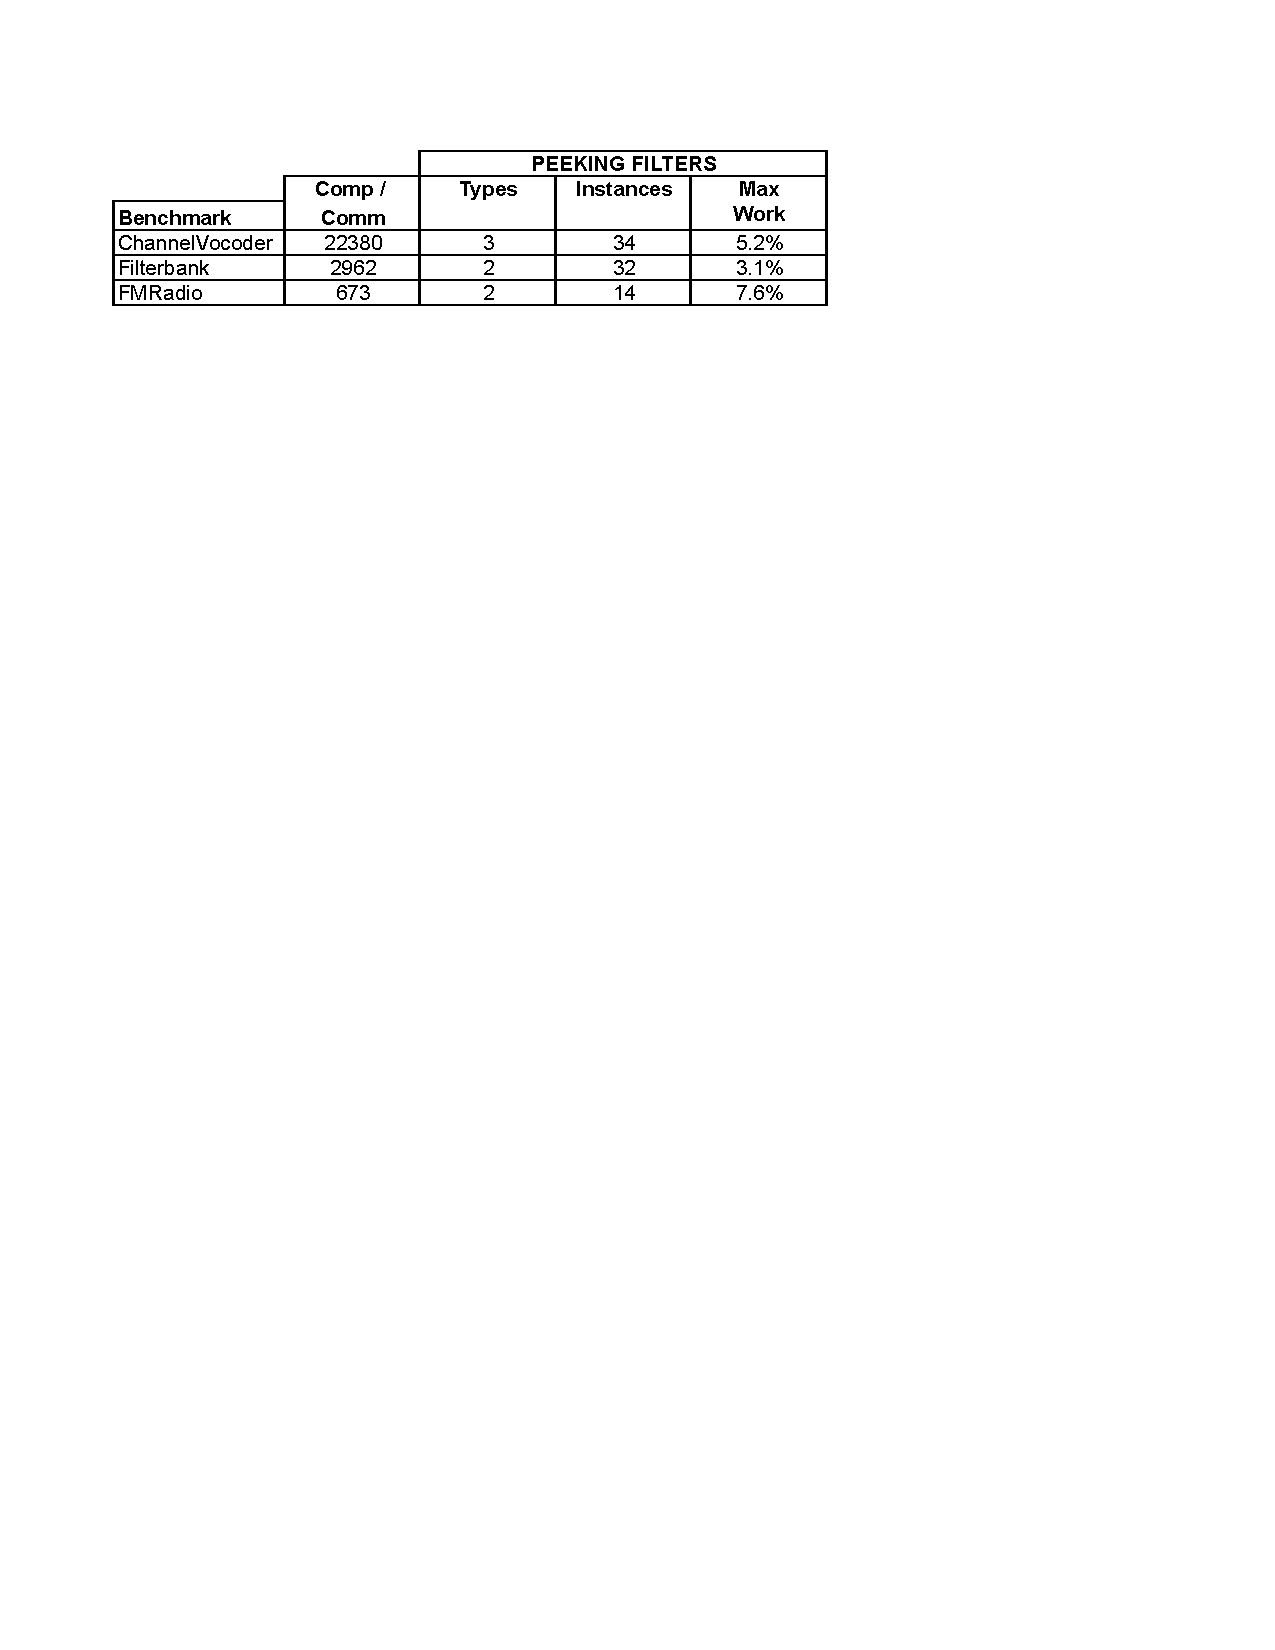
\includegraphics[width=3.3in]{figures/bench-char.pdf}}

\noindent ``Comp/Comm'' provides a static estimation of the
amount of computation to communication ratio by statically estimating the total
work of all the filters and dividing by the number items communicated
for the programmer-conceived graph's steady-state.  The remaining
statistics give the number of peeking filters types, number of peeking
filters instantiated at runtime, and a static estimation of the maximum
work in the single most loaded peeking filter.

We target 2 multicore architecture with different communication
mechanisms.  The Tilera Corporation's TILE64 Processor is a 64 core
system on a chip~\cite{tilera}.  Each core is an identical three-wide
VLIW. The code generated by the StreamIt
compiler for the TILE64 processor follows the remote store programming
(RSP) model~\cite{rsp10} in which each process has a private address
space, but each process can award remote processes write access to
their local memory. When a producer process has write access to a
consumer process's memory, the producer communicates directly with the
consumer via store instructions whose destination is an address in the
consumer's shared memory.  Communication is initiated by the producer,
and is fine-grained.  The consumer reads directly from it's local
memory (L2) when accessing input.

Our symmetric multiprocessor target is a 16-core architecture that is
comprised of four Intel Xeon E7350 multicore processors.  Each processor
is a 64-bit, quad-core with two dual-core dies.  Each die contains a 4
MB L2 cache shared across the two cores.  The front-side bus is clocked
at 1066 MHz.  We utilize the cache coherency mechanism of the
architecture for communication between cores. 

Through empirical experimentation on FMRadio, Filterbank, and
ChannelVocoder, we have settled on $T_{\mt{sharing}} =.10$ and
$T_{\mt{apply}} = 0.05$. These constants are the sweet stop for the two
architectures employed in the experimentation, being a good compromise
between buffer size and inter-core communication.

% \begin{figure*}[t]
% \centering
% \subfigure[]{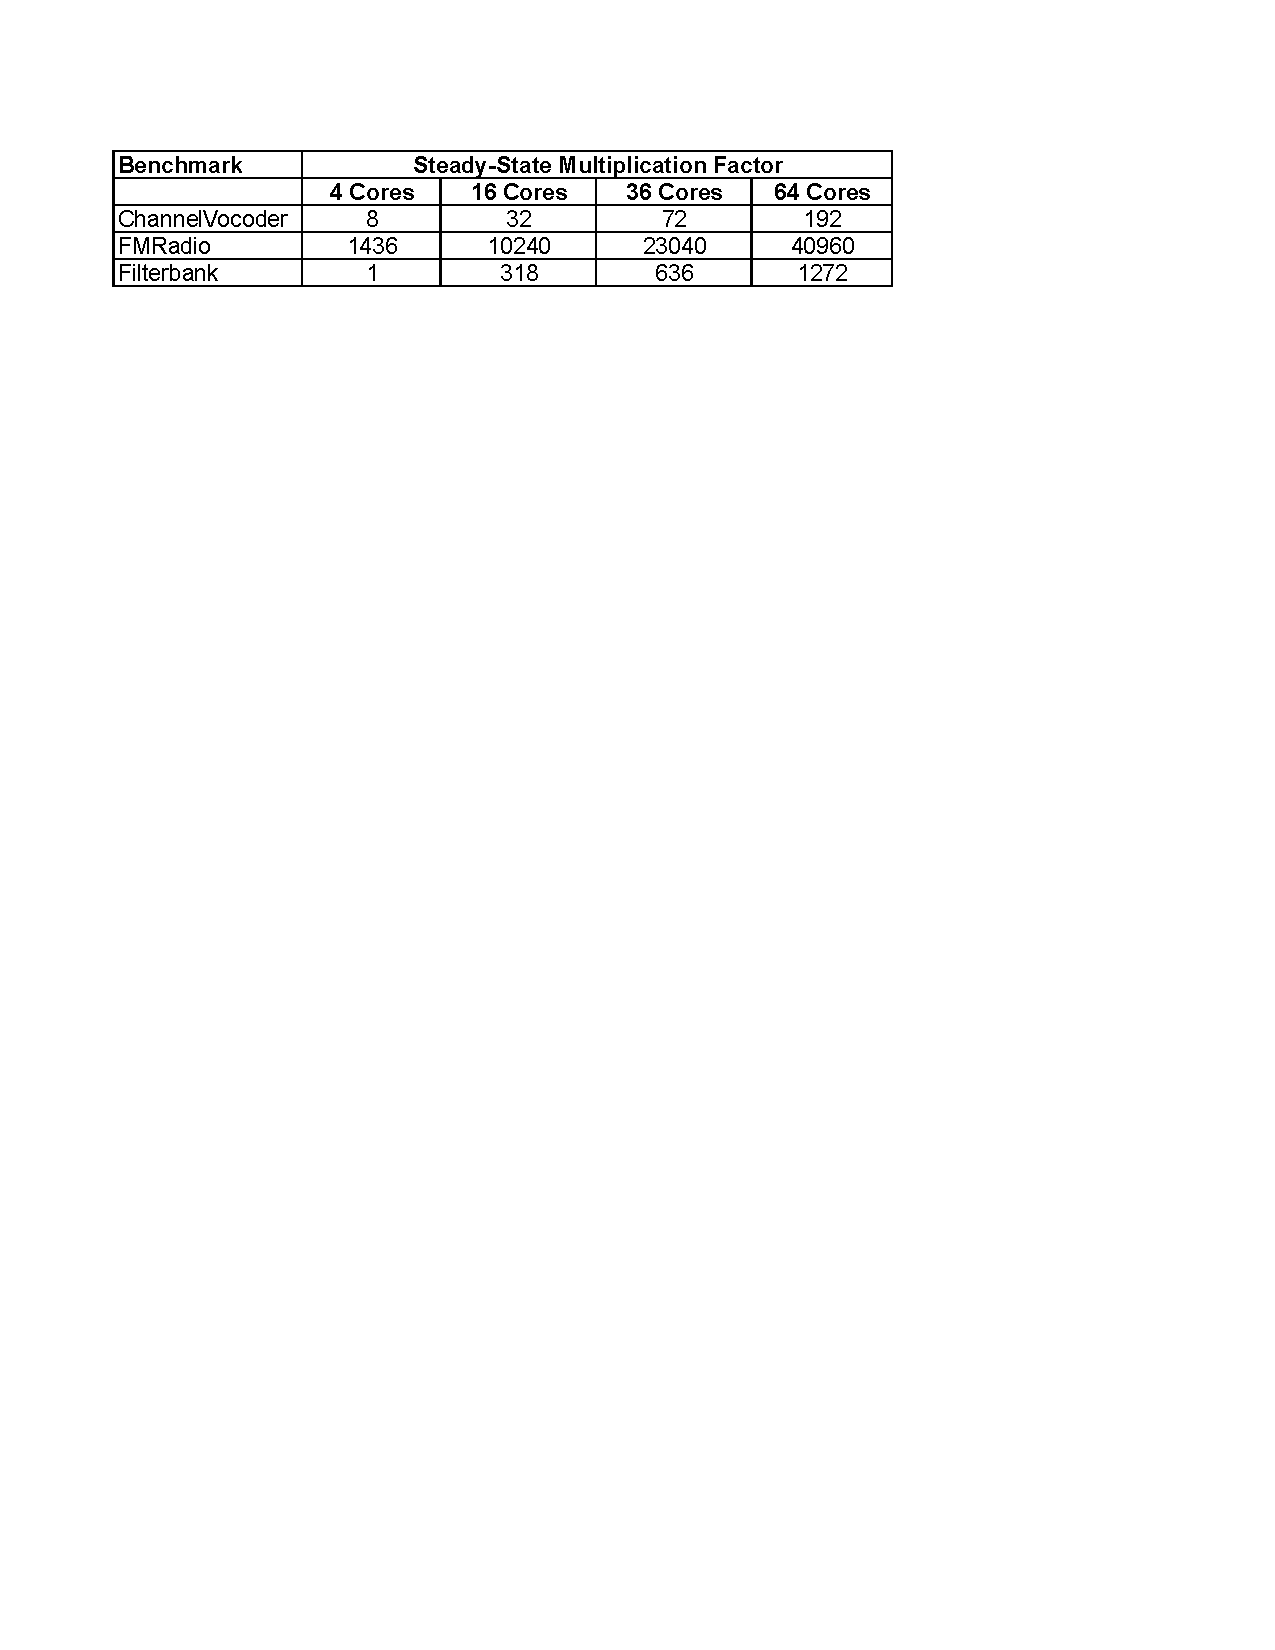
\includegraphics[width=3.7in]{figures/mult-table.pdf}} \\
% \subfigure[]{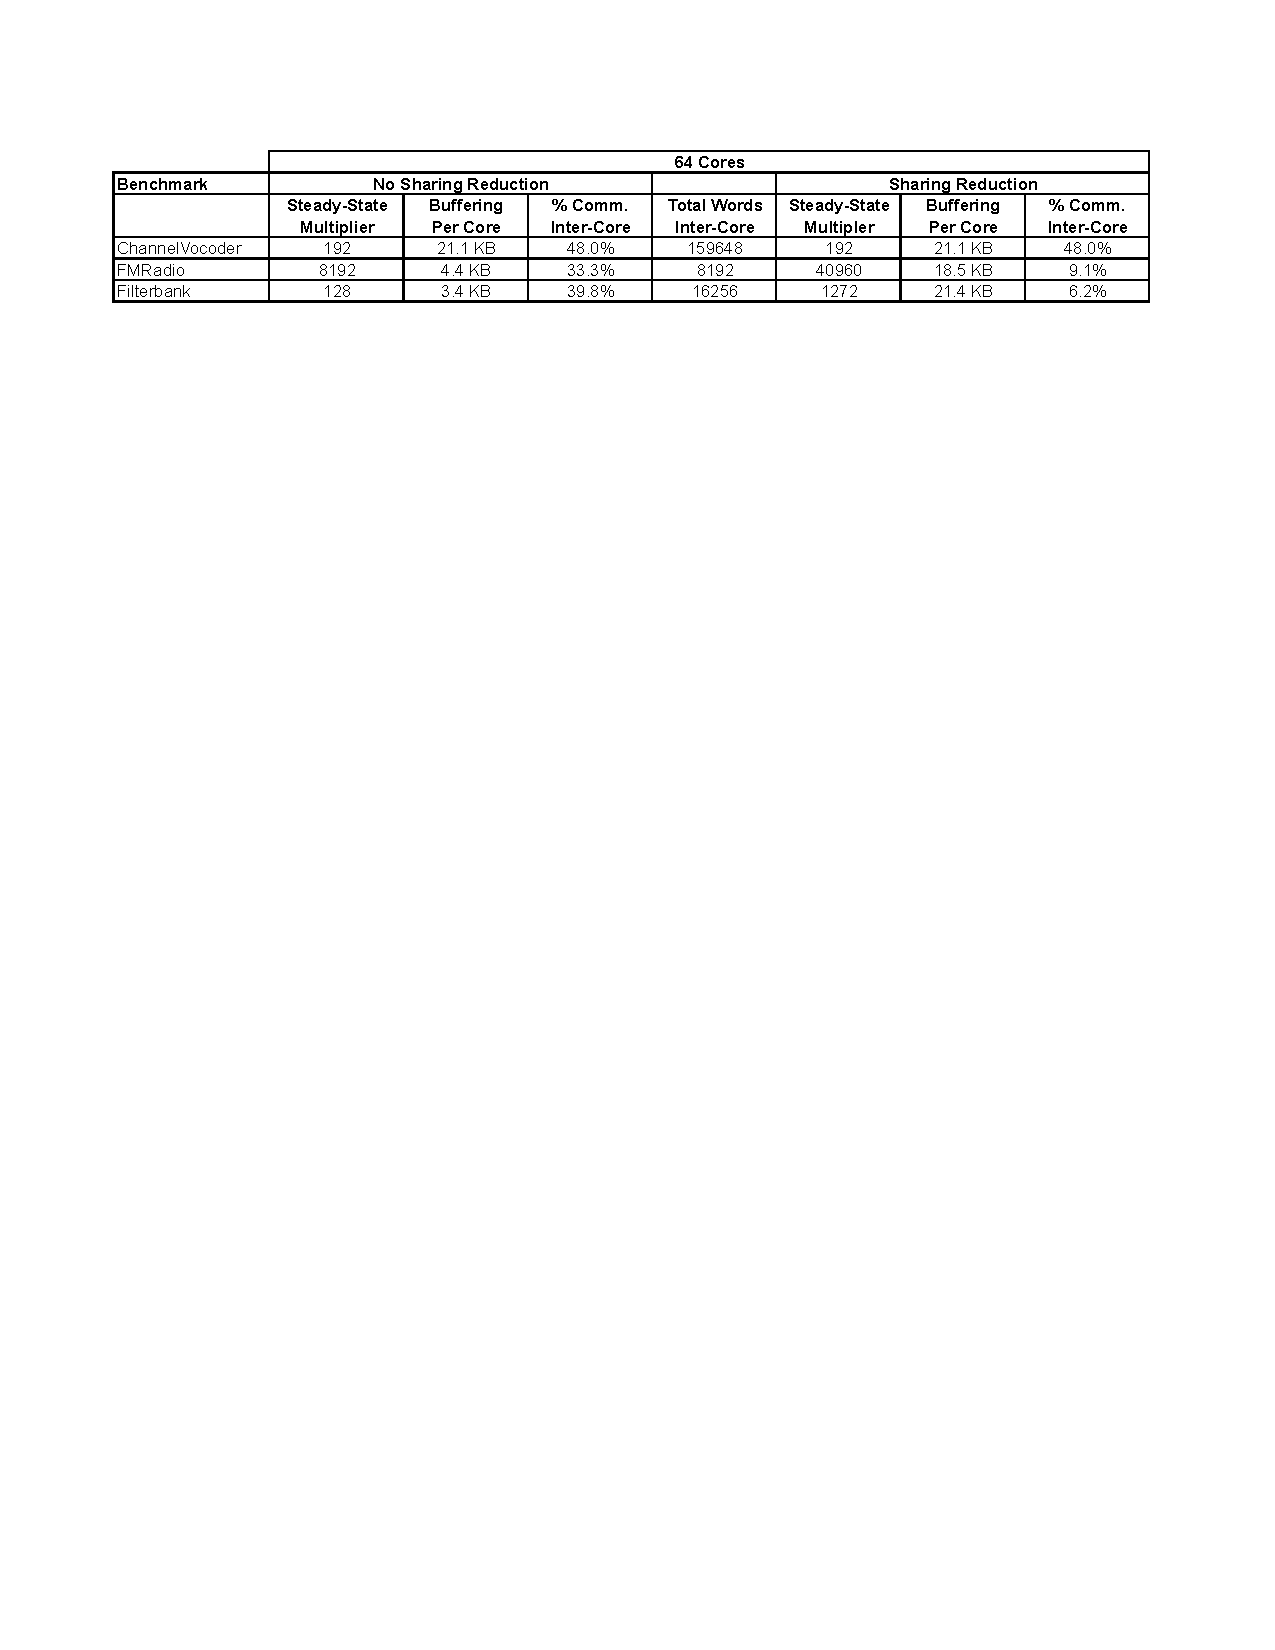
\includegraphics[width=6in]{figures/64-core-table.pdf}}
% \caption[Communication, multiplier and buffering statistics for
% benchmarks.]{
% Communication, multiplier and buffering characteristics for
% benchmarks: (a) gives the steady-state multipliers calculated for
% sharing reduction, (b) compares the steady-state with and without
% sharing reduction. 
% \label{fig:fission-table}}
% \end{figure*}

\begin{figure*}[t]
\centering
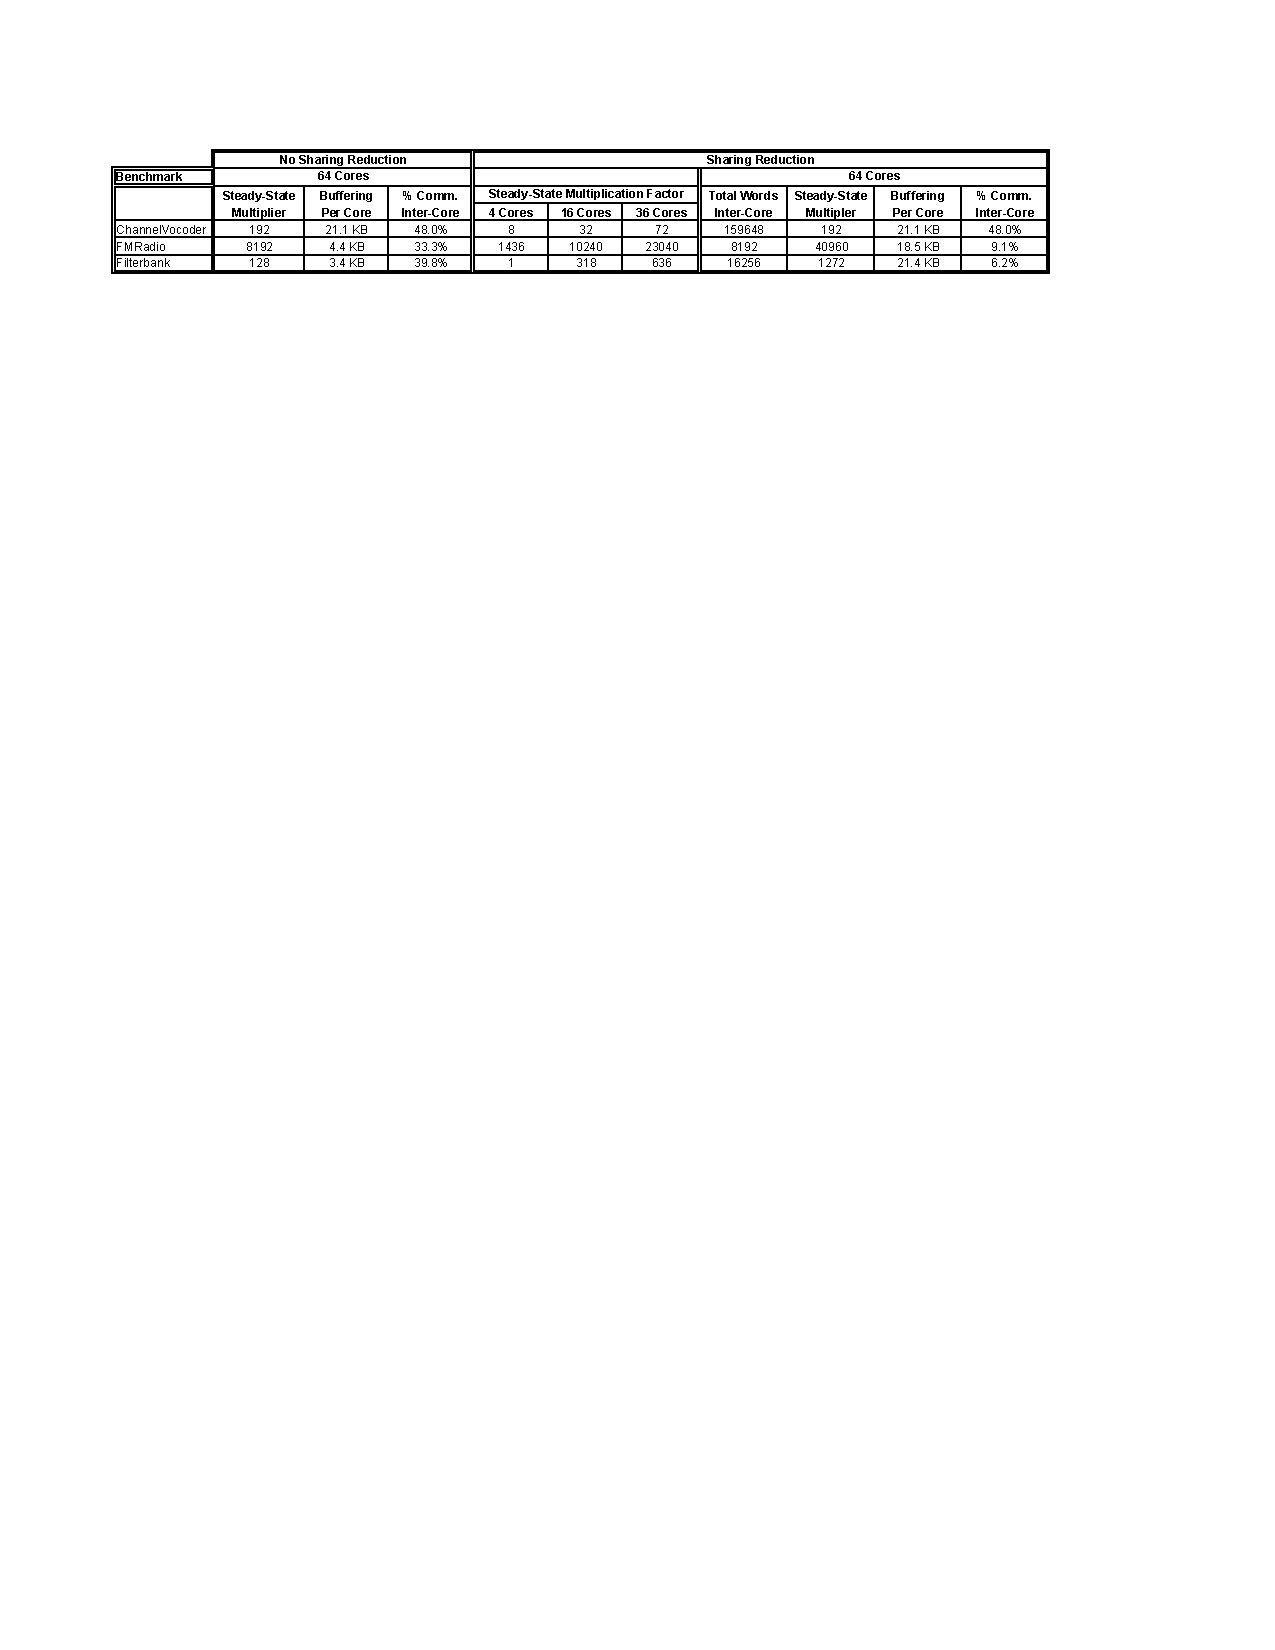
\includegraphics[width=6.1in]{figures/big-table.pdf}
\caption{\label{fig:big-table}  Steady-state multiplicity, buffering,
  and communication for fission with and without sharing reduction.}
\end{figure*}

% \begin{figure}[t]
% \centering
% 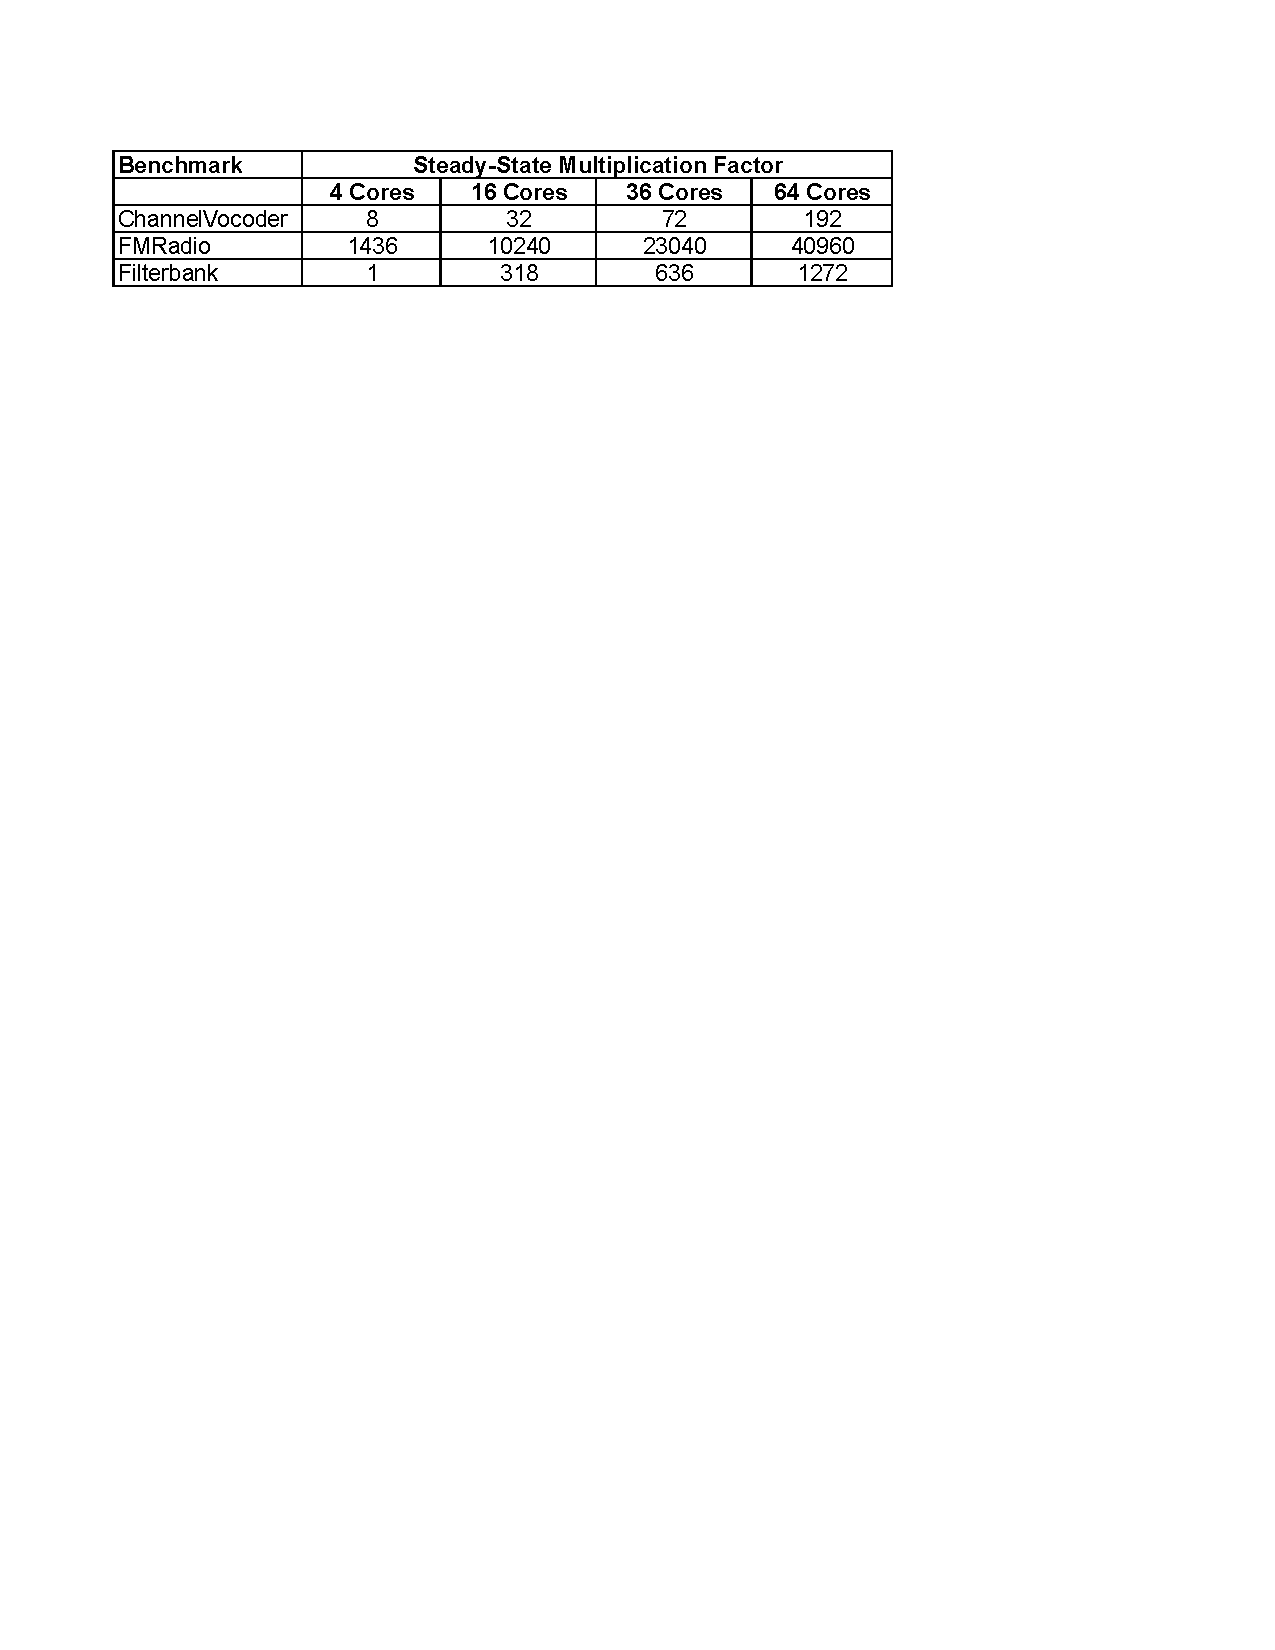
\includegraphics[width=3.3in]{figures/mult-table.pdf}
% \caption{\label{fig:mult-table}  The steady-state multipliers calculated for
% sharing reduction.}
% \end{figure}

% \begin{figure*}[t]
% \centering
% 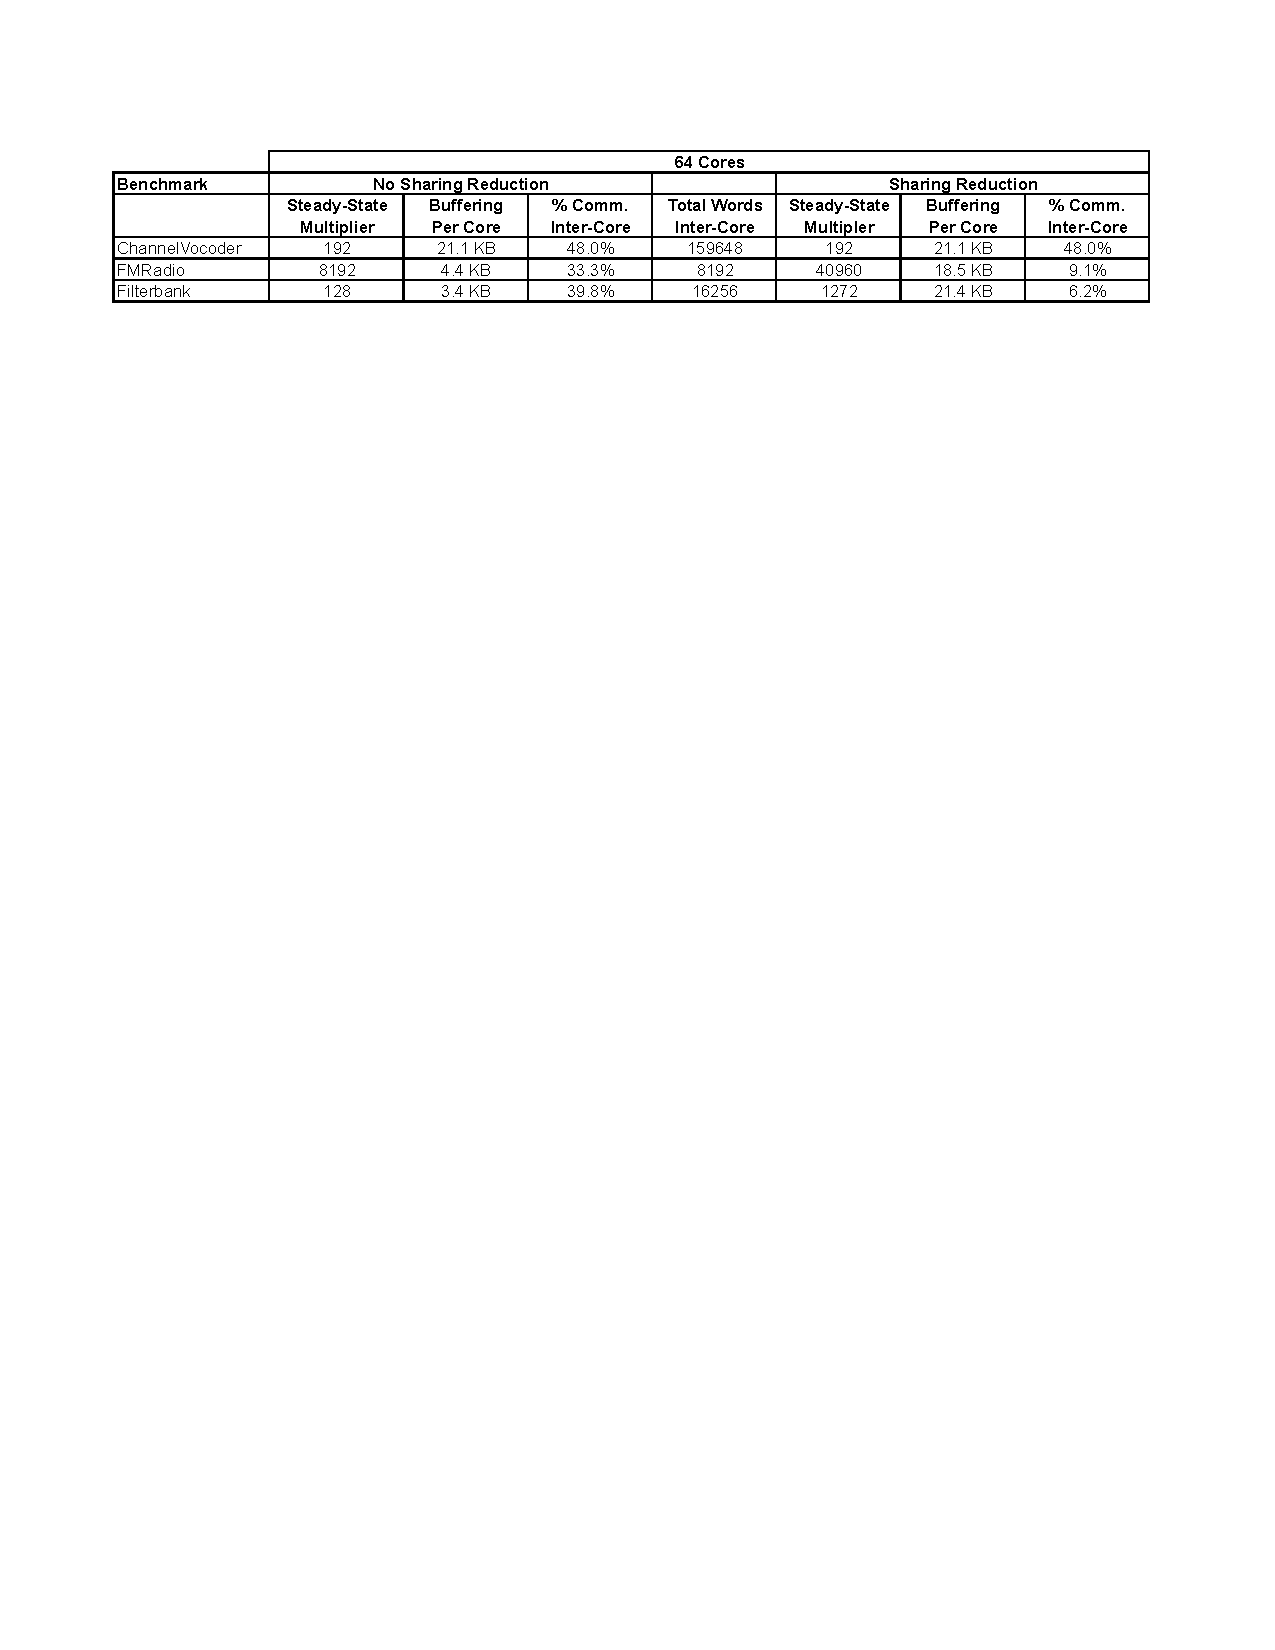
\includegraphics[width=6in]{figures/64-core-table.pdf}
% \caption{ Multiplier, buffering and communication for the steady-state with and without
% sharing reduction. 
% \label{fig:fission-table}}
% \end{figure*}

Figure~\ref{fig:big-table} compares the steady-state with and
without sharing reduction for a 64-core mapping, as well as gives the
constant $c$ calculated by sharing reduction for 4, 16, and 36.  The
factor is larger for FMRadio because one filter has $C(f) \gg o(S,
f)$.  The multiplication factor affects both latency and buffer sizes
adversely.  The application designer will have to decide if the
latency of these techniques can be borne given the application
criteria.  The total buffering requirement is increased when the
steady-state is increased.  However, since we are then fissing, the
buffer is divided amongst the fission products, and the {\it per-core}
buffering requirement is unaffected by the increase.  For example,
FMRadio, has a per-core 18 KB buffering requirement across all
configurations (4, 16, 36, and 64 cores).  This requirement fits in
the per-core L2 size of 64 KB for the Tile64.

 For ChannelVocoder,
sharing reduction has no effect because most of the peeking filters do
not satisfy $T_{\mt{apply}} = 0.05$ because of differing fission
factors between producers and consumers.  For the peeking filters that do,
the steady-state multiplier required for legal general fission for the
graph is enough to assure $T_{\mt{sharing}}$ is met.  Even though
sharing reduction has no effect for ChannelVocoder, general fission
avoids the 38\% of total items that were unnecessary duplicated by
DupDec.

For FMRadio and Filterbank, sharing reduction leads to significant
decreases in the percentage of total items communicated inter-core for
each steady-state.  The buffer requirement is increased an average of
5.2x for these benchmarks.  The total number of words communicated
inter-core during each steady-state is the same, with and without
sharing reduction.  However, the steady-state is greater in the
sharing reduction case, thus producing more outputs.

\begin{figure}[t]
\centering
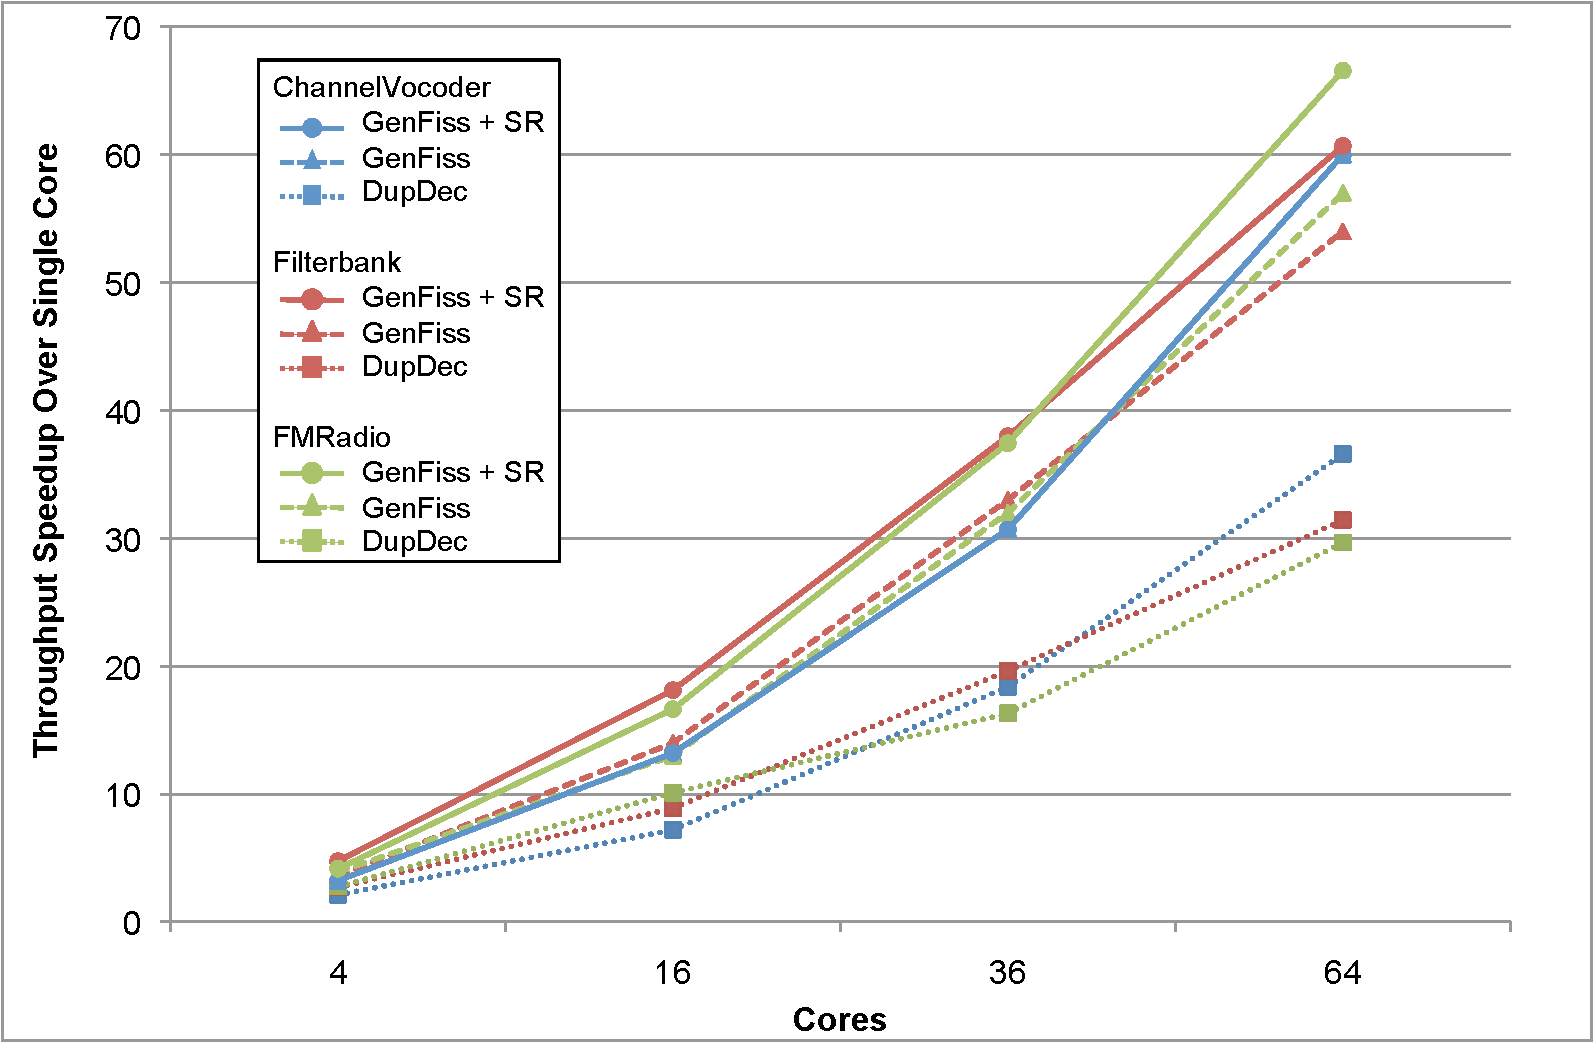
\includegraphics[width=3.3in]{figures/tilera-chart.pdf}
\caption[Comparing the fission techniques on the TILE64.]{
  Evaluation for DupDec versus general fission versus general fission with sharing reduction
  4, 16, 36, and 64 cores on the TILE64.  \label{fig:tilera-chart}}
\end{figure}

Figure~\ref{fig:tilera-chart} gives the performance results for the
Tilera TILE64 architecture.  We present results for DupDec, general
fission, and general fission with sharing reduction for 4, 16, 36, and
64 core configurations, with throughput normalized to single-core
throughput.  General fission with sharing reduction outperforms
DupDec by an average of 1.8x for the three benchmarks when targeting
64 cores. The average 64-core speedup over single core is 62.3x for the
general fission plus sharing reduction for these three benchmarks.

FMRadio experiences the most significant gain from general fission
plus sharing reduction over DupDec (67x versus 30x, respectively, for
64 cores).  FMRadio has the lowest computation to communication ratio
of the 3 benchmarks.  Furthermore, each filter of is fissed by the
number of cores targeted.  For 64 cores, each filter is fissed 64
ways.  DupDec must perform a global all-to-all communication involving
all 64 cores between each level of the graph!
 
ChannelVocoder achieves a 60x speedup for general fission over a
single core.  This is not perfectly linear because of the parallel
mapping; asymmetries exist between the extent of task parallelism and
the number of cores (see~\ref{mgordon-asplos06}).  The speedup over
DupDec (1.62x) is more modest because the width of many of the
fission applications is 3, so DupDec is duplicating input data to
groups of 3 filters.  Filterbank is similar, the width of fission is 4
for all filters when targeting 64 cores.

Sharing reduction is required to achieve scalable speedups for both
FMRadio and Filterbank.  For FMRadio, sharing reductions leads to a
17\% speedup increase for 64 cores.  This because sharing reduction
significantly reduces the number of remote write store instructions
required per output.  This affects FMRadio because of its low
computation to communication ratio.  Sharing reduction sees a 12\%
increase on Filterbank, as Filterbank has a larger computation to
communication ratio.

\begin{figure}[t]
\centering
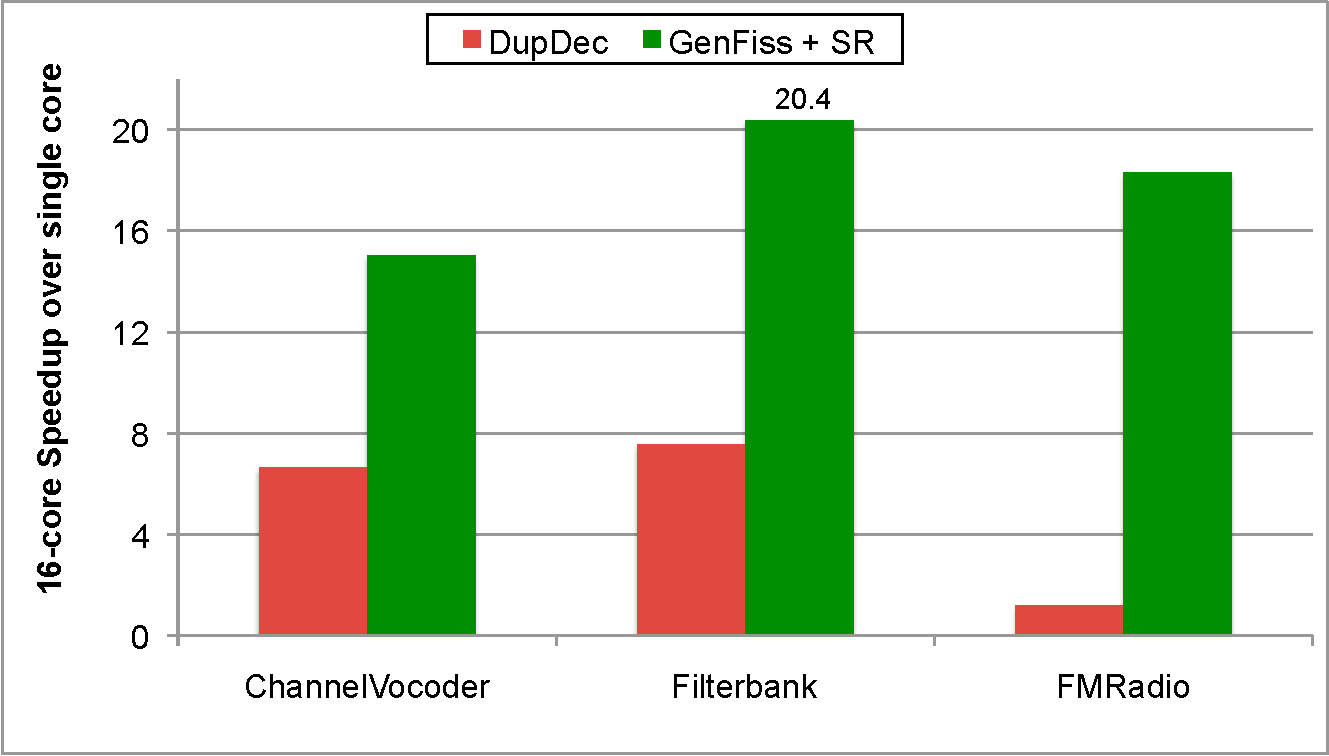
\includegraphics[width=3.3in]{figures/smp-chart.pdf}
\caption[Comparing the fission techniques on the 16-core SMP.]{
  Evaluation for DupDec versus general fission with sharing reduction
  for the 16-core SMP architecture.  \label{fig:smp-chart}}
\end{figure}

Our techniques enable scalable parallelization, with a mean speedup of
17x for our 3 benchmarks on the SMP.  Figure~\ref{fig:smp-chart} gives
the 16-core speedup comparison for DupDec versus general fission with
sharing reduction for our target SMP architecture.  The mean speedup
increase for general fission with sharing reduction over DupDec is
6.7x.  FMRadio again sees the largest speedup increase in the
comparison at 13.0x.  The reasons for this large speedup are similar
as given in the previous section.  However, the SMP communication
mechanism is not as efficient as the TILE64, thus general fission with
sharing reduction gives a greater speedup because reducing inter-core
communication has more impact.

\section{Related Work}
\label{sec:related}

% BILL

%Signal~\cite{Signal}, 
%Lucid~\cite{Lucid77}, and
%Occam~\cite{Occam}, and Sisal \cite{sisal}.
%Parallel Haskell~\cite{ph}
In addition to StreamIt, there are a number of stream-oriented
languages drawing from domains such as functional, dataflow, CSP and
synchronous programming~\cite{survey97}.  The Brook language is
architecture-independent and focusses on data
parallelism~\cite{brook04}.  Stream kernels are required to be
stateless, though there is special support for reducing streams to a
single value.  Stream\-C/Ker\-nel\-C is lower level than Brook;
kernels written in KernelC are stiched together in StreamC and mapped
to the data-parallel Imagine processor~\cite{imagine03ieee}.  SPUR
adopts a similar decomposition between ``microcode'' stream kernels
and skeleton programs to expose data parallelism~\cite{spur05samos}.
Cg exploits pipeline parallelism and data parallelism, though the
programmer must write algorithms to exactly match the two pipeline
stages of a graphics processor~\cite{cg03}.  Compared to these
languages, StreamIt places more emphasis on exposing task and pipeline
parallelism (all the languages expose data parallelim).
%and on sliding window operations (filters that peek).  
By adopting the synchronous dataflow model of execution~\cite{lee87},
StreamIt focusses on well-structured programs that can be aggressively
optimized.  The implicit infinite loop around programs is also a key
StreamIt characteristic that enables the transformations in this
paper.  Spidle is also a recent stream language that was influenced by
StreamIt~\cite{spidle03}.
%and Lucid Synchrone~\cite{Lucid-Synchrone}.
%Synchronous languages which
%target embedded applications include Esterel~\cite{Esterel},
%Lustre~\cite{Lustre}, and Additional

Liao et al. map Brook to multicore processors by leveraging the affine
partitioning model~\cite{liao06brook}.  While affine partitioning is a
powerful model for parameterized loop-based programs, in StreamIt we
simplify the problem by fully resolving the program structure at
compile time.  This allows us to schedule a single steady state using
flexible, non-affine techniques (e.g., simulated annealing) and to
repeat the found schedule for an indefinite period at runtime.
Gummaraju and Rosenblum map stream programs to a general-purpose
hyperthreaded processor~\cite{gummaraju05micro}.  Such techniques
could be integrated with our spatial partitioning to optimize per-core
performance.  Gu et al. expose data and pipeline parallelism in a
Java-like language and use a compiler analysis to efficiently extract
coarse-grained filter boundaries~\cite{du03sc}.  Ottoni et al. also
extract decoupled threads from sequential code, using hardware-based
software pipelining to distribute the resulting threads across
cores~\cite{ottoni05decoupled}.  By embedding pipeline-parallel
filters in the programming model, we focus on the mapping step.

%%%%%%%%%%%%%%%%%%%%%%%%%%%%%%%%%%%%%%%%%%%%%%%%%%%%%%%%%%%%%%%%%%%%%

Previous work in scheduling computation graphs to parallel targets has
focused on partitioning and scheduling techniques that exploit task
and pipeline parallelism~\cite{SDFSched, SDFSched2,may87communicating,
DAGSched, pipeline-sdf}.  Application of loop-conscious
transformations to coarse-grained dataflow graphs has been
investigated.  Unrolling (or ``unfolding'' in this domain) is employed
for synchronous dataflow (SDF) graphs to reduce the initiation
interval but they do not evaluate mappings to actual
architectures~\cite{unfolding,unfolding2}. Software pipelining
techniques have been applied to SDF graphs onto various embedded and
DSP targets~\cite{bakshi99,chatha-02}, but has required programmer
knowledge of both the application and the architecture. To our
knowledge, none of these systems automatically exploit the combination
of task, data, and pipeline parallelism.  Furthermore, these systems
do not provide a robust end-to-end path for application
parallelization from a high-level, portable programming language.

%% Previous work on instruction-level software pipelining has focused
%% mostly on scheduling machine instructions in a loop via modulo
%% scheduling~\cite{rau81,lam-softpipe}.  The algorithms devised must
%% account for tight resource constraints and complex instruction
%% dependences. Our software-pipelining problem is much less constrained,
%% enabling us to employ a simple greedy heuristic.  

%% Furthermore, a traditional modulo scheduling algorithm is not needed
%% because we have an implicit loop barrier at the end of each
%% steady-state.  ILP compilers for clustered VLIW
%% architectures~\cite{Bulldog,Multiflow,lee98spacetime,qian02} must
%% partition instructions and assign them to clusters as part of the
%% instruction scheduling. Clustering is analogous to our application of
%% filter fusion in our software pipelining algorithm.

\section{Conclusion}
\label{sec:conclusion}

In this paper, we describe the StreamIt compiler for the Raw
architecture.  The stream graph of a StreamIt program exposes the data
communication pattern to the compiler while the lack of global
synchronization frees the compiler to radically reoganize the program
for efficient execution on the underline architecture. The StreamIt
compiler demonstrates the power of this flexibility by totally
reoganizing large programs for better load balance. We were able to
map many of programs on to the Raw processor and obtain good
performance.

We introduce a collection of optimizations, vertical and horizontal
filter fusion, vertical and horizontal filter fission and filter
reordering transformations, that can be used to restructure stream
graphs.  We show that by applying these transformations we can map a
high-level stream program, written to reflect the composition of the
application, onto Raw and achieve good processor utilization and load
balance, leading to a factor of three speedup on two applications.

Unlike all previous streaming languages, the structured streams of
StreamIt makes it possible for us to approach the optimization and
parallelization problems in a very systermatic manner. It enables us
to define multiple optimizations -- targetting different constructs
and requirements -- and to compose them them in a hirearchical manner.

The ability to do global transformations across multiple filters, that
may have originated from very different parts of the application,
makes it possible for the compiler to find optimization opportunities
that may ellude even an experience programmer.  Such capabilities
enables the programmers to write protable streaming applications and
map them efficiently onto any given architecture. This has the
potential of creating a programming standard for emerging
communication exposed architectures.  The StreamIt compiler takes a
fist step towards this goal.


%\begin{comment}

\begin{figure}
\begin{center}

\begin{minipage}{1.2in}
\centering \psfig{figure=pipeline-steady-state.eps,width=0.6in} \\
{\protect\small (a) A sample {\pipeline}}
\end{minipage}
~
\begin{minipage}{1.2in}
\centering \psfig{figure=splitjoin-steady-state.eps,width=1.2in} \\
{\protect\small (b) A sample {\splitjoin}}
\end{minipage}
~
\begin{minipage}{1.5in}
\centering \psfig{figure=feedback-steady-state.eps,width=1.0in} \\
{\protect\small (c) A sample {\feedbackloop}.  The $L$ {\filter}
has been flipped upside-down for clarity.\\$peek_L = pop_L = 5,
push_L = 6$}
\end{minipage}

\caption{Sample {\StreamIt} streams} \label{fig:steady-state}

\end{center}
\end{figure}

\subsubsection{\filter}

Since {\filters} do not have any internal buffering, their minimal
steady state is to execute the {\filter}'s {\work} function once.
This is the smallest amount of execution a {\filter} can have.

Thus, for a {\filter} $f$,

\begin{displaymath}
S_f = \left\{[1], \{f\}, { \left[
\begin{array}{c}e_f\\o_f\\u_f
\end{array}
\right]}, [] \right\}
\end{displaymath}

Notice that $S_{f,v}$ is empty, because a {\filter} does not have
any children.

\subsubsection{\pipeline, \splitjoin and \feedbackloop}
\begin{figure}\begin{center}
\begin{minipage}{2in}
\centering \psfig{figure=splitjoin-illegal.eps,width=2in}
\end{minipage}
\end{center}
\caption{An illegal {\splitjoin}} \label{fig:splitjoin-illegal}
\end{figure}


The computation of a steady state for a \pipeline, \splitjoin or a
\feedbackloop is divided into three steps. In the first step we
compute a fractional steady state (a steady state which includes
fractional executions of internal \streams). In the second step we
compute an integral steady state from the fractional steady state.
Finally, we compute a minimal steady state from the integral
steady state.

In order to calculate a fractional steady state of a \stream, we
assign a value of 1 execution for an internal \stream, and iterate
over all the children of the \stream to calculate how many times
they need to execute to consume or produce enough data to conserve
amount of data buffered in the \stream. Here we'll present
specific equations for a \pipeline.

Let the {\pipeline} $p$ have $n$ children and let $p_i$ denote the
$i$th child of the {\pipeline} (counting from {\Input} to
{\Output}, starting with 0, the children may be streams, not
necessarily {\filters}). We must find $S_p$.

We start with calculating all $S_{p_i}, i \in \{0, \dots, n-1\}$.
This task is achieved recursively.

Next we find a fractional vector $v''$ such that executing each
$p_i$ $v_i''$ times will not change the amount of data buffered in
the {\pipeline} and the first child is executed exactly once.
%\begin{comment}
Since the children streams are executed fractional amount of
times, we calculate the amount of data they produce and consume
during this execution by multiplying $S_{p_i,c_o}$ and
$S_{p_i,c_u}$ by $v_i''$.
%\end{comment}
$v''$ must satisfy $v_0'' = 1, \forall i \in \{0,\dots,n-1\},
v_i'' * u_{p_i} = v_{i+1}'' * o_{p_{i-1}}$. Thus
%\begin{comment}
We compute $v''$ as follows.  The first child executes once, thus
$v_0'' = 1$.  The second child must execute $v_1'' = {u_{p_0}
\over {o_{p_1}}}$ times to ensure that all data pushed on the the
first {{\Channel}} is consumed by the second child.  The third
child must execute $v_2'' = v_1'' {u_{p_1} \over o_{p_2}} =
{u_{p_0} \over o_{p_1}} {u_{p_1} \over o_{p_2}}$ times to ensure
that it consumes all the data produced by the second child. Thus,
%\end{comment}
$v_i'' = {\prod_{j = 0}^{i-1} u_{p_j} \over \prod_{j=1}^i
o_{p_j}}$

Next we will find an integral vector $v'$ such that executing each
$p_i$ $v_i'$ times will not change the amount of data buffered in
the {\pipeline}.  $v'$ will be a valid steady state of the
{\pipeline}. In order to calculate $v'$ we multiply $v''$ by
$\prod_{j=1}^{n-1} o_{p_j}$.  Thus

\begin{displaymath}
v'_i = \left({\prod_{j = 0}^{i-1} u_{p_j} \over \prod_{j=1}^i
o_{p_j}} \right) \left(\prod_{j=1}^{n-1} o_{p_j} \right) = \left(
\prod_{j=0}^{i-1} u_{p_j} \right) \left( \prod_{j=i+1}^{n-1}
o_{p_j} \right)
\end{displaymath}

Now we find an integral vector $v$, such that, for some positive
integer $g$, $v' = g * v$, and $\sum_i v_i$ is minimal.  In other
words, we find the greatest integer $g$, such that $v' = g * v$,
with $v$ consisting of integers.  $v$ represents the minimal
steady state for pipeline $p$. This is achieved by finding the
$\gcd$ of all elements in $v'$, and dividing $v'$ by $g$.  Thus $v
= {v' \over \gcd(v')}$

$v$ represents the number of times each child of $p$ will need to
execute its steady state in order to execute the minimal steady
state of $p$, thus $S_{p,v} = v$.  $v$ holds a steady state
because amount of data buffered in $p$ does not change, and it is
a minimal steady state, because $\sum_i v_i$ is minimal.

We construct set $S_p$ as follows:\footnote{Here we use symbol
$\circ$ to denote concatenation of vectors and sets.  Thus $[1\ 2\
3] \circ [4\ 5\ 6] = [1\ 2\ 3\ 4\ 5\ 6]$ and $\{A\ B\ C\} \circ
\{D\ E\ F\} = \{A\ B\ C\ D\ E\ F\}$.}

\begin{displaymath}
S_p = \left\{ \begin{array}{c} v_0 * S_{p_0,m} \circ \dots \circ
v_{n-1}
* S_{p_{n-1}, m}, S_{p_0, N} \circ \dots \circ S_{P_{n-1}, N}, \\
\left[
\begin{array}{c}
e_{p_0} + (v_0 - 1) * o_{p_0} \\
v_0 * o_{p_0} \\
v_{n-1} * u_{p_{n-1}}
\end{array}\right], v \end{array} \right\}
\end{displaymath}

An example is presented in Figure \ref{fig:steady-state} (a). $A$,
$B$, $C$ and $D$ are \filters.
%\begin{comment}For this {\pipeline},
we have the following steady states for all children of the
{\pipeline}:

\begin{displaymath}
\begin{array}{lrlr}
S_A = & \left\{[1], \{A\}, { \left[
\begin{array}{c} 1 \\ 1 \\ 3
\end{array}
\right]}, [] \right\}, &

S_B = & \left\{[1], \{B\}, { \left[
\begin{array}{c} 3 \\ 2 \\ 3
\end{array}
\right]}, [] \right\} \\ \\

S_C = & \left\{[1], \{D\}, { \left[
\begin{array}{c} 2 \\ 2 \\ 1
\end{array}
\right]}, [] \right\}, &

S_D = & \left\{[1], \{D\}, { \left[
\begin{array}{c} 5 \\ 3 \\ 1
\end{array}
\right]}, [] \right\} \\

\end{array}
\end{displaymath}

Using the steady states above, we get the following vector $v'$:

\begin{displaymath}
v' = \left[
\begin{array}{c}
(2 * 2 * 3)\\
(3) (2 * 3) \\
(3 * 3) (3) \\
(3 * 3 * 1)
\end{array}
\right] = \left[
\begin{array}{c}
12\\ 18\\ 27\\ 9
\end{array}
\right]
\end{displaymath}

We now calculate $g = \gcd(v') = \gcd(12,18,27,9) = 3$.  We thus
have

\begin{displaymath}
v = {v' \over 3} = {1 \over 3} \left[
\begin{array}{c}
12\\ 18\\ 27\\ 9
\end{array}
\right] = \left[
\begin{array}{c}
4\\ 6\\ 9\\ 3
\end{array}
\right]
\end{displaymath}

Finally, we construct $S_p$:
%\end{comment}
This \pipeline has the following steady state:

\begin{displaymath}
S_p = \left\{
\begin{array}{c}
4 S_{A,m} \circ 6 S_{B,m} \circ 9 S_{C,m} \circ 3
S_{D,m}, S_{A,N} \circ S_{B,N} \circ S_{C,N} \circ S_{D,N} \\
\left[
\begin{array}{c}
1 + (4-1) * 1 \\
4 * 1 \\
3 * 1
\end{array}\right],
\left[ \begin{array}{c} 4\\ 6\\ 9\\ 3 \end{array} \right]
\end{array}
\right\}
\end{displaymath}

The steady state for \splitjoins and \feedbackloops is computed in
a very similar way. It is important to note that not all
\splitjoins and \feedbackloops have a steady state. It is possible
that one branch of a \splitjoin will produce data at a rate
disproportional to the other branch, thus causing data to
infinitely buffer up inside the \splitjoin. An example of such a
\splitjoin is presented in Figure \ref{fig:splitjoin-illegal}.
Similarly it is possible for a \feedbackloop to consume the data
from the feedback path slower or faster than it is pushed into the
feedback path, thus causing either deadlock or infinite buffering.

%\begin{comment}
\subsubsubsection{\splitjoin}

Let the {\splitjoin} have $n$ children and let $sj_i$ denote the
$i$th child of the {\splitjoin} (counting from left to right,
starting with 0).  Let $sj_s$ and $sj_j$ denote the {\splitter}
and the {\joiner} of the {\splitjoin}, respectively. Let $w_{s,i}$
denote the number of items sent by the {\splitter} to $i$th child
on {\splitter}'s every execution. Let $w_{j,i}$ denote the number
of items consumed by the {\joiner} from the $i$th child on
{\joiner}'s every execution.  We are computing $S_{sj}$.

We start by calculating all $S_{sj_i}, i \in \{0, \dots, n-1\}$.

Next we compute a fraction vector $v''$ and a fraction $a_j''$
such that executing the {\splitter} exactly once, each child
$sj_i$ $v_i''$ times and the {\joiner} $a_j''$ times does not
change the amount of data buffered in the {\splitjoin}. Again,
since $v''$ and $a_j''$ are fractions, we multiply the
steady-state pop and push amounts by appropriate fractions to
obtain the amount of data pushed and popped.  For convenience we
define $a_s''$ to be the number of executions of the {\splitter}
and set it to 1.

%\begin{comment}
\begin{displaymath}
v'', a_j'', a_s'' \ne 0, \forall i \in \{0,\dots,n-1\}, a_s'' *
w_{s, i} = v_i'' * o_{sj_i}, v_i'' * u_{sj_i} = a_j'' * w_{j, i}
\end{displaymath}
\%end{comment}

We thus have that each child $sj_i$ must execute $v_i'' = {w_{s,i}
\over o_{sj_i}}$ times. To compute the number of executions of the
{\joiner}, $a_j''$, we select an arbitrary $k$th child ($0 \le k <
n$) and have that the {\joiner} executes $a_j'' = {{w_{s,k} \over
o_{s_k}}{u_{sj_k} \over w_{j,k}}}$ times.

Next we compute integer vector $v'$ and integers $a_s$ and $a_j$
such that executing the {\splitter} $a_s$ times, each child $sj_i$
$v_i'$ times and the {\joiner} $a_j$ times still does not change
the amount of data buffered in the {\splitjoin}. We do this by
multiplying $a_s''$, $v''$ and $a_j''$ by $w_{j,k}
\left(\prod_{r=0}^{n-1}o_{sj_r}\right)$. Thus we get

\begin{displaymath}
\begin{array}{rl}
a_s' = & w_{j,k} \left(\prod_{r=0}^{n-1}o_{sj_r}\right) \\
v_i' = & w_{j,k} \left(\prod_{r=0}^{n-1}o_{sj_r}\right) * {w_{s,i}
\over o_{sj_i}} = w_{s,i} * w_{j_k} \left( \prod_{r=0}^{i-1}
o_{s_r} \right) \left( \prod_{r=i+1}^{n-1} o_{s_r} \right)
\\
a_j' = & w_{j,k} \left(\prod_{r=0}^{n-1}o_{sj_r}\right) *
{{w_{s,k} \over o_{s_k}}{u_{sj_k} \over w_{j,k}}} = w_{s,k} *
u_{sj_k} * \left( \prod_{r=0}^{k-1} o_{s_r} \right)
\left( \prod_{r=k+1}^{n-1} o_{s_r} \right) \\
\end{array}
\end{displaymath}

Now we use $v'$, $a_s'$ and $a_j'$ to compute minimal steady state
of the {\splitjoin}.  Since $v'$, $a_s'$ and $a_j'$ represent a
steady state, they represent a strict multiple of the minimal
steady state.  Thus we find the multiplier by computing $g$, the
$\gcd$ of all elements in $v'$ and integers $a_s'$ and $a_j'$, and
dividing $v'$, $a_s'$ and $a_j'$ by $g$.  We have that

\begin{displaymath}
\begin{array}{rl}
g = & \gcd(v', a_s', a_j') \\
v = & v' \over g \\
a_s = &  a_s' \over g \\
a_j = & a_j' \over g
\end{array}
\end{displaymath}

Finally, we use $v$, $a_s$ and $a_j$ to construct $S_{sj}$:

\begin{displaymath}
S_{sj} = \left\{
\begin{array}{c}
v_0 * S_{sj_0,m} \circ \dots \circ v_{n-1} * S_{sj_{n-1}, m} \circ
[a_s\ a_j] , \\
S_{sj_0, N} \circ \dots \circ S_{sj_{n-1}, N} \circ \{sj_s,
sj_j\},
\\ \left[
\begin{array}{c}
n_s * o_{s} \\
n_s * o_{s} \\
n_j * u_{j} \\
\end{array}\right], \\
v \circ [a_s] \circ [a_j]
\end{array}\right\}
\end{displaymath}

Figure \ref{fig:steady-state} (b) depicts a sample {\splitjoin}.
The following are the steady states of the {\splitjoin}'s
children: $$
\begin{array}{lrlr} S_A = & \left\{[1], \{A\}, { \left[
\begin{array}{c} 2 \\ 2 \\ 1
\end{array}
\right]}, [] \right\}, & S_B = & \left\{[1], \{B\}, { \left[
\begin{array}{c} 3 \\ 2 \\ 6
\end{array}
\right]}, [] \right\}
\end{array}
$$ For this {\splitjoin}, we select $k = 0$ (we use the left-most child
to compute $a_j'$).  We get the following $v'$, $a_s'$ and $a_j'$

\begin{displaymath}
\begin{array}{rl}
v' = & \left[
\begin{array}{c}
2 * 2 (2)\\
1 * 2 (2)
\end{array}
\right] = \left[
\begin{array}{c}
8 \\ 4
\end{array}
\right] \\
a_s' = & 1 * 2 (2 * 2) = 8 \\
a_j' = & 2 * 1 (2 * 2) = 8
\end{array}
\end{displaymath}

Thus $\gcd(u', a_s', a_j') = \gcd(8,4,8,8) = 4$.  Now we obtain

\begin{displaymath}
\begin{array}{rl}
v = & {v \over 4} = {1 \over 4} \left[
\begin{array}{c}
8 \\ 4
\end{array}
\right] =  \left[
\begin{array}{c}
2 \\ 1
\end{array}
\right]\\
a_s = & {a_s' \over 4} = {8 \over 4} = 2 \\
a_j' = & {a_j' \over 4} = {8 \over 4} = 2
\end{array}
\end{displaymath}

Finally, we construct $S_{sj}$:

\begin{displaymath}
S_{sj} = \left\{
\begin{array}{c}
2 * S_{sj_0, m} \circ 1 * S_{sj_1, m} \circ [2\ 2], \\
S_{sj_0, N} \circ S_{sj_1, N} \circ \{sj_s, sj_j\}, \\
\left[
\begin{array}{c}
2 * 3 \\ 2 * 3 \\ 2 * 4
\end{array}
\right], \left[
\begin{array}{c}
2 \\ 1 \\ 2 \\ 2
\end{array}\right]
\end{array} \right\}
\end{displaymath}

It is important to note, that it is not always possible to compute
a unique $v''$ for all possible {\splitjoins}. The reason is that
unbalanced production/consumption ratios between different
children of a {\splitjoin} can cause data to buffer up infinitely.

\begin{definition}[Valid {\splitjoin}] A {\splitjoin} is valid
{\emph iff} $\forall k, 0 \le k < n-1, a_{j,k}'' = a''_{j,k+1}$,
using notation of $a_{j,k}''$ to indicate that $k$th child of the
{\splitjoin} was used to compute the value of $a_j''$.
\end{definition}

An example of an illegal {\splitjoin} is depicted in Figure
\ref{fig:splitjoin-illegal}.  The rates of throughput of data for
the left child mean that for every execution of the {\splitter},
the {\joiner} needs to be executed exactly once to drain all data
entering the {\splitjoin}.  The rates of throughput of data for
the right child mean that for every execution of the {\splitter},
the {\joiner} needs to be executed exactly twice to drain all data
entering the {\splitjoin}. That means that consumption of data by
the {\joiner} will be relatively slower on the right side, causing
data to buffer up. This means that the given {\splitjoin} does not
have a steady state.

If a {\splitjoin} is such that it does not have a steady state, it
is considered an illegal {\splitjoin}.  It cannot be executed
repeatedly without infinite buffering, so a practical target for
{\StreamIt} cannot execute it.  The calculations presented here
assume that the {\splitjoin} is legal.  In order to check if a
given {\splitjoin} is legal, we test if selecting a different
child for calculation of $a_j''$ yields a different $a_j''$. If it
does, then the two paths tested have different
production/consumption rates, and the {\splitjoin} does not have a
steady state.

\subsubsubsection{\feedbackloop}

Let {\feedbackloop} $fl$ have children $B$ (the body child) and
$L$ (the feedback loop child). Let the {\joiner} and the
{\splitter} of the {\feedbackloop} be denoted $fl_j$ and $fl_s$.
Let $w_{j,I}$ and $w_{j,L}$ denote the number of data items
consumed by the {\joiner} from the {\Input} {{\Channel}} to the
{\feedbackloop} and from $fl_L$, respectively.  Let $w_{s,O}$ and
$w_{s,F}$ denote the number of data items pushed by the
{\splitter} onto the {\feedbackloop}'s {\Input} {{\Channel}} and
to $fl_L$ respectively.  We are computing $S_{fl}$.

First we calculate $S_{B}$ and $S_{L}$.

Now we compute a fractional vector $v'' = [a_B''\ a_L''\ a_s''\
a_j'']$ such that executing the body child $a_B''$ times, the
{\splitter} $a_s''$ times, the loop child $a_F''$ times and the
{\joiner} $a_j''$ times will not change the amount of data
buffered up in the {\feedbackloop}.  Thus

\begin{displaymath}
\begin{array}{rcl}
a_B' * u_B & = & a_s' * o_s \\
a_L' * u_B & = & a_j' * w_{j, L} \\
a_s' * w_{s, F} & = & a_L' * o_B \\
a_j' * u_j & = & a_B' * o_B \\
\end{array}
\end{displaymath}

We begin with setting $a_j'' = 1$. $B$ needs to be executed $a_B''
= u_j \over o_B$ times, the {\splitter} needs to be executed
$a_s'' = {u_j \over o_B}{u_B \over o_s}$ times and $L$ needs to be
executed $a_L'' = {u_j \over o_B}{u_B \over o_s}{w_{s,L} \over
o_L}$ times. Furthermore, in order to assure that the
{\feedbackloop} has a valid steady state, we continue going around
the loop, the {\joiner} must require ${u_j \over o_B}{u_B \over
o_s}{w_{s,L} \over o_L}{u_L \over w_{j,L}} = 1$.  If this
condition is not satisfied, the {\feedbackloop} does not have a
steady state. This is a necessary, but not a sufficient condition
for a {\feedbackloop} to be valid.

Next we compute an integer vector $v' = [a_B'\ a_L'\ a_s'\ a_j']$
such that executing B $a_B'$ times, {\splitter} $a_s'$ times, L
$a_L'$ times and {\joiner} $a_j'$ times will not change the amount
of data buffered in the {\splitjoin}. We do this by multiplying
$v''$ by $o_B * o_s * o_L$.

\begin{displaymath}
\begin{array}{rl}
a_B' = & u_j * o_s * o_L \\
a_L' = & u_j * u_B * w_{s,L} \\
a_j = & o_B * o_s * o_L \\
a_s = & u_j * u_B * o_L
\end{array}
\end{displaymath}

We now use $v'$ to compute $v = [a_B\ a_L\ a_s\ a_j]$, a minimal
steady state for the {\feedbackloop}.  We do this by finding an
integer $g$, the $\gcd$ of all elements in $v'$ and computing $v =
{v' \over g}$.

Finally, we construct $S_{fj}$ as follows:

\begin{displaymath}
S_{fj} = \left\{
\begin{array}{c}
a_B * S_{B,m} \circ a_L * S_{L,m} \circ [a_s \ a_j], \\
S_{B,N} \circ S_{L,N} \circ \{fl_s, fl_j\}, \\
\left[\begin{array}{c}
a_j * w_{j,I} \\
a_j * w_{j,I} \\
a_s * w_{s,O}
\end{array} \right], v
\end{array} \right\}
\end{displaymath}

Figure \ref{fig:steady-state}(c) depicts a sample {\feedbackloop}.
The following are the steady states of the {\splitjoin}'s
children:
$$
\begin{array}{lrlr} S_B = & \left\{[1], \{B\}, { \left[
\begin{array}{c} 2 \\ 2 \\ 1
\end{array}
\right]}, [] \right\}, & S_L = & \left\{[1], \{L\}, { \left[
\begin{array}{c} 5 \\ 5 \\ 6
\end{array}
\right]}, [] \right\}
\end{array}
$$ We compute $v'$ for this {\feedbackloop}:

\begin{displaymath}
v' = \left[
\begin{array}{c}
5 * 3 * 5 \\
5 * 1 * 3 \\
5 * 1 * 5 \\
2 * 3 * 5
\end{array}\right] = \left[
\begin{array}{c}
75 \\
15 \\
25 \\
30
\end{array}\right]
\end{displaymath}

Thus $g = \gcd(75,15,25,30) = 5$ and

\begin{displaymath}
v = {1 \over 5} \left[
\begin{array}{c}
15 \\
3 \\
5 \\
6
\end{array}\right]
\end{displaymath}

Finally, we construct $S_{fl}$

\begin{displaymath}
S_{fl} = \left\{
\begin{array}{c}
15 * S_{B, m} \circ 3 * S_{L, m} \circ [5\ 6], \\
S_{B, N} \circ S_{L, N} \circ \{fl_s, fl_j\}, \\
\left[
\begin{array}{c}
6 * 2 \\ 6 * 2 \\ 5 * 3
\end{array}
\right], \left[
\begin{array}{c}
15 \\ 3 \\ 5 \\ 6
\end{array}\right]
\end{array} \right\}
\end{displaymath}
%\end{comment}

\end{comment}


\appendix
\section{Details of Calculating Minimal Steady States}
\label{apx:eqs}

This appendix presents equations used for calculating minimal
steady states.  Minimal steady states are calculated recursively
in a hierarchical manner. That is, a minimal steady state is
calculated for all children streams of {\pipeline}, {\splitjoin}
and {{\feedbackloop}}, and then the schedule is computed for the
actual parent stream using these minimal states as atomic
executions. This yields a minimal steady state because all child
streams must execute their steady states (to avoid buffering
changes), and all steady states are multiples of the minimal
steady states (per Theorem \ref{thm:multiplicity}).  Executing a
full steady state of a stream is referred to as ``executing a
stream.''

\begin{figure}
\begin{center}

\begin{minipage}{1.5in}
\centering \psfig{figure=pipeline-steady-state.eps,width=0.6in} \\
{\protect\small (a) A sample {\pipeline}}
\end{minipage}
~
\begin{minipage}{1.5in}
\centering \psfig{figure=splitjoin-steady-state.eps,width=1.2in} \\
{\protect\small (b) A sample {\splitjoin}}
\end{minipage}
~
\begin{minipage}{2in}
\centering \psfig{figure=feedback-steady-state.eps,width=1.0in} \\
{\protect\small (c) A sample {{\feedbackloop}}.  The $L$ {\filter}
has been flipped upside-down for clarity.\\$peek_L = pop_L = 5,
push_L = 6$}
\end{minipage}

\caption{Sample {\StreamIt} streams. These are identical to
streams in Figure \ref{fig:steady-state}, except for the
{\pipeline}.} \label{fig:app:steady-state}

\end{center}
\end{figure}

\subsection{\filter}

Since {\filters} do not have any internal buffering, their minimal
steady state is to execute the {\filter}'s {\work} function once.
This is the smallest amount of execution a {\filter} can have.

Thus, for a {\filter} $f$,

\begin{displaymath}
S_f = \left\{[1], \{f\}, { \left[
\begin{array}{c}e_f\\o_f\\u_f
\end{array}
\right]}, [] \right\}
\end{displaymath}

Notice that $S_{f,v}$ is empty, because a {\filter} does not have
any children.

\subsection{\pipeline}

Let the {\pipeline} $p$ have $n$ children and let $p_i$ denote the
$i$th child of the {\pipeline} (counting from {\Input} to
{\Output}, starting with 0, the children may be streams, not
necessarily {\filters}). We must find $S_p$.

We start with calculating all $S_{p_i}, i \in \{0, \dots, n-1\}$.
This task is achieved recursively.

Next we find a fractional vector $v''$ such that executing each
$p_i$ $v_i''$ times will not change the amount of data buffered in
the {\pipeline} and the first child is executed exactly once.
Since the children streams are executed fractional amount of
times, we calculate the amount of data they produce and consume
during this execution by multiplying $S_{p_i,c_o}$ and
$S_{p_i,c_u}$ by $v_i''$. Thus $v''$ must have the following
property

\begin{displaymath}
v_0'' = 1, \forall i \in \{0,\dots,n-2\}, v_i'' * u_{p_i} =
v_{i+1}'' * o_{p_{i+1}}
\end{displaymath}

We compute $v''$ as follows.  The first child executes once, thus
$v_0'' = 1$.  The second child must execute $v_1'' = {u_{p_0}
\over {o_{p_1}}}$ times to ensure that all data pushed on the the
first {{\Channel}} is consumed by the second child.  The third
child must execute $v_2'' = v_1'' {u_{p_1} \over o_{p_2}} =
{u_{p_0} \over o_{p_1}} {u_{p_1} \over o_{p_2}}$ times to ensure
that it consumes all the data produced by the second child. Thus,

\begin{displaymath}
\forall i \in \{1,\dots,n-1\}\ v_i'' = {\prod_{j = 0}^{i-1}
u_{p_j} \over \prod_{j=1}^i o_{p_j}}
\end{displaymath}

Next we will find an integral vector $v'$ such that executing each
$p_i$ $v_i'$ times will not change the amount of data buffered in
the {\pipeline}.  $v'$ will be a valid steady state of the
{\pipeline}.

In order to calculate $v'$ we multiply $v''$ by $\prod_{j=1}^{n-1}
o_{p_j}$.  Thus

\begin{displaymath}
v'_i = \left({\prod_{j = 0}^{i-1} u_{p_j} \over \prod_{j=1}^i
o_{p_j}} \right) \left(\prod_{j=1}^{n-1} o_{p_j} \right) = \left(
\prod_{j=0}^{i-1} u_{p_j} \right) \left( \prod_{j=i+1}^{n-1}
o_{p_j} \right)
\end{displaymath}

Now we find an integral vector $v$, such that, for some positive
integer $g$, $v' = g * v$, and $\sum_i v_i$ is minimal.  In other
words, we find the greatest integer $g$, such that $v' = g * v$,
with $v$ consisting of integers.  $v$ represents the minimal
steady state for pipeline $p$.

This is achieved by finding the $\gcd$ of all elements in $v'$,
and dividing $v'$ by $g$.  Thus

\begin{displaymath}
v = {v' \over \gcd(v'_0,\dots,v'_{n-1})}
\end{displaymath}

$v$ represents the number of times each child of $p$ will need to
execute its steady state in order to execute the minimal steady
state of $p$, thus $S_{p,v} = v$.  $v$ holds a steady state
because amount of data buffered in $p$ does not change, and it is
a minimal steady state, because $\sum_i v_i$ is minimal.

We construct set $S_p$ as follows:\footnote{Here we use symbol
$\circ$ to denote concatenation of vectors and sets.  Thus $[1\ 2\
3] \circ [4\ 5\ 6] = [1\ 2\ 3\ 4\ 5\ 6]$ and $\{A\ B\ C\} \circ
\{D\ E\ F\} = \{A\ B\ C\ D\ E\ F\}$.}

\begin{displaymath}
S_p = \left\{ \begin{array}{c} v_0 * S_{p_0,m} \circ \dots \circ
v_{n-1}
* S_{p_{n-1}, m}, S_{p_0, N} \circ \dots \circ S_{p_{n-1}, N}, \\
\left[
\begin{array}{c}
e_{p_0} + (v_0 - 1) * o_{p_0} \\
v_0 * o_{p_0} \\
v_{n-1} * u_{p_{n-1}}
\end{array}\right], v \end{array} \right\}
\end{displaymath}

An example is presented in Figure \ref{fig:app:steady-state} (a).
For this {\pipeline}, we have the following steady states for all
children of the {\pipeline}:

\begin{displaymath}
\begin{array}{lrlr}
S_A = & \left\{[1], \{A\}, { \left[
\begin{array}{c} 1 \\ 1 \\ 3
\end{array}
\right]}, [] \right\}, &

S_B = & \left\{[1], \{B\}, { \left[
\begin{array}{c} 3 \\ 2 \\ 3
\end{array}
\right]}, [] \right\} \\ \\

S_C = & \left\{[1], \{D\}, { \left[
\begin{array}{c} 2 \\ 2 \\ 1
\end{array}
\right]}, [] \right\}, &

S_D = & \left\{[1], \{D\}, { \left[
\begin{array}{c} 5 \\ 3 \\ 1
\end{array}
\right]}, [] \right\} \\

\end{array}
\end{displaymath}

Using the steady states above, we get the following vector $v'$:

\begin{displaymath}
v' = \left[
\begin{array}{c}
(2 * 2 * 3)\\
(3) (2 * 3) \\
(3 * 3) (3) \\
(3 * 3 * 1)
\end{array}
\right] = \left[
\begin{array}{c}
12\\ 18\\ 27\\ 9
\end{array}
\right]
\end{displaymath}

We now calculate $g = \gcd(v') = \gcd(12,18,27,9) = 3$.  We thus
have

\begin{displaymath}
v = {v' \over 3} = {1 \over 3} \left[
\begin{array}{c}
12\\ 18\\ 27\\ 9
\end{array}
\right] = \left[
\begin{array}{c}
4\\ 6\\ 9\\ 3
\end{array}
\right]
\end{displaymath}

Finally, we construct $S_p$:

\begin{displaymath}
S_p = \left\{
\begin{array}{c}
4 S_{A,m} \circ 6 S_{B,m} \circ 9 S_{C,m} \circ 3
S_{D,m}, S_{A,N} \circ S_{B,N} \circ S_{C,N} \circ S_{D,N} \\
\left[
\begin{array}{c}
1 + (4-1) * 1 \\
4 * 1 \\
3 * 1
\end{array}\right],
\left[ \begin{array}{c} 4\\ 6\\ 9\\ 3 \end{array} \right]
\end{array}
\right\}
\end{displaymath}

\subsection{\splitjoin}

Let the {\splitjoin} have $n$ children and let $sj_i$ denote the
$i$th child of the {\splitjoin} (counting from left to right,
starting with 0).  Let $sj_s$ and $sj_j$ denote the {\splitter}
and the {\joiner} of the {\splitjoin}, respectively. Let $w_{s,i}$
denote the number of items sent by the {\splitter} to $i$th child
on {\splitter}'s every execution. Let $w_{j,i}$ denote the number
of items consumed by the {\joiner} from the $i$th child on
{\joiner}'s every execution.  We are computing $S_{sj}$.

We start by calculating all $S_{sj_i}, i \in \{0, \dots, n-1\}$.

Next we compute a fraction vector $v''$ and a fraction $a_j''$
such that executing the {\splitter} exactly once, each child
$sj_i$ $v_i''$ times and the {\joiner} $a_j''$ times does not
change the amount of data buffered on any {\Channel} in the
{\splitjoin}. Again, since $v''$ and $a_j''$ are fractions, we
multiply the steady-state pop and push amounts by appropriate
fractions to obtain the amount of data pushed and popped.  For
convenience we define $a_s''$ to be the number of executions of
the {\splitter} and set it to 1.

\begin{comment}
\begin{displaymath}
v'', a_j'', a_s'' \ne 0, \forall i \in \{0,\dots,n-1\}, a_s'' *
w_{s, i} = v_i'' * o_{sj_i}, v_i'' * u_{sj_i} = a_j'' * w_{j, i}
\end{displaymath}
\end{comment}

We thus have that each child $sj_i$ must execute $v_i'' = {w_{s,i}
\over o_{sj_i}}$ times. To compute the number of executions of the
{\joiner}, $a_j''$, we select an arbitrary $k$th child ($0 \le k <
n$) and have that the {\joiner} executes $a_j'' = {{w_{s,k} \over
o_{s_k}}{u_{sj_k} \over w_{j,k}}}$ times.

Next we compute integer vector $v'$ and integers $a_s$ and $a_j$
such that executing the {\splitter} $a_s$ times, each child $sj_i$
$v_i'$ times and the {\joiner} $a_j$ times still does not change
the amount of data buffered on any {\Channel} in the {\splitjoin}.
We do this by multiplying $a_s''$, $v''$ and $a_j''$ by $w_{j,k}
\left(\prod_{r=0}^{n-1}o_{sj_r}\right)$. Thus we get

\begin{displaymath}
\begin{array}{rl}
a_s' = & w_{j,k} \left(\prod_{r=0}^{n-1}o_{sj_r}\right) \\
v_i' = & w_{j,k} \left(\prod_{r=0}^{n-1}o_{sj_r}\right) * {w_{s,i}
\over o_{sj_i}} = w_{s,i} * w_{j_k} \left( \prod_{r=0}^{i-1}
o_{s_r} \right) \left( \prod_{r=i+1}^{n-1} o_{s_r} \right)
\\
a_j' = & w_{j,k} \left(\prod_{r=0}^{n-1}o_{sj_r}\right) *
{{w_{s,k} \over o_{s_k}}{u_{sj_k} \over w_{j,k}}} = w_{s,k} *
u_{sj_k} * \left( \prod_{r=0}^{k-1} o_{s_r} \right)
\left( \prod_{r=k+1}^{n-1} o_{s_r} \right) \\
\end{array}
\end{displaymath}

Now we use $v'$, $a_s'$ and $a_j'$ to compute minimal steady state
of the {\splitjoin}.  Since $v'$, $a_s'$ and $a_j'$ represent a
steady state, they represent a strict multiple of the minimal
steady state.  Thus we find the multiplier by computing $g$, the
$\gcd$ of all elements in $v'$ and integers $a_s'$ and $a_j'$, and
dividing $v'$, $a_s'$ and $a_j'$ by $g$.  We have that

\begin{displaymath}
\begin{array}{rl}
g = & \gcd(v', a_s', a_j') \\
v = & v' \over g \\
a_s = &  a_s' \over g \\
a_j = & a_j' \over g
\end{array}
\end{displaymath}

Finally, we use $v$, $a_s$ and $a_j$ to construct $S_{sj}$:

\begin{displaymath}
S_{sj} = \left\{
\begin{array}{c}
v_0 * S_{sj_0,m} \circ \dots \circ v_{n-1} * S_{sj_{n-1}, m} \circ
\left[\begin{array}{c}a_s\\a_j\end{array}\right] , \\
S_{sj_0, N} \circ \dots \circ S_{sj_{n-1}, N} \circ \{sj_s,
sj_j\},
\\ \left[
\begin{array}{c}
n_s * o_{s} \\
n_s * o_{s} \\
n_j * u_{j} \\
\end{array}\right], \\
v \circ [a_s] \circ [a_j]
\end{array}\right\}
\end{displaymath}

Figure \ref{fig:steady-stat}e (b) depicts a sample {\splitjoin}.
The following are the steady states of the {\splitjoin}'s
children: $$
\begin{array}{lrlr} S_A = & \left\{[1], \{A\}, { \left[
\begin{array}{c} 2 \\ 2 \\ 1
\end{array}
\right]}, [] \right\}, & S_B = & \left\{[1], \{B\}, { \left[
\begin{array}{c} 3 \\ 2 \\ 6
\end{array}
\right]}, [] \right\}
\end{array}
$$ For this {\splitjoin}, we select $k = 0$ (we use the left-most child
to compute $a_j'$).  We get the following $v'$, $a_s'$ and $a_j'$

\begin{displaymath}
\begin{array}{rl}
v' = & \left[
\begin{array}{c}
2 * 2 (2)\\
1 * 2 (2)
\end{array}
\right] = \left[
\begin{array}{c}
8 \\ 4
\end{array}
\right] \\
a_s' = & 1 * 2 (2 * 2) = 8 \\
a_j' = & 2 * 1 (2 * 2) = 8
\end{array}
\end{displaymath}

Thus $\gcd(u', a_s', a_j') = \gcd(8,4,8,8) = 4$.  Now we obtain

\begin{displaymath}
\begin{array}{rl}
v = & {v \over 4} = {1 \over 4} \left[
\begin{array}{c}
8 \\ 4
\end{array}
\right] =  \left[
\begin{array}{c}
2 \\ 1
\end{array}
\right]\\
a_s = & {a_s' \over 4} = {8 \over 4} = 2 \\
a_j' = & {a_j' \over 4} = {8 \over 4} = 2
\end{array}
\end{displaymath}

Finally, we construct $S_{sj}$:

\begin{displaymath}
S_{sj} = \left\{
\begin{array}{c}
2 * S_{sj_0, m} \circ 1 * S_{sj_1, m} \circ \left[\begin{array}{c}2\\2\end{array}\right], \\
S_{sj_0, N} \circ S_{sj_1, N} \circ \{sj_s, sj_j\}, \\
\left[
\begin{array}{c}
2 * 3 \\ 2 * 3 \\ 2 * 4
\end{array}
\right], \left[
\begin{array}{c}
2 \\ 1 \\ 2 \\ 2
\end{array}\right]
\end{array} \right\}
\end{displaymath}

\begin{figure}\begin{center}
\begin{minipage}{1in}
\centering \psfig{figure=splitjoin-illegal.eps,width=2in}
\end{minipage}
\end{center}
\caption{An illegal {\splitjoin}} \label{fig:splitjoin-illegal}
\end{figure}

It is important to note, that it is not always possible to compute
a unique $v''$ for all possible {\splitjoins}. The reason is that
unbalanced production/consumption ratios between different
children of a {\splitjoin} can cause data to buffer up infinitely.

\begin{definition}[Valid {\splitjoin}] A {\splitjoin} is valid
{\emph iff} $\forall k, 0 \le k < n-1, o_{sj_k}, u_{sj_k},
o_{sj_{k+1}}, u_{sj_{k+1}} \ne 0$ we have $a_{j,k}'' =
a''_{j,k+1}$, using notation of $a_{j,k}''$ to indicate that $k$th
child of the {\splitjoin} was used to compute the value of
$a_j''$.
\end{definition}

An example of an illegal {\splitjoin} is depicted in Figure
\ref{fig:splitjoin-illegal}.  The rates of throughput of data for
the left child mean that for every execution of the {\splitter},
the {\joiner} needs to be executed exactly once to drain all data
entering the {\splitjoin}.  The rates of throughput of data for
the right child mean that for every execution of the {\splitter},
the {\joiner} needs to be executed exactly twice to drain all data
entering the {\splitjoin}. That means that consumption of data by
the {\joiner} will be relatively slower on the right side, causing
data to buffer up. This means that the given {\splitjoin} does not
have a steady state.

If a {\splitjoin} is such that it does not have a steady state, it
is considered an illegal {\splitjoin}.  It cannot be executed
repeatedly without infinite buffering, so a practical target for
{\StreamIt} cannot execute it.  The calculations presented here
assume that the {\splitjoin} is legal.  In order to check if a
given {\splitjoin} is legal, we test if selecting a different
child for calculation of $a_j''$ yields a different $a_j''$. If it
does, then the two paths tested have different
production/consumption rates, and the {\splitjoin} does not have a
steady state.

\subsection{{\feedbackloop}}

Let {{\feedbackloop}} $fl$ have children $B$ (the body child) and
$L$ (the feedback loop child). Let the {\joiner} and the
{\splitter} of the {{\feedbackloop}} be denoted $fl_j$ and $fl_s$.
Let $w_{j,I}$ and $w_{j,L}$ denote the number of data items
consumed by the {\joiner} from the {\Input} {{\Channel}} to the
{{\feedbackloop}} and from $fl_L$, respectively.  Let $w_{s,O}$ and
$w_{s,F}$ denote the number of data items pushed by the
{\splitter} onto the {{\feedbackloop}}'s {\Input} {{\Channel}} and
to $fl_L$ respectively.  We are computing $S_{fl}$.

First we calculate $S_{B}$ and $S_{L}$.

Now we compute a fractional vector $v'' = [a_B''\ a_L''\ a_s''\
a_j'']$ such that executing the body child $a_B''$ times, the
{\splitter} $a_s''$ times, the loop child $a_L''$ times and the
{\joiner} $a_j''$ times will not change the amount of data
buffered up in any {\Channel} in the {{\feedbackloop}}.  Thus

\begin{displaymath}
\begin{array}{rcl}
a_B'' * u_B & = & a_s'' * o_s \\
a_L'' * u_B & = & a_j'' * w_{j, L} \\
a_s'' * w_{s, F} & = & a_L'' * o_B \\
a_j'' * u_j & = & a_B'' * o_B \\
\end{array}
\end{displaymath}

We begin with setting $a_j'' = 1$. $B$ needs to be executed $a_B''
= {u_j \over o_B}$ times, the {\splitter} needs to be executed
$a_s'' = {u_j \over o_B}{u_B \over o_s}$ times and $L$ needs to be
executed $a_L'' = {u_j \over o_B}{u_B \over o_s}{w_{s,L} \over
o_L}$ times. Furthermore, in order to assure that the
{{\feedbackloop}} has a valid steady state, we continue going
around the loop, the {\joiner} must require ${u_j \over o_B}{u_B
\over o_s}{w_{s,L} \over o_L}{u_L \over w_{j,L}} = 1$.  If this
condition is not satisfied, the {{\feedbackloop}} does not have a
steady state. This is a necessary, but not a sufficient condition
for a {{\feedbackloop}} to be valid.

Next we compute an integer vector $v' = [a_B'\ a_L'\ a_s'\ a_j']$
such that executing B $a_B'$ times, {\splitter} $a_s'$ times, L
$a_L'$ times and {\joiner} $a_j'$ times will not change the amount
of data buffered in the {\splitjoin}. We do this by multiplying
$v''$ by $o_B * o_s * o_L$.

\begin{displaymath}
\begin{array}{rl}
a_B' = & u_j * o_s * o_L \\
a_L' = & u_j * u_B * w_{s,L} \\
a_j = & o_B * o_s * o_L \\
a_s = & u_j * u_B * o_L
\end{array}
\end{displaymath}

We now use $v'$ to compute $v = [a_B\ a_L\ a_s\ a_j]$, a minimal
steady state for the {{\feedbackloop}}.  We do this by finding an
integer $g$, the $\gcd$ of all elements in $v'$ and computing $v =
{v' \over g}$.

Finally, we construct $S_{fj}$ as follows:

\begin{displaymath}
S_{fj} = \left\{
\begin{array}{c}
a_B * S_{B,m} \circ a_L * S_{L,m} \circ [a_s \ a_j], \\
S_{B,N} \circ S_{L,N} \circ \{fl_s, fl_j\}, \\
\left[\begin{array}{c}
a_j * w_{j,I} \\
a_j * w_{j,I} \\
a_s * w_{s,O}
\end{array} \right], v
\end{array} \right\}
\end{displaymath}

Figure \ref{fig:app:steady-state}(c) depicts a sample
{{\feedbackloop}}. The following are the steady states of the
{\splitjoin}'s children:
$$
\begin{array}{lrlr} S_B = & \left\{[1], \{B\}, { \left[
\begin{array}{c} 2 \\ 2 \\ 1
\end{array}
\right]}, [] \right\}, & S_L = & \left\{[1], \{L\}, { \left[
\begin{array}{c} 5 \\ 5 \\ 6
\end{array}
\right]}, [] \right\}
\end{array}
$$ We compute $v'$ for this {{\feedbackloop}}:

\begin{displaymath}
v' = \left[
\begin{array}{c}
5 * 3 * 5 \\
5 * 1 * 3 \\
5 * 1 * 5 \\
2 * 3 * 5
\end{array}\right] = \left[
\begin{array}{c}
75 \\
15 \\
25 \\
30
\end{array}\right]
\end{displaymath}

Thus $g = \gcd(75,15,25,30) = 5$ and

\begin{displaymath}
v = {v' \over 5} = \left[
\begin{array}{c}
15 \\
3 \\
5 \\
6
\end{array}\right]
\end{displaymath}

Finally, we construct $S_{fl}$

\begin{displaymath}
S_{fl} = \left\{
\begin{array}{c}
15 * S_{B, m} \circ 3 * S_{L, m} \circ [5\ 6], \\
S_{B, N} \circ S_{L, N} \circ \{fl_s, fl_j\}, \\
\left[
\begin{array}{c}
6 * 2 \\ 6 * 2 \\ 5 * 3
\end{array}
\right], \left[
\begin{array}{c}
15 \\ 3 \\ 5 \\ 6
\end{array}\right]
\end{array} \right\}
\end{displaymath}


%\section{Diagrams of Test Applications}
\label{apx:apps}

This appendix presents the applications used for testing and
collecting results in this thesis.

There are two formats of Figures in this appendix. CD-DAT, QMF and
the two SJ\_PEEK benchmarks have nodes denoted by ovals. The name
of {\splitters} and {\joiners} indicates their type ({\duplicate} or
{\roundrobin}) and possible splitting or joining amounts (if a
{\roundrobin} {\splitter} or {\joiner} has no numbers, they're all
unity). The name of {\filters} has format $(pop, peek) name (push)$.
{\pipelines} and {\splitjoins} are represented by rectangles, and
their names are given in their top left corner.

The format for the other figures is similar, but the peek, pop and
push amounts for {\filters} is given explicitly.

\begin{figure}
\centering \psfig{figure=bitonic.eps,width=6in} \caption{Diagram
of Bitonic Sort Application}
\end{figure}

\begin{figure}
\centering \psfig{figure=cddat.eps,width=1.5in} \caption{Diagram
of CD-DAT Application}
\end{figure}

\begin{figure}
\centering \psfig{figure=fft.eps,width=3in} \caption{Diagram of
FFT Application}
\end{figure}

\begin{figure}
\centering \psfig{figure=filterbank.eps,width=6in}
\caption{Diagram of Filter Bank Application}
\end{figure}

\begin{figure}
\centering \psfig{figure=fir.eps,width=0.5in} \caption{Diagram of
FIR Application}
\end{figure}

\begin{figure}
\centering \psfig{figure=fm.eps,width=5in} \caption{Diagram of
Radio Application}
\end{figure}

\begin{figure}
\centering \psfig{figure=gsm.eps,width=6in} \caption{Diagram of
GSM Application}
\end{figure}

\begin{figure}
\centering \psfig{figure=3gpp.eps,width=2.5in} \caption{Diagram of
3GPP Application}
\end{figure}

\begin{figure}
\centering \psfig{figure=qmf.eps,width=6in} \caption{Diagram of
QMF Application}
\end{figure}

\begin{figure}
\centering \psfig{figure=radar.eps,width=6in} \caption{Diagram of
Radar Application}
\end{figure}

\begin{figure}
\centering \psfig{figure=sj1024.eps,width=3in} \caption{Diagram of
SJ\_PEEK\_1024 Application}
\end{figure}

\begin{figure}
\centering \psfig{figure=sj31.eps,width=3in} \caption{Diagram of
SJ\_PEEK\_31 Application}
\end{figure}

\begin{figure}
\centering \psfig{figure=vocoder.eps,width=5in} \caption{Diagram
of Vocoder Application}
\end{figure}


\bibliographystyle{plain}
\bibliography{references}

\end{document}
